\documentclass[xcolor={usenames,dvipsnames,svgnames,table}, aspectratio=43]{beamer}
\usepackage[utf8x]{inputenc}
\usepackage[T1]{fontenc}
\usepackage{listings}
\usepackage{listingsutf8}				% package PAS PAR DEFAUT + ? \usepackage{textcomp}

\usepackage{verbatim}
\usepackage{tikz}
\usepackage{tkz-graph}

\usepackage{fancybox}
\setbeamercolor{btcolor}{fg=black,bg=gray}
\usepackage{corse-slides}
\usefonttheme[onlymath]{serif}
\renewcommand{\emph}[1]{{\usebeamercolor[fg]{titlelike}#1}}

%symboles, couleurs, algorithmes
\colorlet{green2}{green!50!black}
\newcommand{\before}{\prec_{\mbox{\scriptsize seq}}}
\newcommand{\violet}[1]{{\color{violet}{#1}}}
\newcommand{\red}[1]{{\color{red}{#1}}}
\newcommand{\blue}[1]{{\color{blue}{#1}}}
\newcommand{\green}[1]{{\color{green2}{#1}}}
\newcommand{\gray}[1]{{\color{gray}{#1}}}
\newcommand{\mysmiley}{\Large \color{red}{\smiley}}
\newcommand{\sad}{\includegraphics[width=1em]{fig/flag-smiley-sad.png}}

\usepackage{fancyvrb}
\usepackage{amsmath,txfonts}
\usepackage{color}
\newcommand{\HI}[1]{\textcolor{gray}{#1}}
\newcommand{\var}[1]{$#1$}
\def\lien{$\multimapdotboth$}

\usepackage{ulem}


%YAML colors
\newcommand\YAMLcolonstyle{\color{red}\mdseries}
\newcommand\YAMLkeystyle{\color{black}\bfseries}
\newcommand\YAMLvaluestyle{\color{blue}\mdseries}

\makeatletter

% here is a macro expanding to the name of the language
% (handy if you decide to change it further down the road)
\newcommand\language@yaml{yaml}

\expandafter\expandafter\expandafter\lstdefinelanguage
\expandafter{\language@yaml}
{
  keywords={true,false,null,y,n},
  keywordstyle=\color{darkgray}\bfseries,
  basicstyle=\YAMLkeystyle\tiny,                                 % assuming a key comes first
  sensitive=false,
  comment=[l]{\#},
  morecomment=[s]{/*}{*/},
  commentstyle=\color{purple}\ttfamily,
  stringstyle=\YAMLvaluestyle\ttfamily,
  moredelim=[l][\color{orange}]{\&},
  moredelim=[l][\color{magenta}]{*},
  moredelim=**[il][\YAMLcolonstyle{:}\YAMLvaluestyle]{:},   % switch to value style at :
  morestring=[b]',
  morestring=[b]",
  literate =    {---}{{\ProcessThreeDashes}}3
                {|}{{\textcolor{red}\textbar}}1
                {\ -\ }{{\mdseries\ -\ }}3,
}

\usepackage{xspace}

\newcommand{\potrfcolor}[1]{\textcolor{Goldenrod}{\textbf{#1}}\xspace}
\newcommand{\potrf}{\potrfcolor{POTRF}}
\newcommand{\trsmcolor}[1]{\textcolor{blue}{\textbf{#1}}\xspace}
\newcommand{\trsm}{\trsmcolor{TRSM}}
\newcommand{\syrkcolor}[1]{\textcolor{red}{\textbf{#1}}\xspace}
\newcommand{\syrk}{\syrkcolor{SYRK}}
\newcommand{\gemmcolor}[1]{\textcolor{ForestGreen}{\textbf{#1}}\xspace}
\newcommand{\gemm}{\gemmcolor{GEMM}}
% switch to key style at EOL
\lst@AddToHook{EveryLine}{\ifx\lst@language\language@yaml\YAMLkeystyle\fi}
\makeatother

\newcommand\ProcessThreeDashes{\llap{\color{cyan}\mdseries-{-}-}}

\usepackage{transparent}
\lstdefinestyle{transparency}{
  moredelim=**[is][\transparent{0.5}]{@}{@},
}

\lstset{
	tabsize=4,
%	frame=single,
	breaklines=true,
	basicstyle=\ttfamily\tiny,
	frame=tb,
	framerule=0.2pt,
%	frameround={tttt},
	showstringspaces=false,
	language=c,
%	linewidth=0.95\textwidth,
	keywordstyle=\color{black}\bfseries,
%	keywordstyle=\color{blue},
	commentstyle=\color{OliveGreen},
	stringstyle=\color{red}\itshape,
	inputencoding=utf8/latin1,
	numbers=left,
	numberstyle=\tiny,
	numbersep=5pt,
	moredelim=**[is][\color{red}]{@}{@},
% OMP define
emph={\#,pragma, for, taskwait, omp, task, depend, affinity, firstprivate, shared}, emphstyle=\color{RoyalBlue}\bfseries,
emph={[2]in,inout,out,cw,node,thread,data, actions,watchers}, emphstyle={[2]\color{BrickRed}\bfseries},
emph={[3]tied,untied}, emphstyle={[3]\color{Gray}\bfseries},
emph={[4]lu0,fwd,bdiv,bmod}, emphstyle={[4]\color{DarkGreen}\bfseries},
emph={[5]cw, int, define}, emphstyle={[5]\color{DarkViolet}\bfseries},
emph={[6]POTRF}, emphstyle={[6]\color{Goldenrod}\bfseries},
emph={[7]TRSM}, emphstyle={[7]\color{blue}\bfseries},
emph={[8]SYRK}, emphstyle={[8]\color{red}\bfseries},
emph={[9]GEMM}, emphstyle={[9]\color{ForestGreen}\bfseries},
}
\setbeamertemplate{itemize item}[circle]
\setbeamertemplate{section in toc}[circle]
\setbeamertemplate{subsection in toc}[square]
%\setbeamercolor{itemize item}{bg=BrickRed, fg=red}
%\setbeamercolor{section number projected}{bg=BrickRed, fg=white}
%\setbeamercolor{subsection number projected}{bg=BrickRed, fg=white}

\beamertemplatenavigationsymbolsempty
\usepackage{appendixnumberbeamer}

\title[Soutenance de thèse]{Étude et amélioration de l'exploitation des architectures NUMA à travers des supports exécutifs
  \vspace{-25pt}
}
\author[Philippe Virouleau]{
Philippe Virouleau\\
  ~\\
\small Encadrants :\\
François Broquedis, Thierry Gautier, Fabrice Rastello}
\institute[CORSE/AVALON]{Inria - CORSE/AVALON teams}
\date{5 Juin 2018}

%\pgfdeclareimage[height=1cm]{logo-inria-small}{logos/logo-inria}
\titlegraphic{\vspace{-5em}
\includegraphics[height=1cm]{logos/logo-inria}}

\begin{document}

% intro blabla
% intro cholesky
% intro observation perfs, gant, distrib
% point méthodo, intro plan
% 15 min là
% carton + 8
% runtime + 12
% simu+conclusion + 10

%algo, vector,numa, hardware


% Je pense partir sur un plan similaire à ma thèse :
% - task dep (cholesky)
% - Architecture cible et modèle de programmation
%   - NUMA
% - Caractérisation
%   - Description de l'outil et motivation
%   - chiffre cholesky
%   - enchainement motivation extension
% - Extensions
%   - OpenMP
%   - support exécutif
%   - Perf
% - Travaux en cours
%   - blabla simu + julien


\AtBeginSection[]
{
  \begin{frame}
     \frametitle{Plan}
     \tableofcontents[currentsection]
  \end{frame}
}
%\AtBeginSubsection[]
%{
      %\begin{frame}
          %\frametitle{Outline}
              %\tableofcontents[currentsection,currentsubsection]
                %\end{frame}
%}



\mymaketitle
%\maketitle

\begin{frame}
\frametitle{Thématiques}

  Calcul Haute Performance (HPC), nécessaire pour la simulation numérique.

  Vaste champ d'applications~: météorologie, aéronautique, applications militaires, ...

  \begin{figure}
    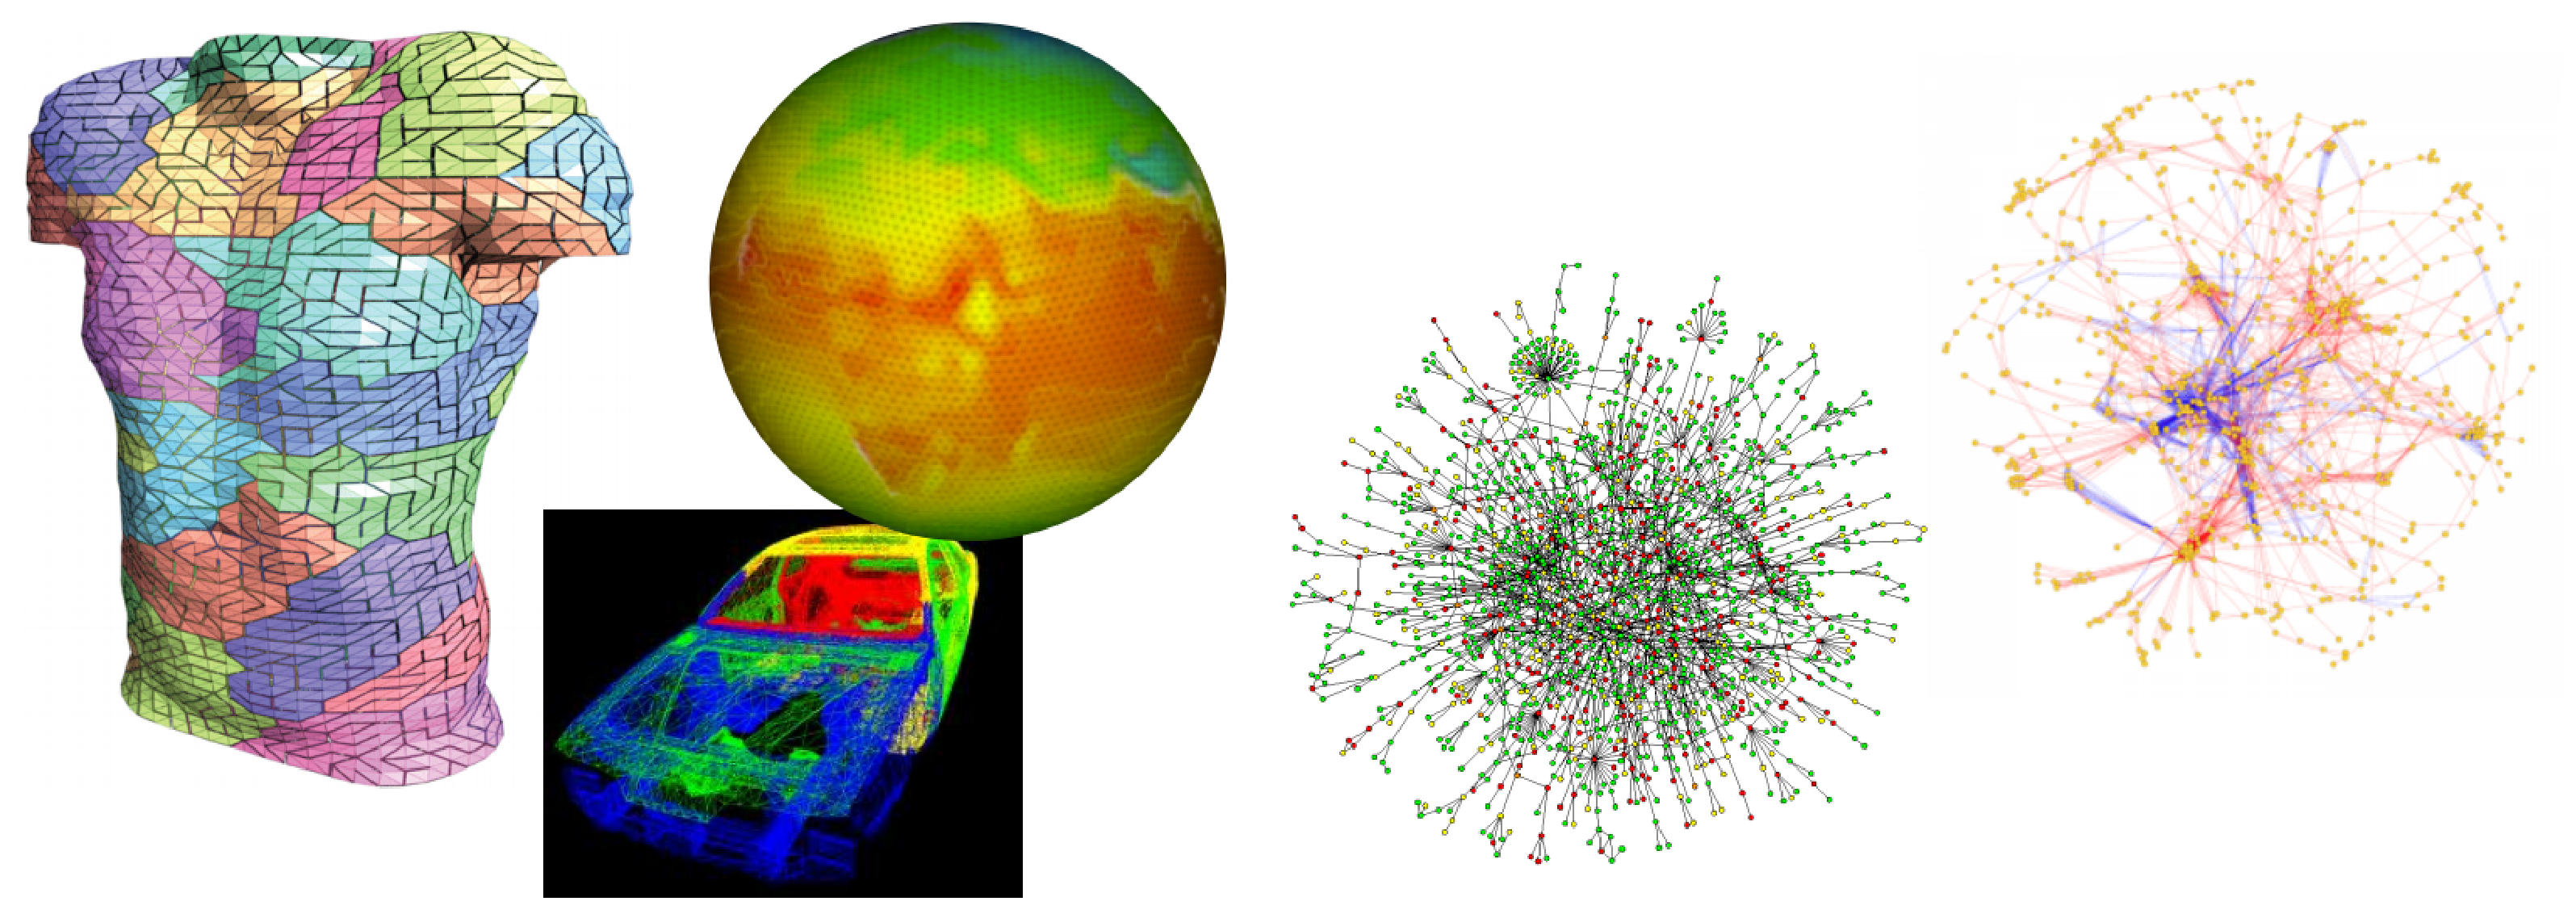
\includegraphics[width=0.9\textwidth]{graph/simulation.pdf}
  \end{figure}


  Modélisation de phénomènes physiques => opération sur des matrices.
\end{frame}

\begin{frame}
\frametitle{Ressources pour la simulation numérique}
  Un supercalculateur
  \uncover<2> {
    = plusieurs centaines (milliers) de nœuds !
  }
  \begin{figure}
    \only<1>{%
      
\includegraphics[width=\textwidth]{graph/supercomputer.pdf}%
    }%
    \only<2>{%
      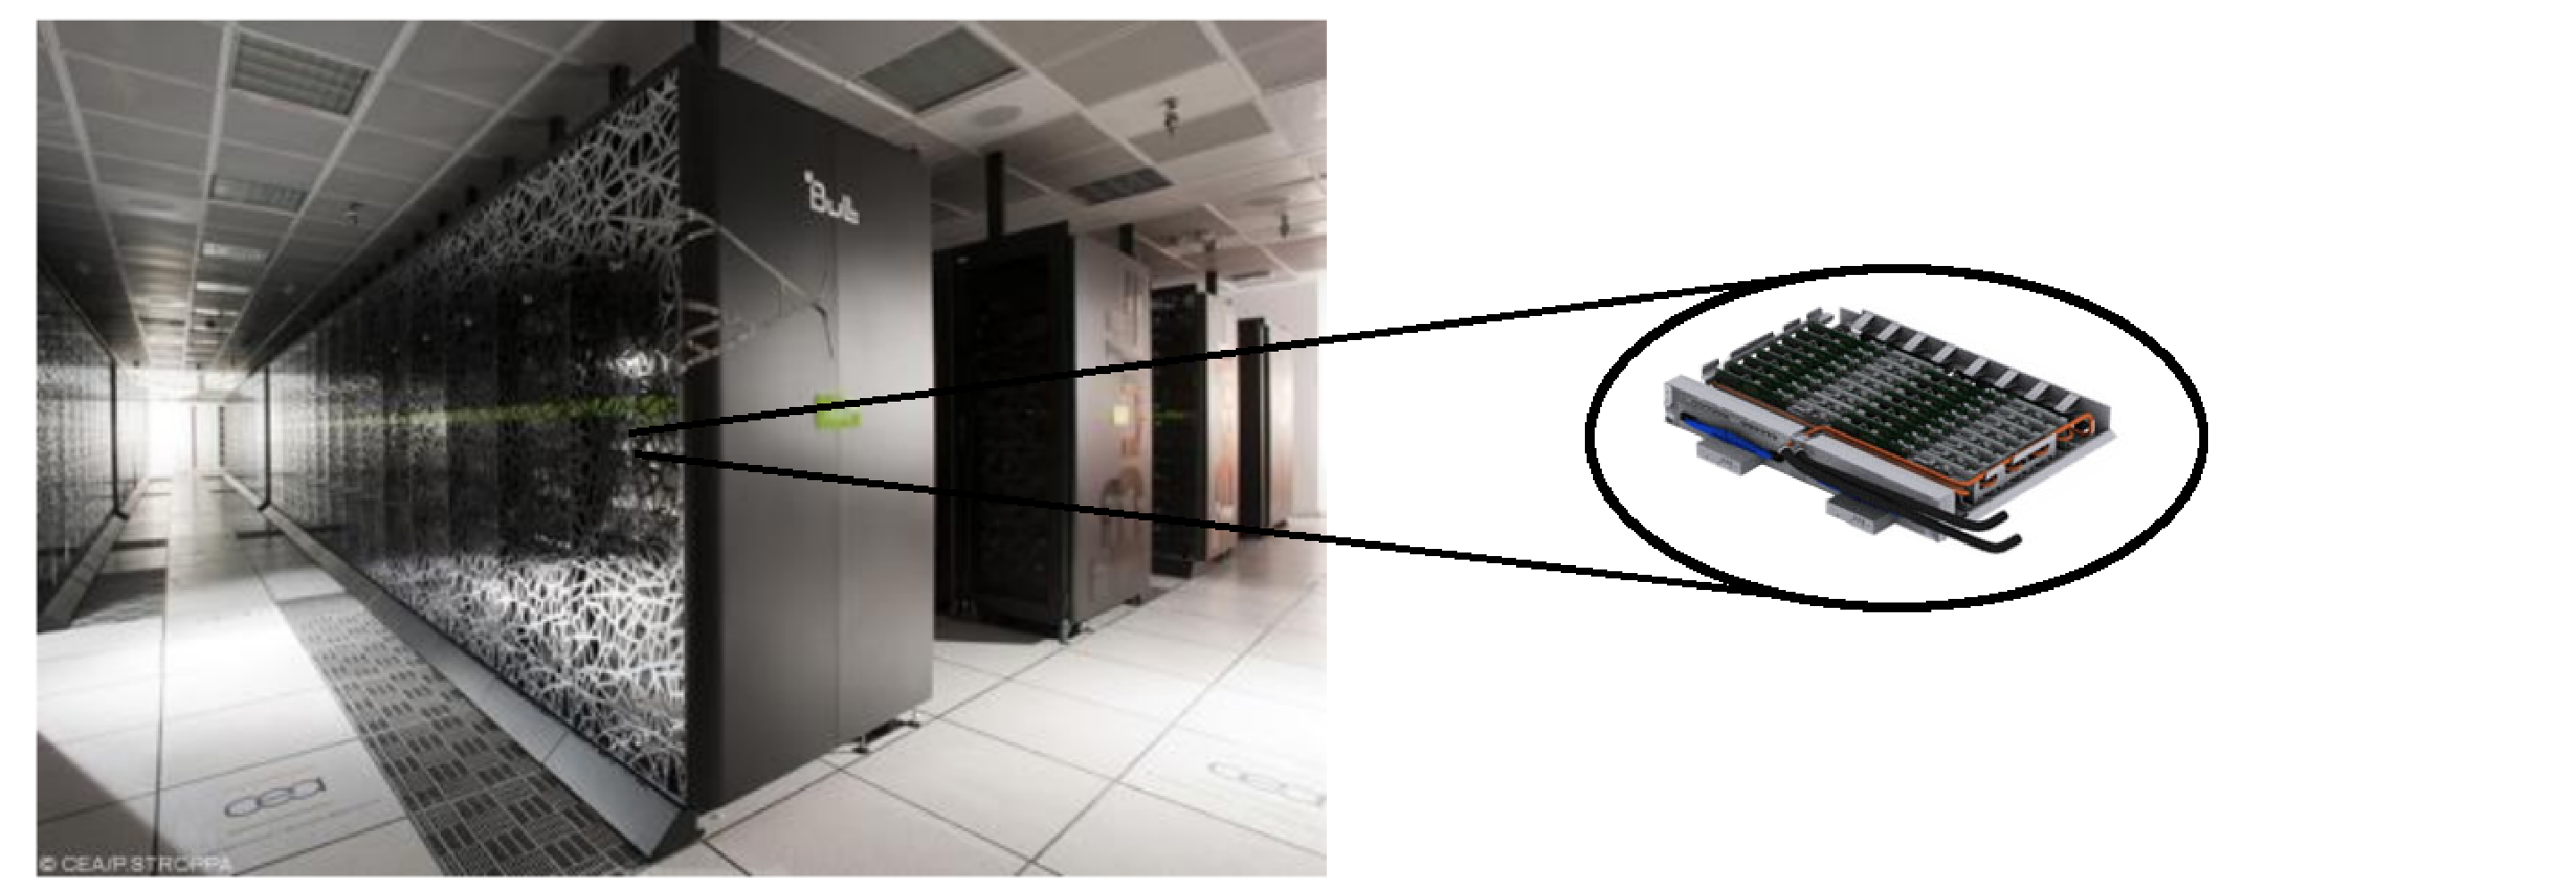
\includegraphics[width=\textwidth]{graph/supercomputer_with_node.pdf}%
    }%
  \end{figure}
\end{frame}

\begin{frame}
\frametitle{La barrière de péage}
  \begin{figure}
    %\only<1>{%
      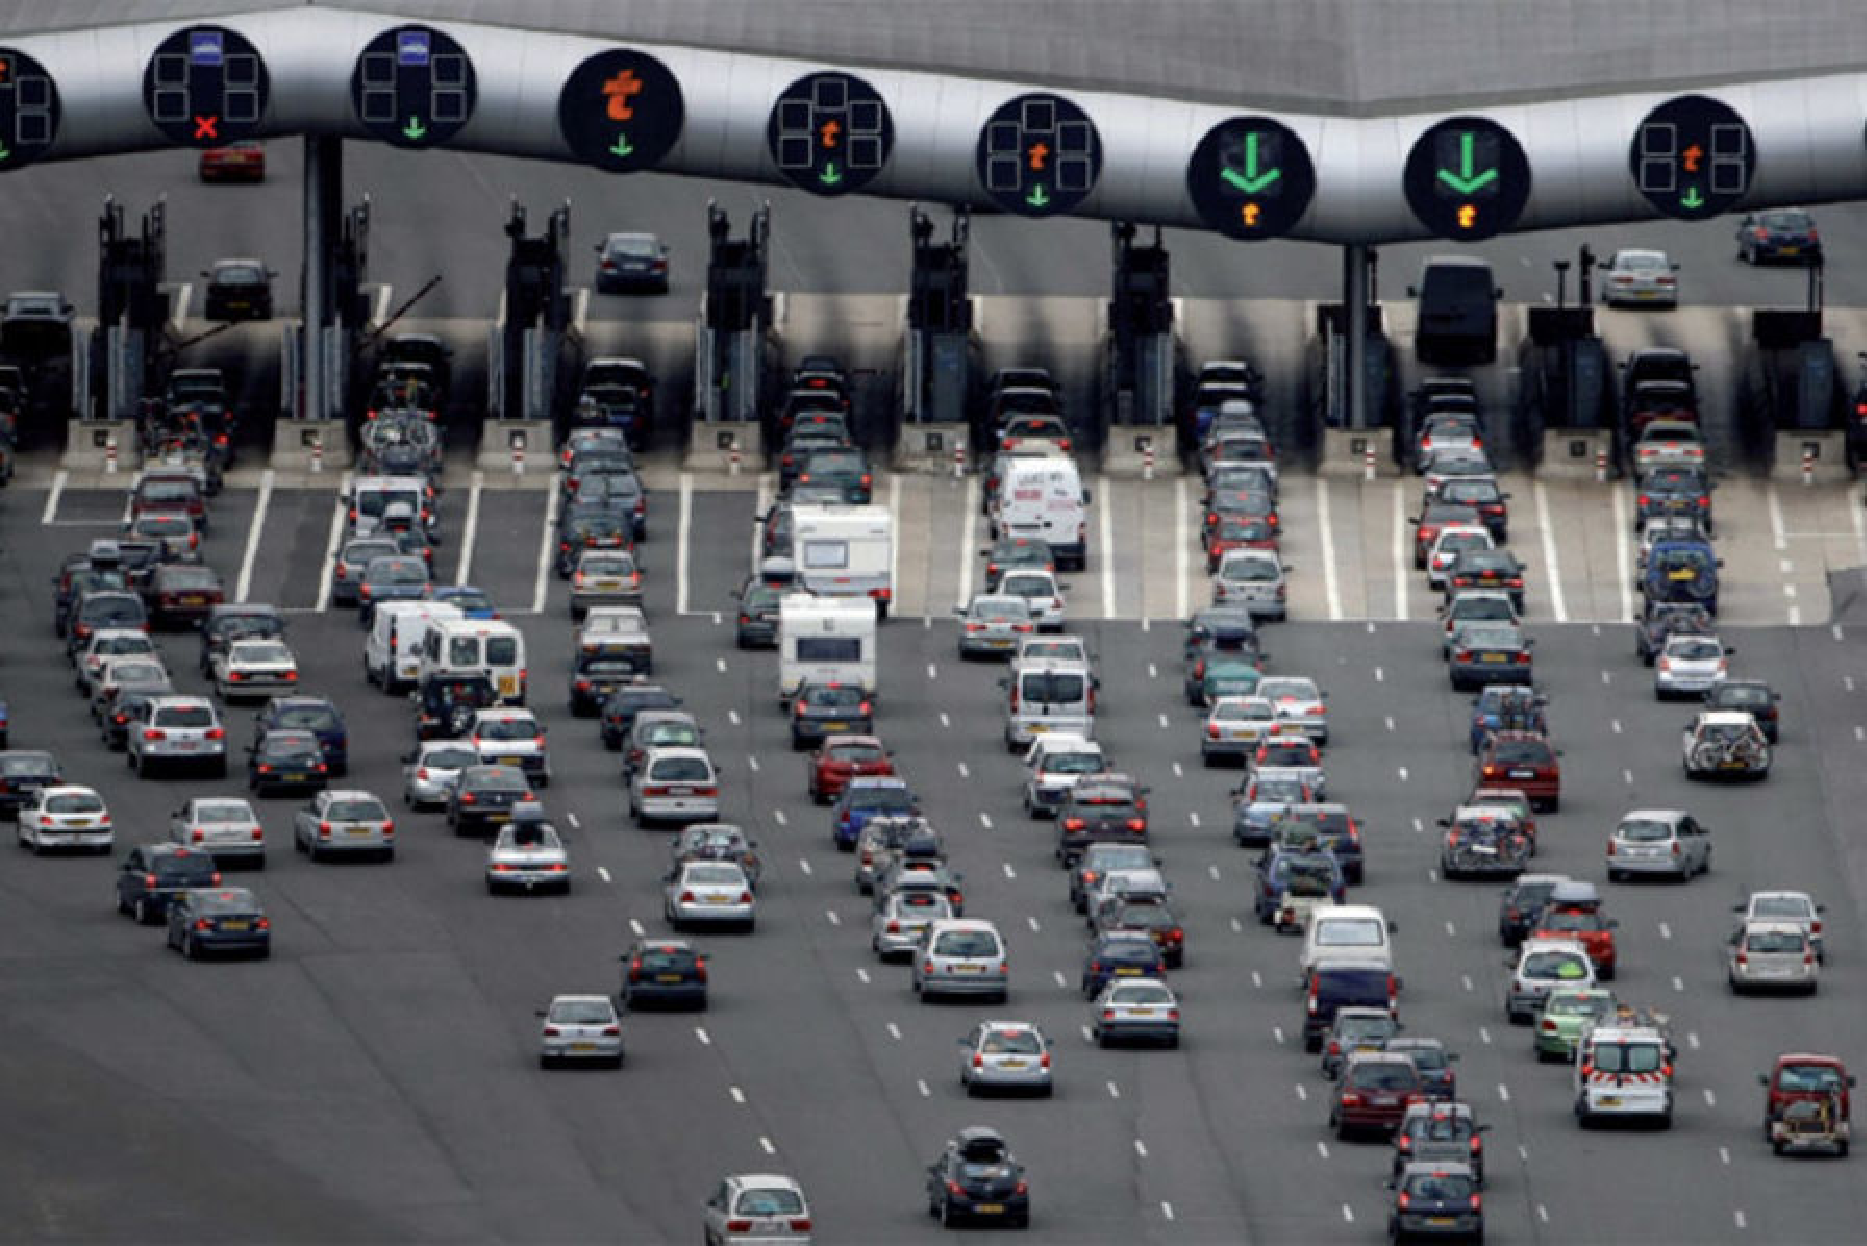
\includegraphics[width=\textwidth]{graph/peage.pdf}%
    %}%
    %\only<2>{%
      %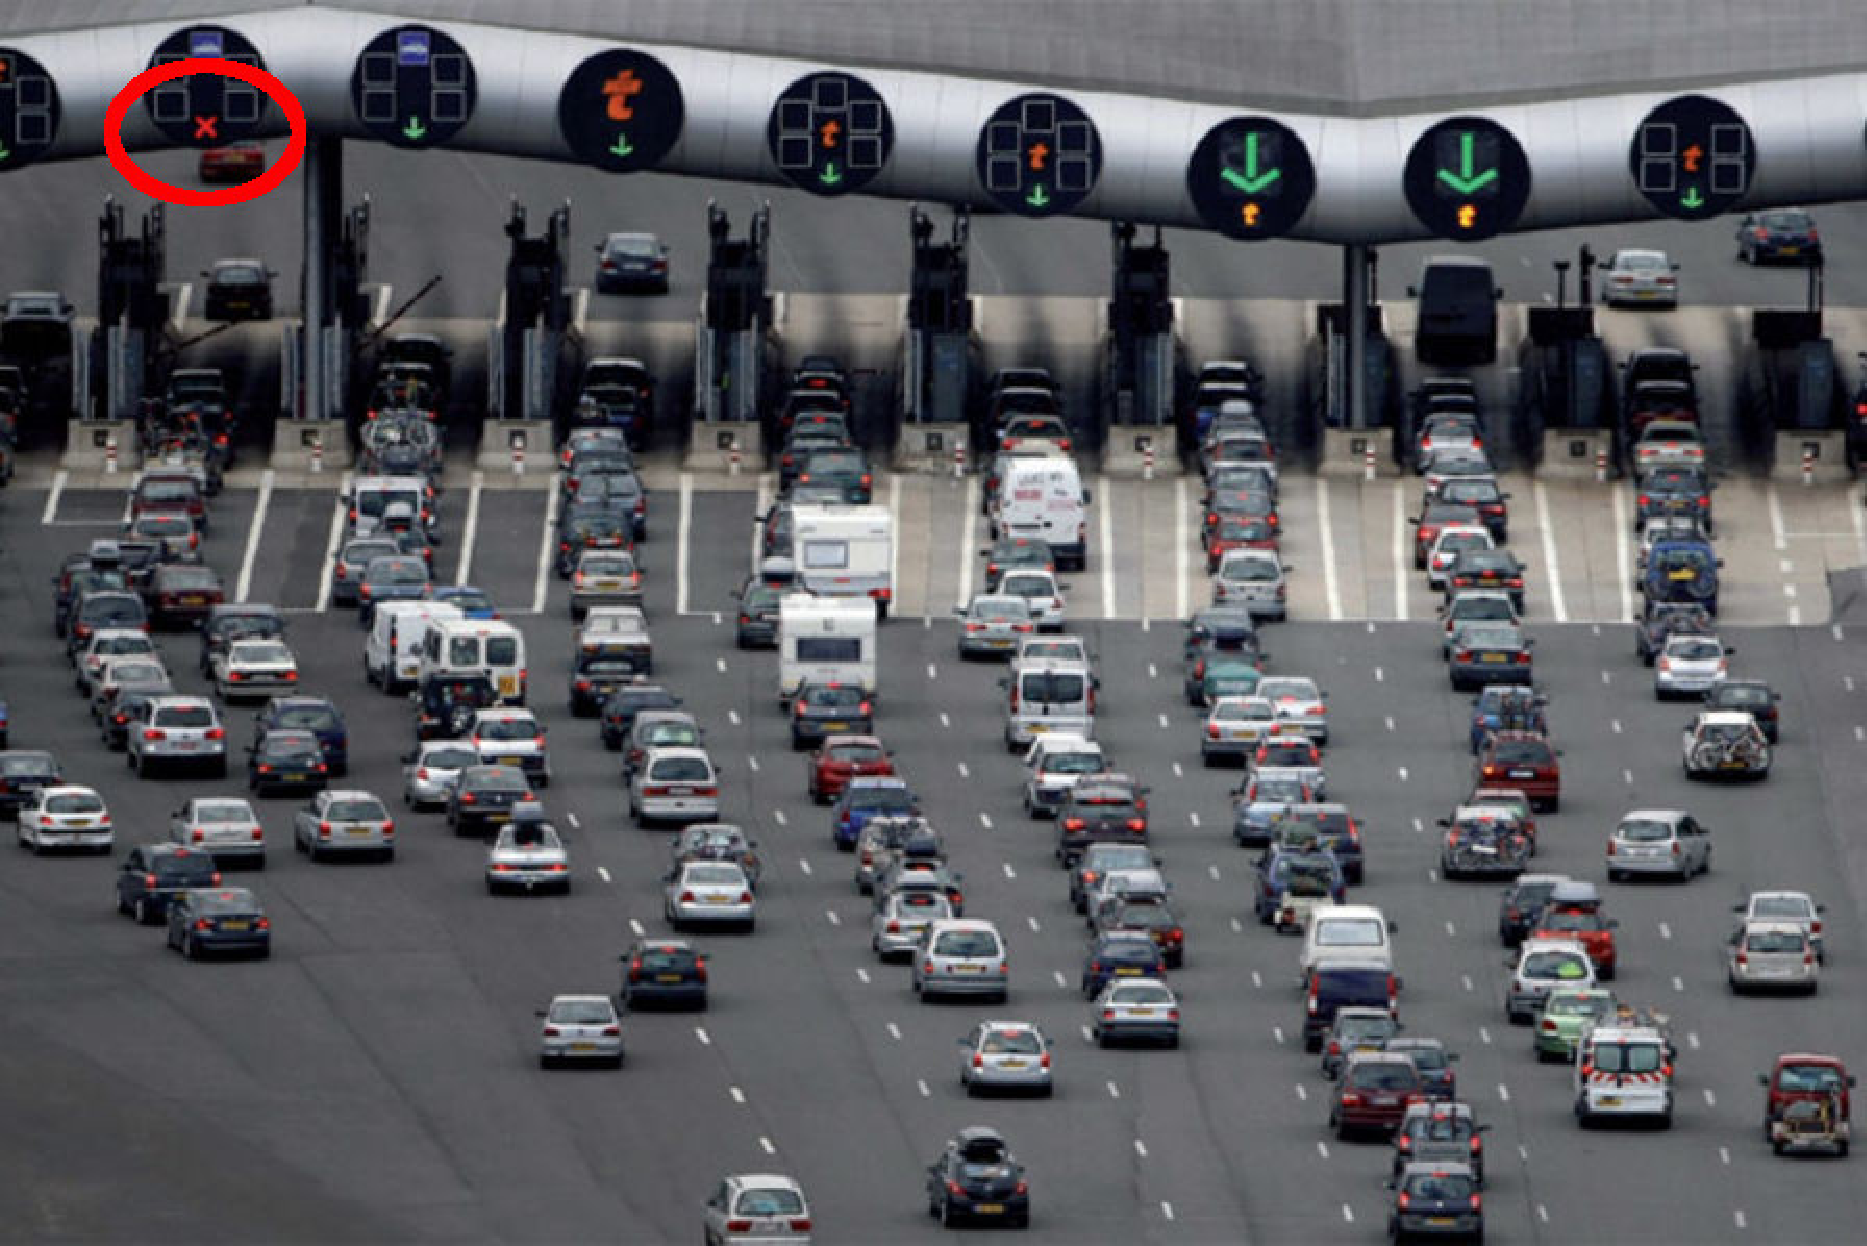
\includegraphics[width=\textwidth]{graph/peage-x.pdf}%
    %}%
    %\only<3>{%
      %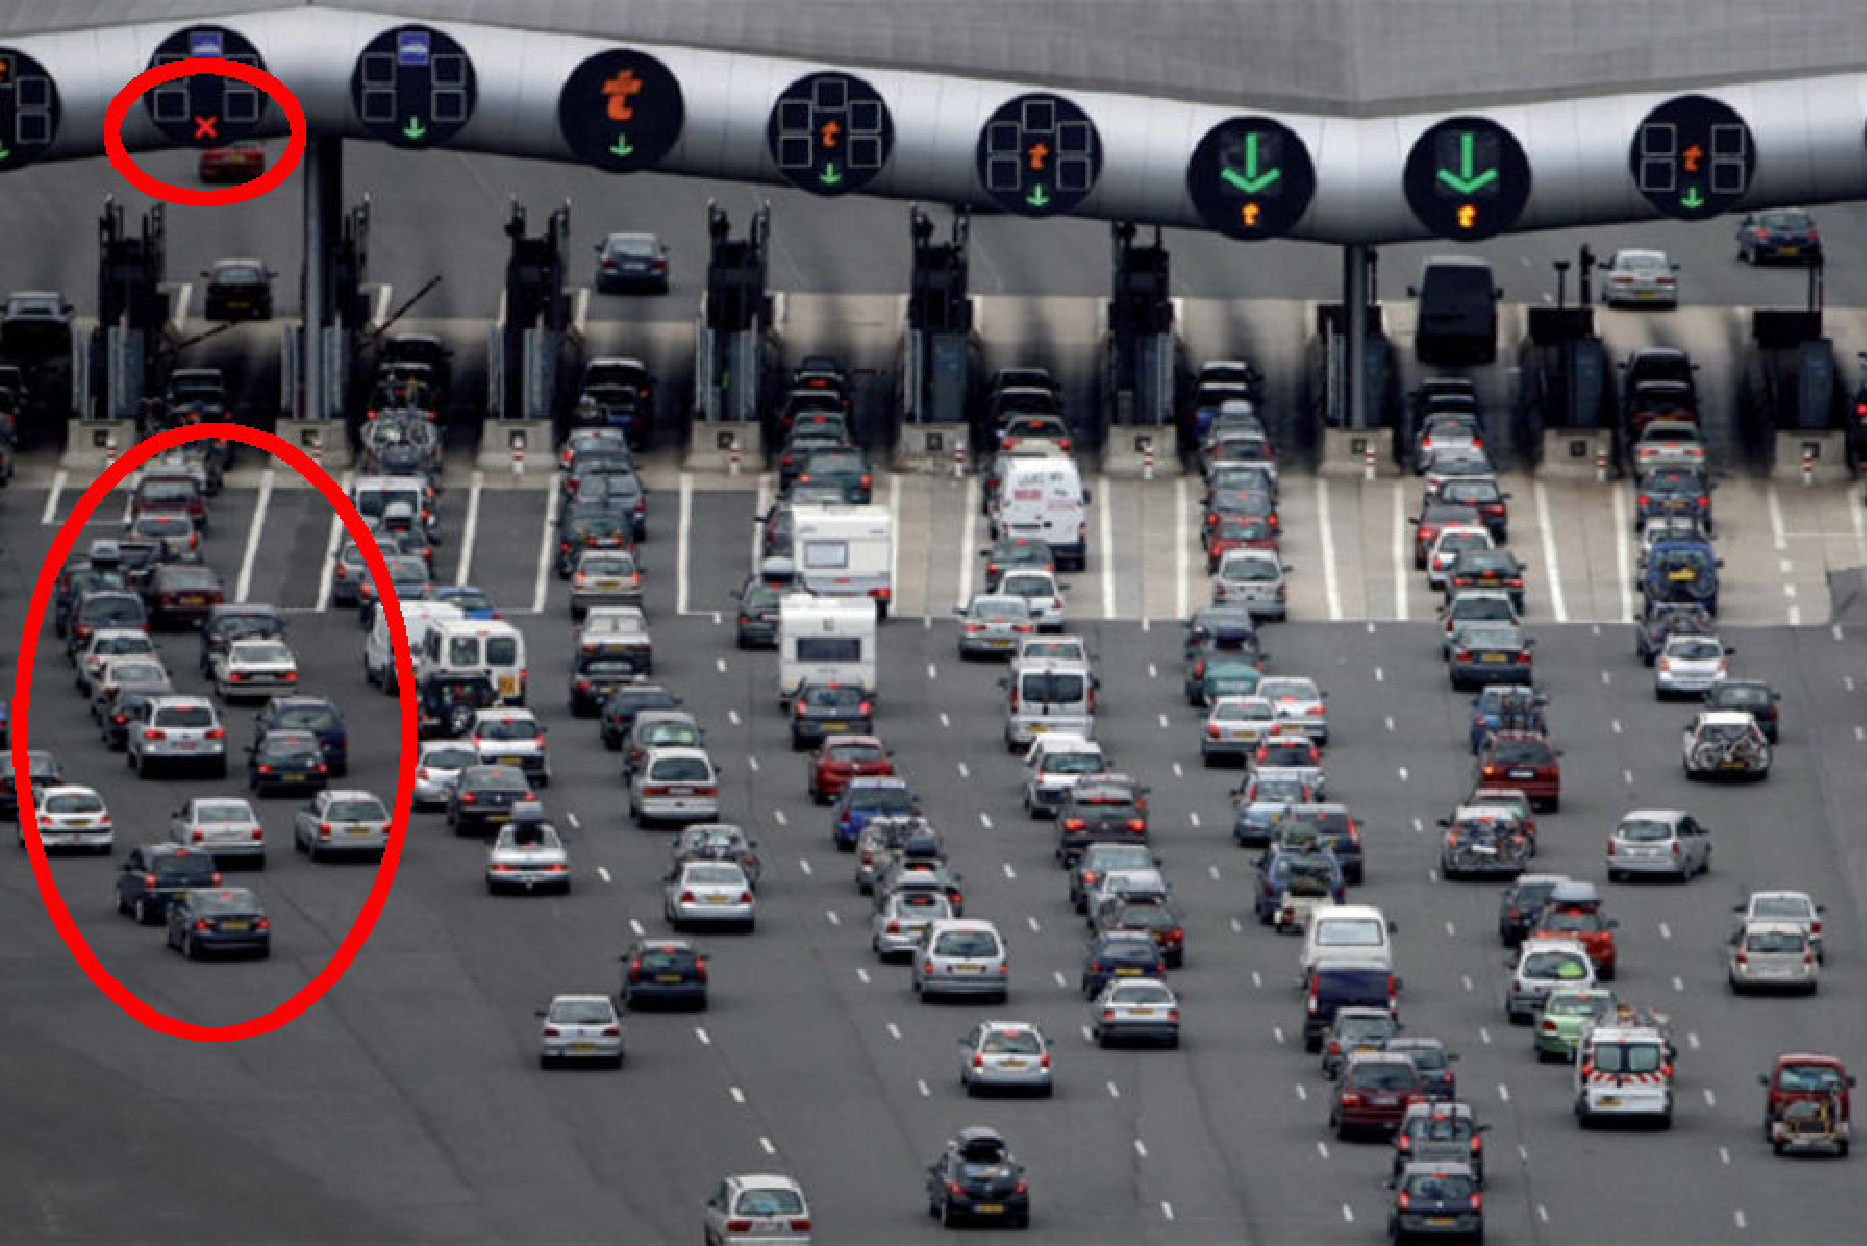
\includegraphics[width=\textwidth]{graph/peage-wtf.pdf}%
    %}%
  \end{figure}
\end{frame}

\begin{frame}
  \frametitle{Analogie avec l'ordinateur}
  \begin{figure}
    \only<1>{%
      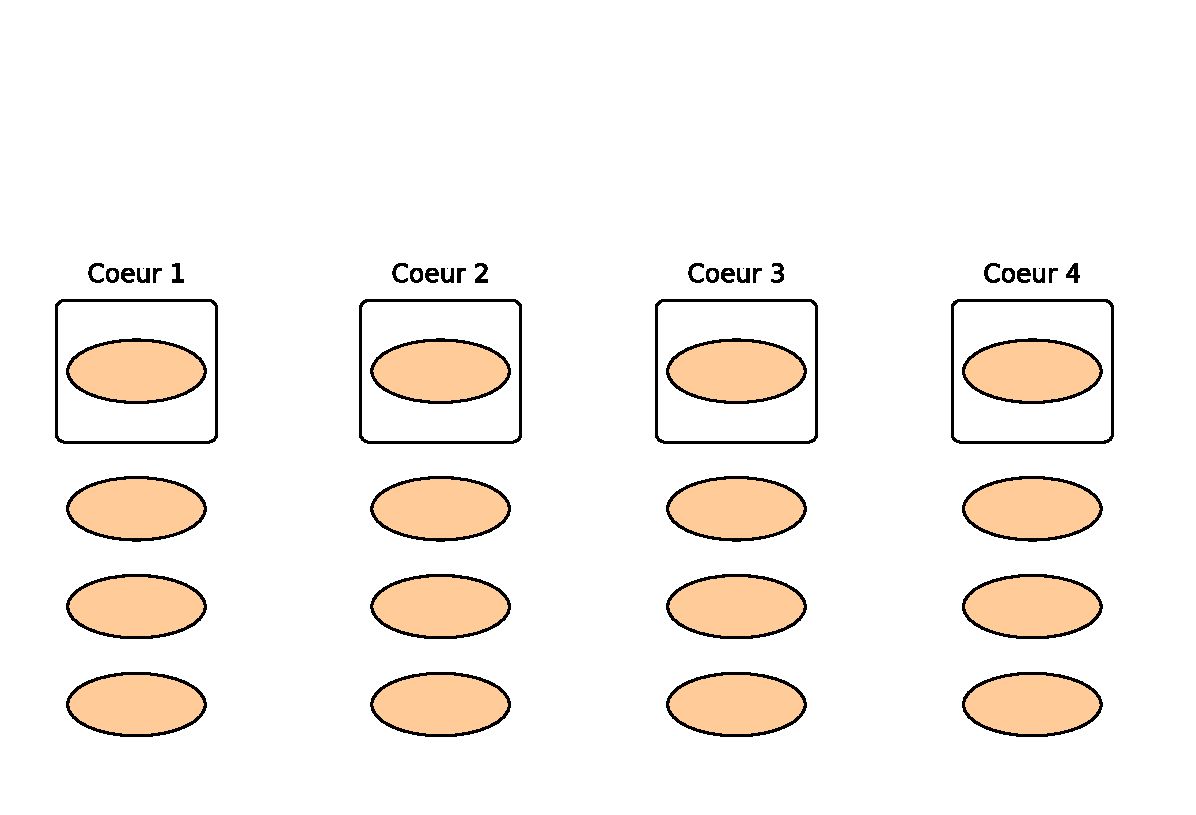
\includegraphics[width=0.8\textwidth]{graph/anim-peag/peage-analogie.pdf}%
    }%
    \only<2>{%
      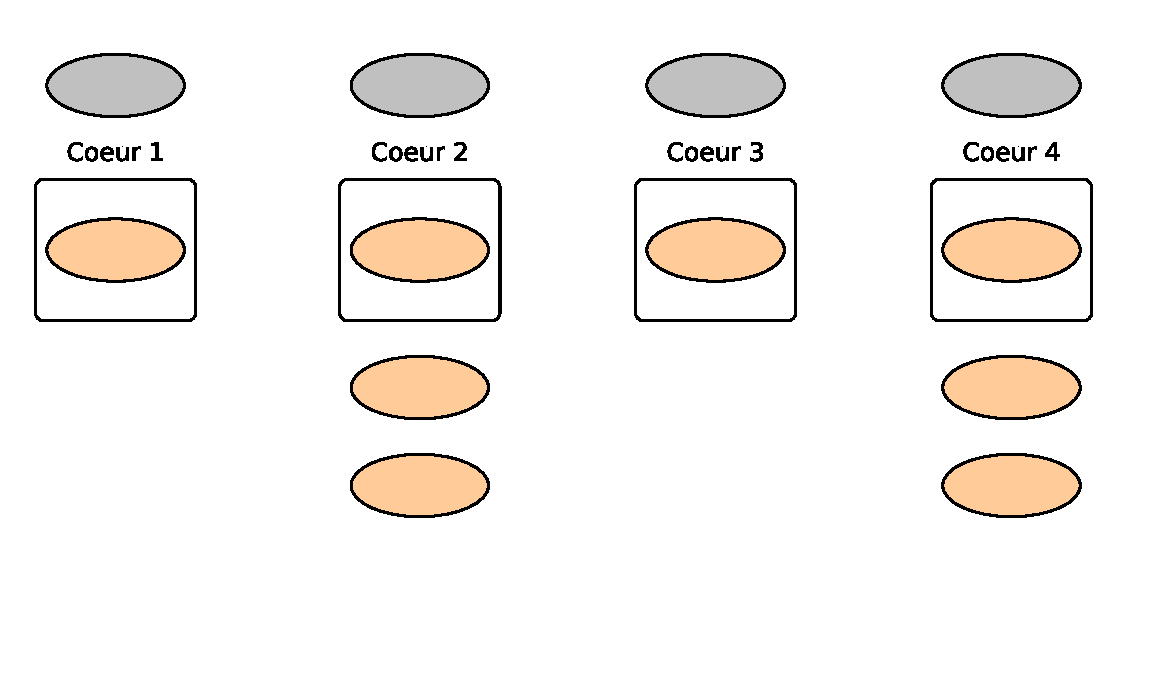
\includegraphics[width=0.8\textwidth]{graph/anim-peag/peage-analogie1.pdf}%
    }%
    \only<3>{%
      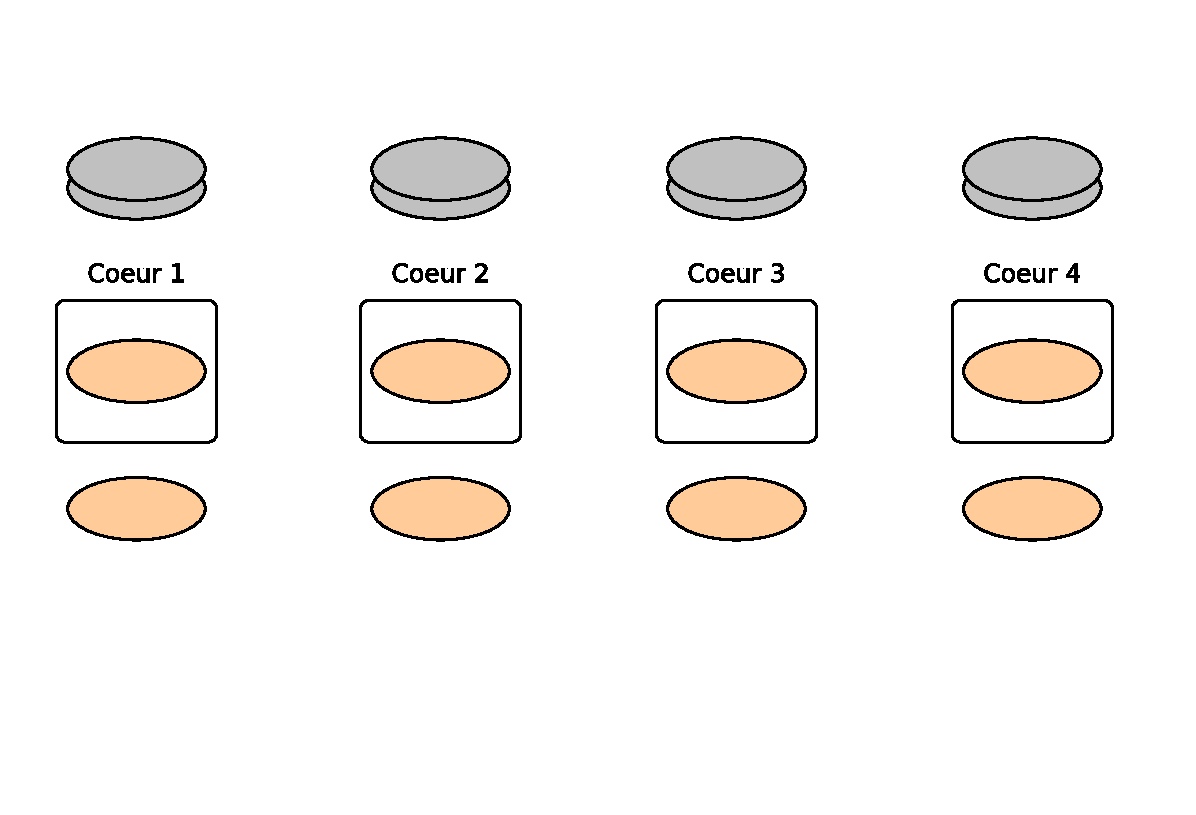
\includegraphics[width=0.8\textwidth]{graph/anim-peag/peage-analogie2.pdf}%
    }%
    \only<4>{%
      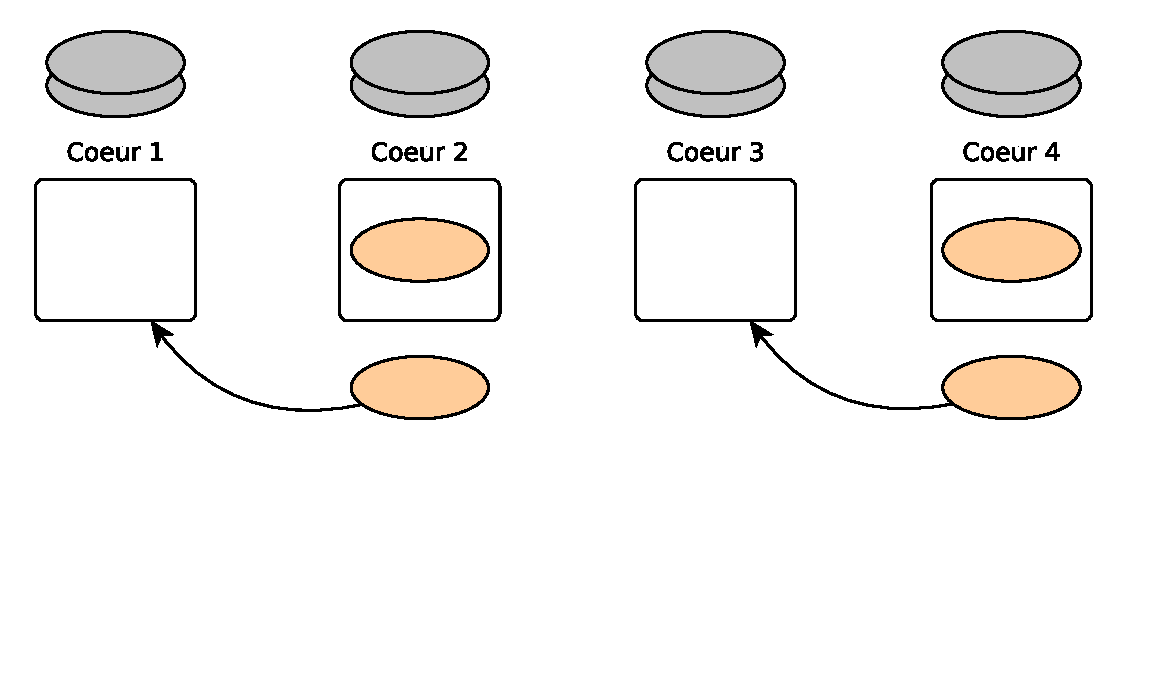
\includegraphics[width=0.8\textwidth]{graph/anim-peag/peage-analogie3.pdf}%
    }%
    \only<5>{%
      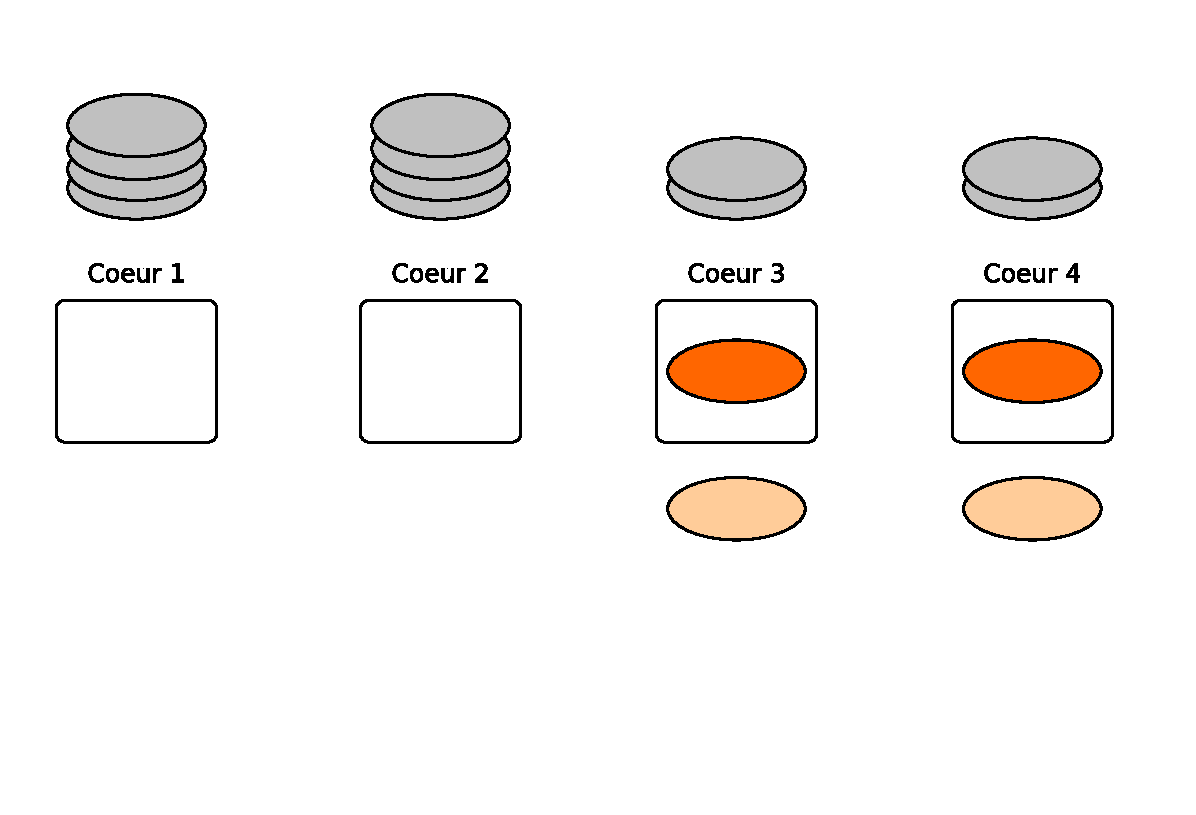
\includegraphics[width=0.8\textwidth]{graph/anim-peag/peage-analogie4.pdf}%
    }%
    \only<6>{%
      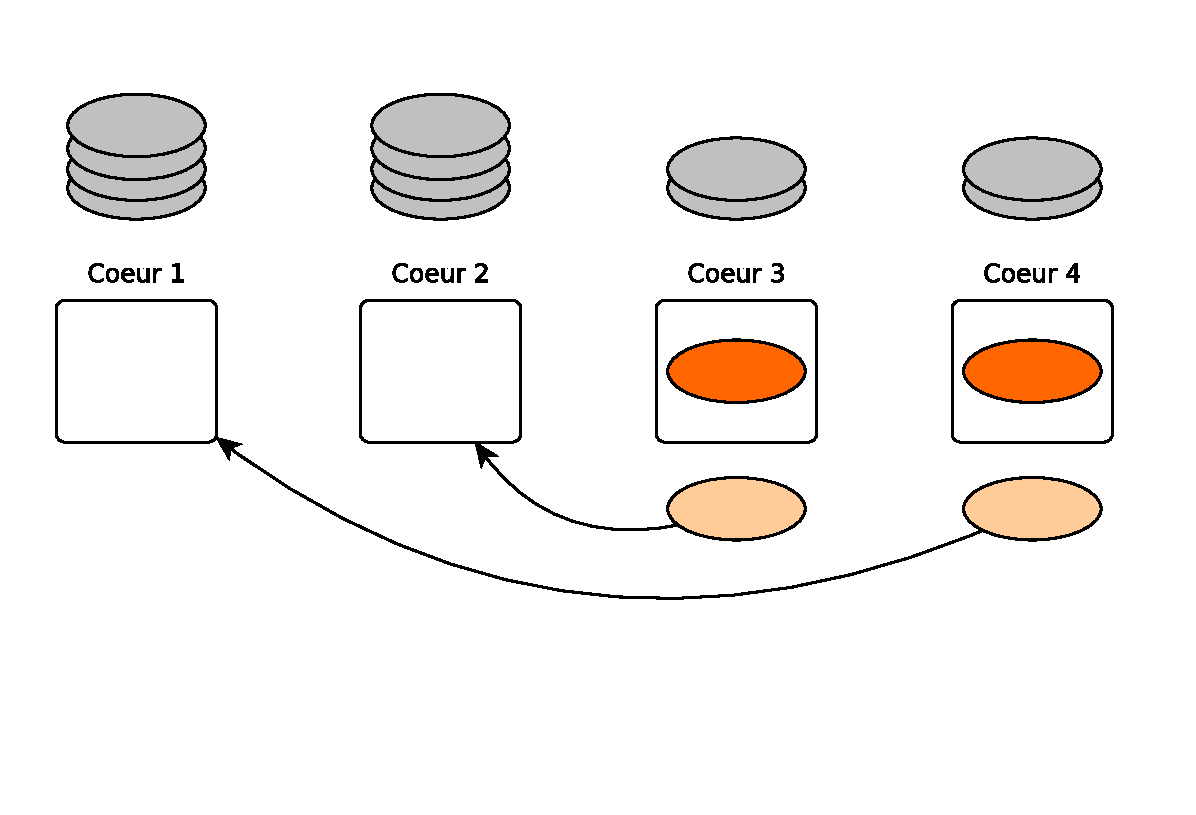
\includegraphics[width=0.8\textwidth]{graph/anim-peag/peage-analogie5.pdf}%
    }%
  \end{figure}
  \begin{figure}
    \centering
    
\includegraphics[width=0.7\textwidth]{graph/anim-peag/peage-analogie-legend.pdf}%
  \end{figure}
\end{frame}

\begin{frame}
\frametitle{Une application omniprésente : Cholesky}

Factorisation d'une matrice symétrique positive définie $A$ :
$$ A = L*L^T$$

\begin{itemize}
\item Très utilisée pour la résolution de systèmes d'équations.

\item Plusieurs versions

  \begin{itemize}
    \item Linpack
    \item Lapack (bloc ligne/colonne)
    \item "à la Plasma" -> parallèle par blocs
  \end{itemize}
\end{itemize}

\end{frame}

\begin{frame}[fragile]
\frametitle{Une application omniprésente : Cholesky}

Description des opérations et de leur ordre :

\noindent{%
\begin{minipage}[t]{0.38\linewidth}
  \begin{block}{Noyaux:}
    \begin{itemize}
      \item \potrf Cholesky
      \item \trsm Résolution d'un système triangulaire
      \item \gemm Multiplication de matrices
      \item \syrk Multiplication de matrices symétriques
    \end{itemize}
  \end{block}
\end{minipage}}%
\hfill%
\begin{minipage}[t]{0.54\linewidth}
  \begin{figure}
    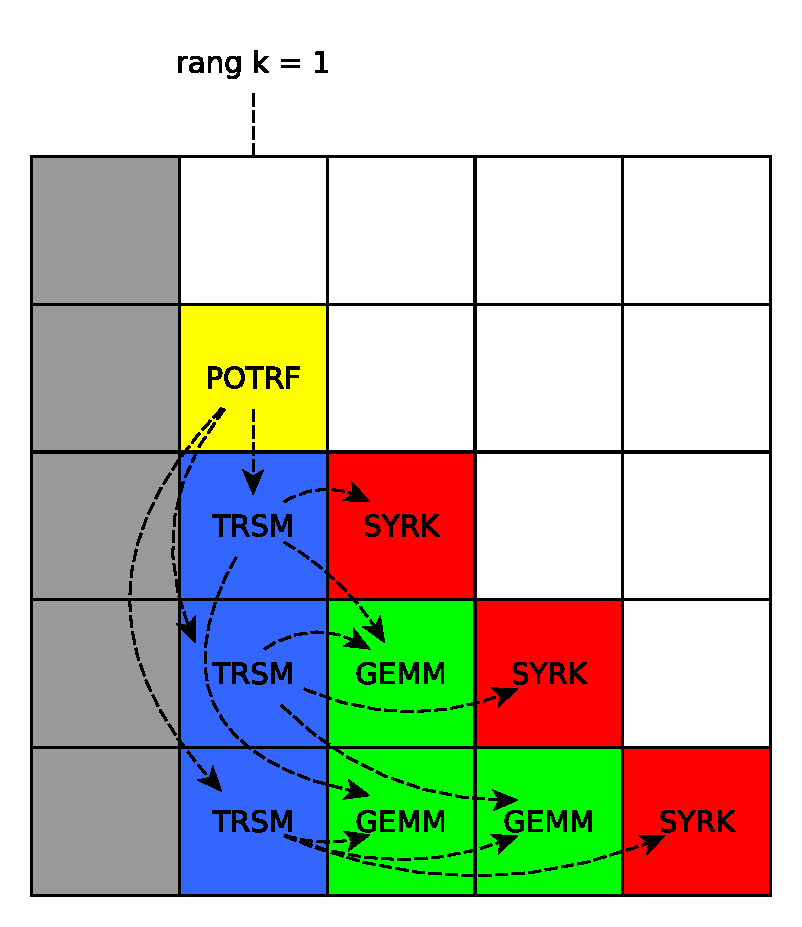
\includegraphics[width=\textwidth]{graph/cholesky-rank-update.pdf}
  \end{figure}
\end{minipage}


\end{frame}

\begin{frame}
\frametitle{Une application omniprésente : Cholesky}

Exprimée dans un langage par flot de données, et représentation de l'application sous forme de graphe :
\begin{figure}
  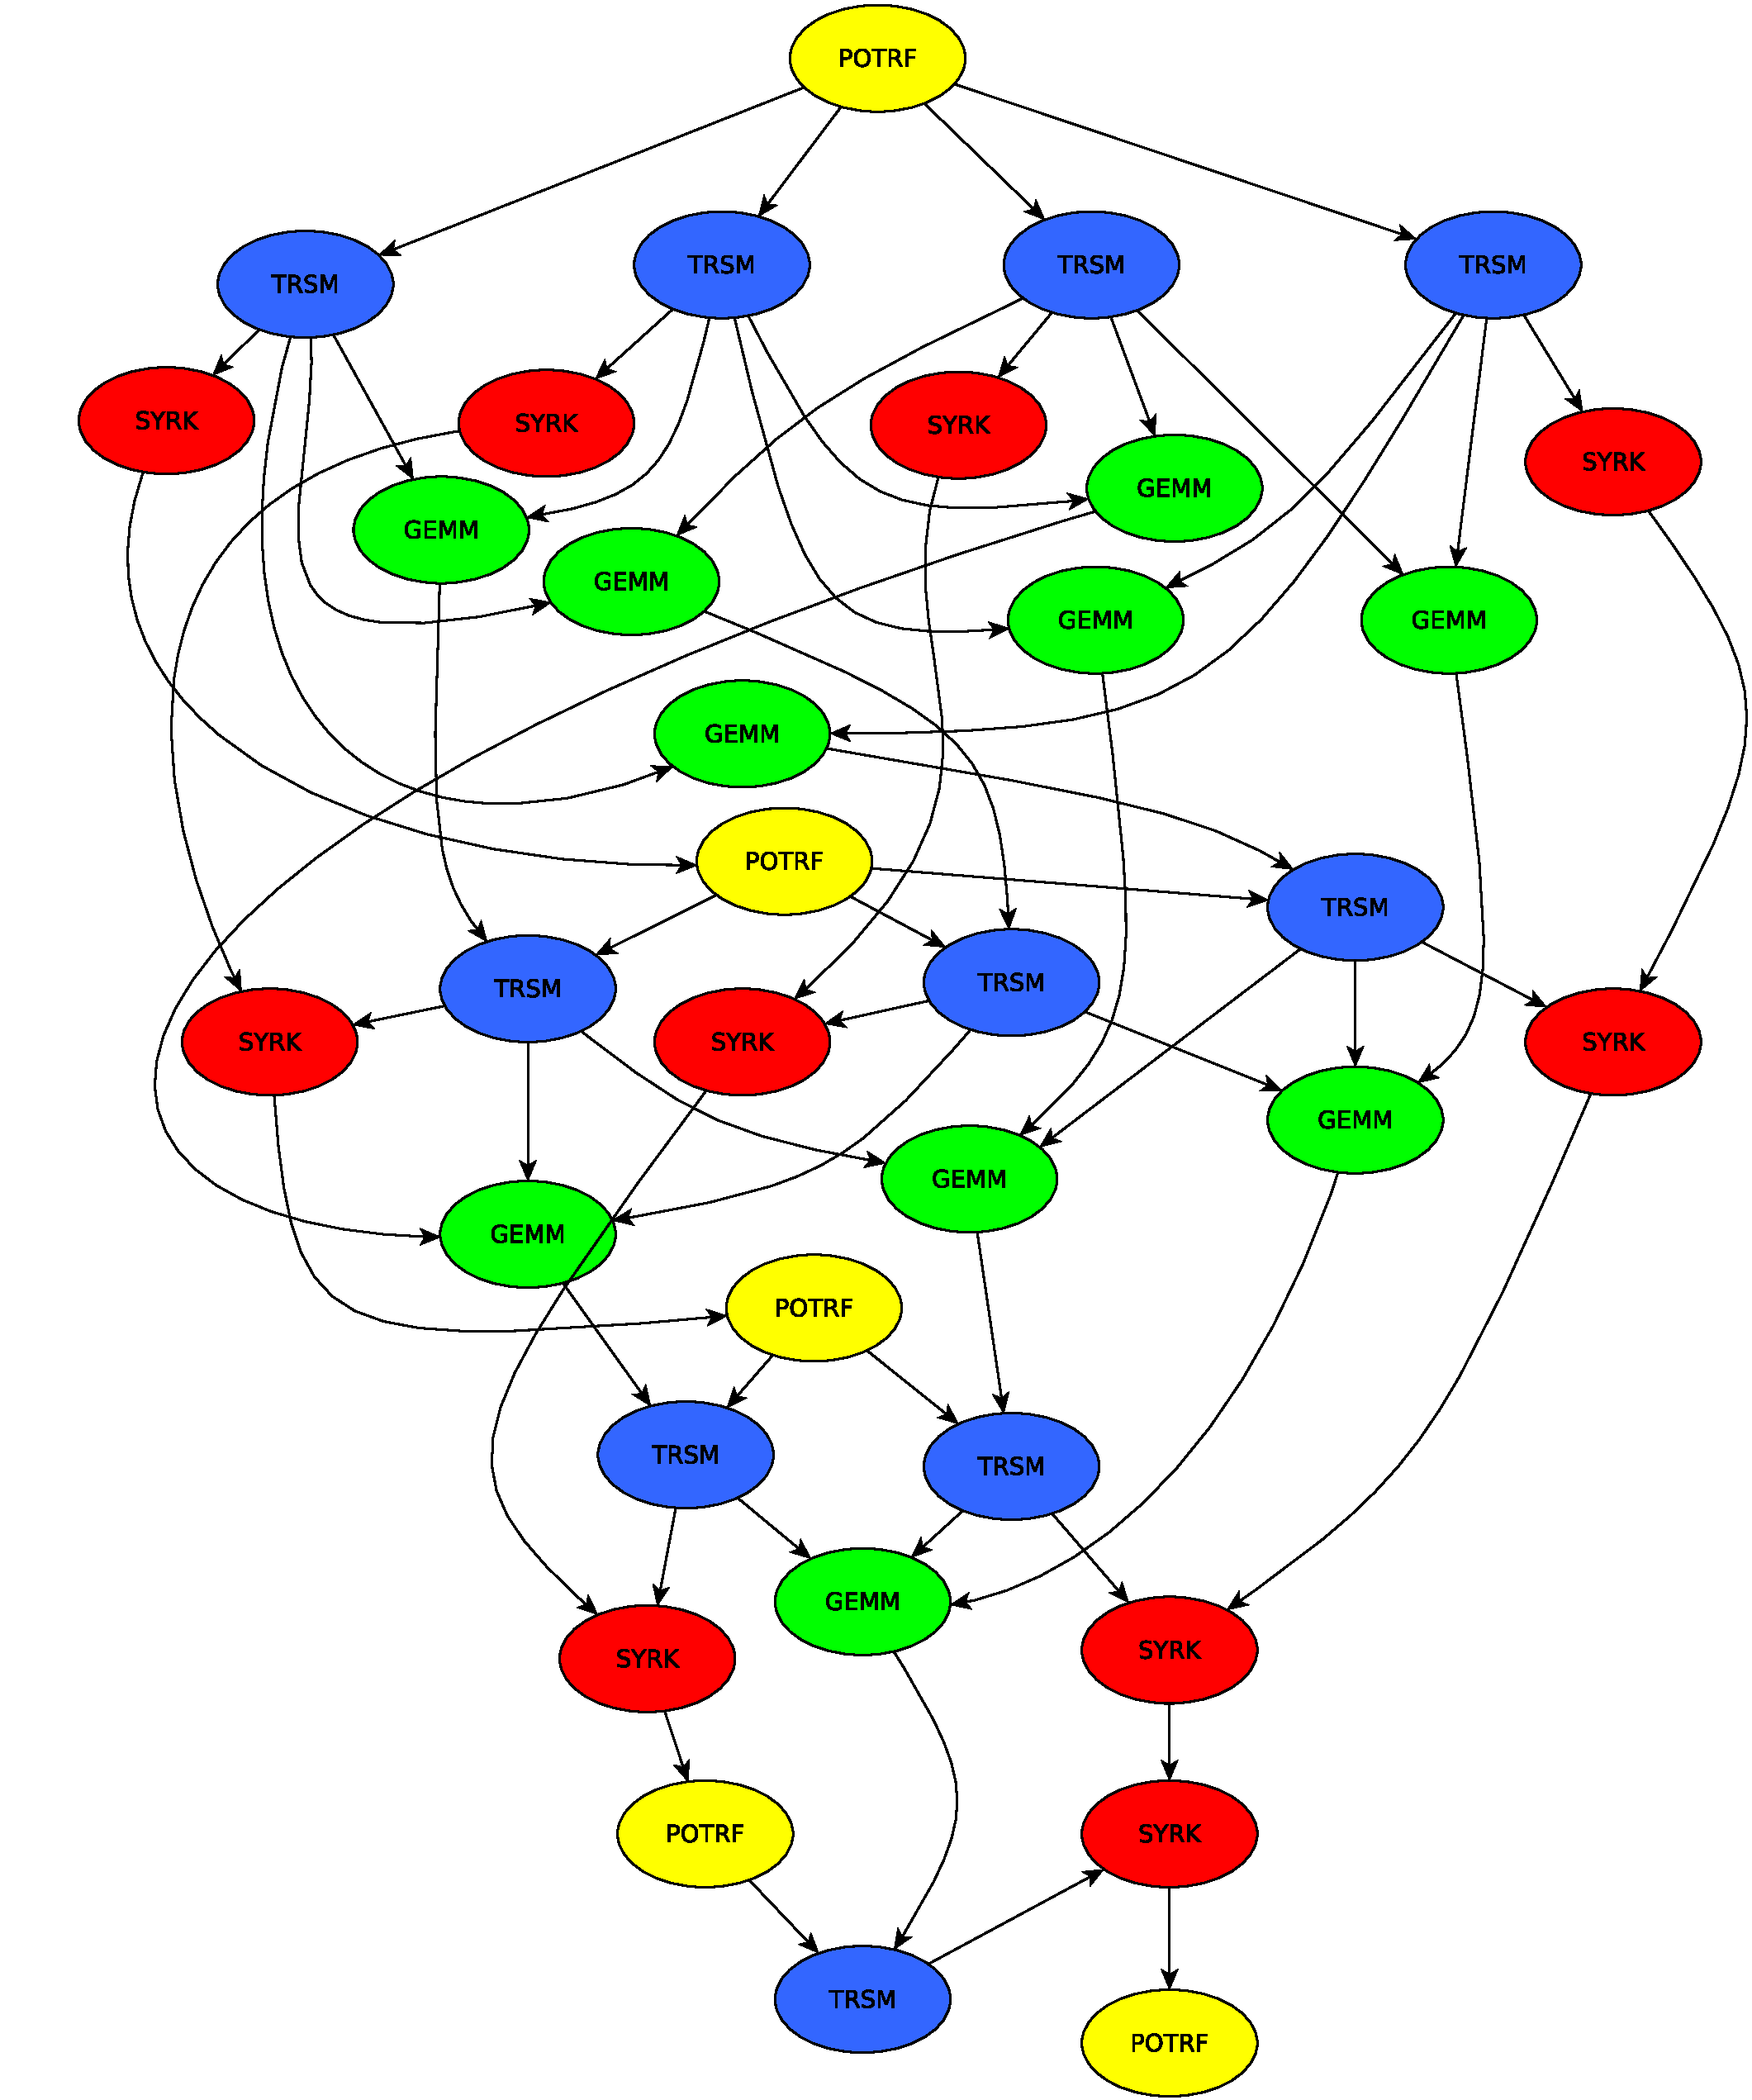
\includegraphics[width=0.4\textwidth]{graph/cholesky-dag-5.pdf}
\end{figure}


\end{frame}

\begin{frame}[fragile]
\frametitle{Expression dans un modèle de programmation : OpenMP}

\begin{minipage}[t]{0.52\linewidth}
  \vspace{0.3cm}
  \begin{onlyenv}<1>
  \begin{lstlisting}[language=c]
#define N_BLOCS 3
for (int k = 0; k < N_BLOCS; k++) {
  #pragma omp task depend(inout:A(k,k))
  POTRF(A(k, k));

  //...
}
  \end{lstlisting}
\end{onlyenv}
  \begin{onlyenv}<2>
  \begin{lstlisting}[style=transparency]
@#define N_BLOCS 3
for (int k = 0; k < N_BLOCS; k++) {
  #pragma omp task depend(inout:A(k,k))
  POTRF(A(k, k));@

  for (int m = k+1; m < N_BLOCS; m++) {
    #pragma omp task depend(in:A(k,k))
                     depend(inout:A(m,k))
    TRSM(A(k, k), A(m, k));
  }

  @//...
}@
  \end{lstlisting}
\end{onlyenv}
  \begin{onlyenv}<3>
  \begin{lstlisting}[style=transparency]
@#define N_BLOCS 3
for (int k = 0; k < N_BLOCS; k++) {
  #pragma omp task depend(inout:A(k,k))
  POTRF(A(k, k));

  for (int m = k+1; m < N_BLOCS; m++) {
    #pragma omp task depend(in:A(k,k))
                     depend(inout:A(m,k))
    TRSM(A(k, k), A(m, k));
  }@

  for (int m = k+1; m < N_BLOCS; m++) {
    #pragma omp task depend(in:A(m,k))
                     depend(inout:A(k,k))
    SYRK(A(m, k), A(k, k));

    @//...
  }
}@
  \end{lstlisting}
\end{onlyenv}
  \begin{onlyenv}<4>
  \begin{lstlisting}[style=transparency]
@#define N_BLOCS 3
for (int k = 0; k < N_BLOCS; k++) {
  #pragma omp task depend(inout:A(k,k))
  POTRF(A(k, k));

  for (int m = k+1; m < N_BLOCS; m++) {
    #pragma omp task depend(in:A(k,k))
                     depend(inout:A(m,k))
    TRSM(A(k, k), A(m, k));
  }

  for (int m = k+1; m < N_BLOCS; m++) {
    #pragma omp task depend(in:A(m,k))
                     depend(inout:A(k,k))
    SYRK(A(m, k), A(k, k));@

    for (int n = k+1; n < m; n++) {
      #pragma omp task depend(in:A(m,k), A(n,k))
                       depend(inout:A(m,n))
      GEMM(A(n, k), A(m, k), A(m, n));
    }@
  }
}@
  \end{lstlisting}
\end{onlyenv}
  \begin{onlyenv}<5>
  \begin{lstlisting}[style=transparency]
@#define N_BLOCS 3
for (int k = 0; k < N_BLOCS; k++) {@
  #pragma omp task depend(inout:A(k,k))
  POTRF(A(k, k));

  @for (int m = k+1; m < N_BLOCS; m++) {
    #pragma omp task depend(in:A(k,k))
                     depend(inout:A(m,k))
    TRSM(A(k, k), A(m, k));
  }

  for (int m = k+1; m < N_BLOCS; m++) {
    #pragma omp task depend(in:A(m,k))
                     depend(inout:A(k,k))
    SYRK(A(m, k), A(k, k));

    for (int n = k+1; n < m; n++) {
      #pragma omp task depend(in:A(m,k), A(n,k))
                       depend(inout:A(m,n))
      GEMM(A(n, k), A(m, k), A(m, n));
    }
  }
}@
  \end{lstlisting}
\end{onlyenv}
  \begin{onlyenv}<6>
  \begin{lstlisting}[style=transparency]
@#define N_BLOCS 3
for (int k = 0; k < N_BLOCS; k++) {
  #pragma omp task depend(inout:A(k,k))
  POTRF(A(k, k));@

  for (int m = k+1; m < N_BLOCS; m++) {
    #pragma omp task depend(in:A(k,k))
                     depend(inout:A(m,k))
    TRSM(A(k, k), A(m, k));
  }@

  for (int m = k+1; m < N_BLOCS; m++) {
    #pragma omp task depend(in:A(m,k))
                     depend(inout:A(k,k))
    SYRK(A(m, k), A(k, k));

    for (int n = k+1; n < m; n++) {
      #pragma omp task depend(in:A(m,k), A(n,k))
                       depend(inout:A(m,n))
      GEMM(A(n, k), A(m, k), A(m, n));
    }
  }
}@
  \end{lstlisting}
\end{onlyenv}
  \begin{onlyenv}<7>
  \begin{lstlisting}[style=transparency]
@#define N_BLOCS 3
for (int k = 0; k < N_BLOCS; k++) {
  #pragma omp task depend(inout:A(k,k))
  POTRF(A(k, k));

  for (int m = k+1; m < N_BLOCS; m++) {
    #pragma omp task depend(in:A(k,k))
                     depend(inout:A(m,k))
    TRSM(A(k, k), A(m, k));
  }@

  for (int m = k+1; m < N_BLOCS; m++) {
    #pragma omp task depend(in:A(m,k))
                     depend(inout:A(k,k))
    SYRK(A(m, k), A(k, k));

    @for (int n = k+1; n < m; n++) {
      #pragma omp task depend(in:A(m,k), A(n,k))
                       depend(inout:A(m,n))
      GEMM(A(n, k), A(m, k), A(m, n));
    }
  }
}@
  \end{lstlisting}
\end{onlyenv}
  \begin{onlyenv}<8>
  \begin{lstlisting}[style=transparency]
@#define N_BLOCS 3
for (int k = 0; k < N_BLOCS; k++) {@
  #pragma omp task depend(inout:A(k,k))
  POTRF(A(k, k));@

  for (int m = k+1; m < N_BLOCS; m++) {
    #pragma omp task depend(in:A(k,k))
                     depend(inout:A(m,k))
    TRSM(A(k, k), A(m, k));
  }

  for (int m = k+1; m < N_BLOCS; m++) {
    #pragma omp task depend(in:A(m,k))
                     depend(inout:A(k,k))
    SYRK(A(m, k), A(k, k));

    for (int n = k+1; n < m; n++) {
      #pragma omp task depend(in:A(m,k), A(n,k))
                       depend(inout:A(m,n))
      GEMM(A(n, k), A(m, k), A(m, n));
    }
  }
}@
  \end{lstlisting}
\end{onlyenv}
\end{minipage}
\begin{minipage}[t]{0.46\linewidth}
  \vspace{-0.3cm}
\begin{figure}
  \only<1>{%
    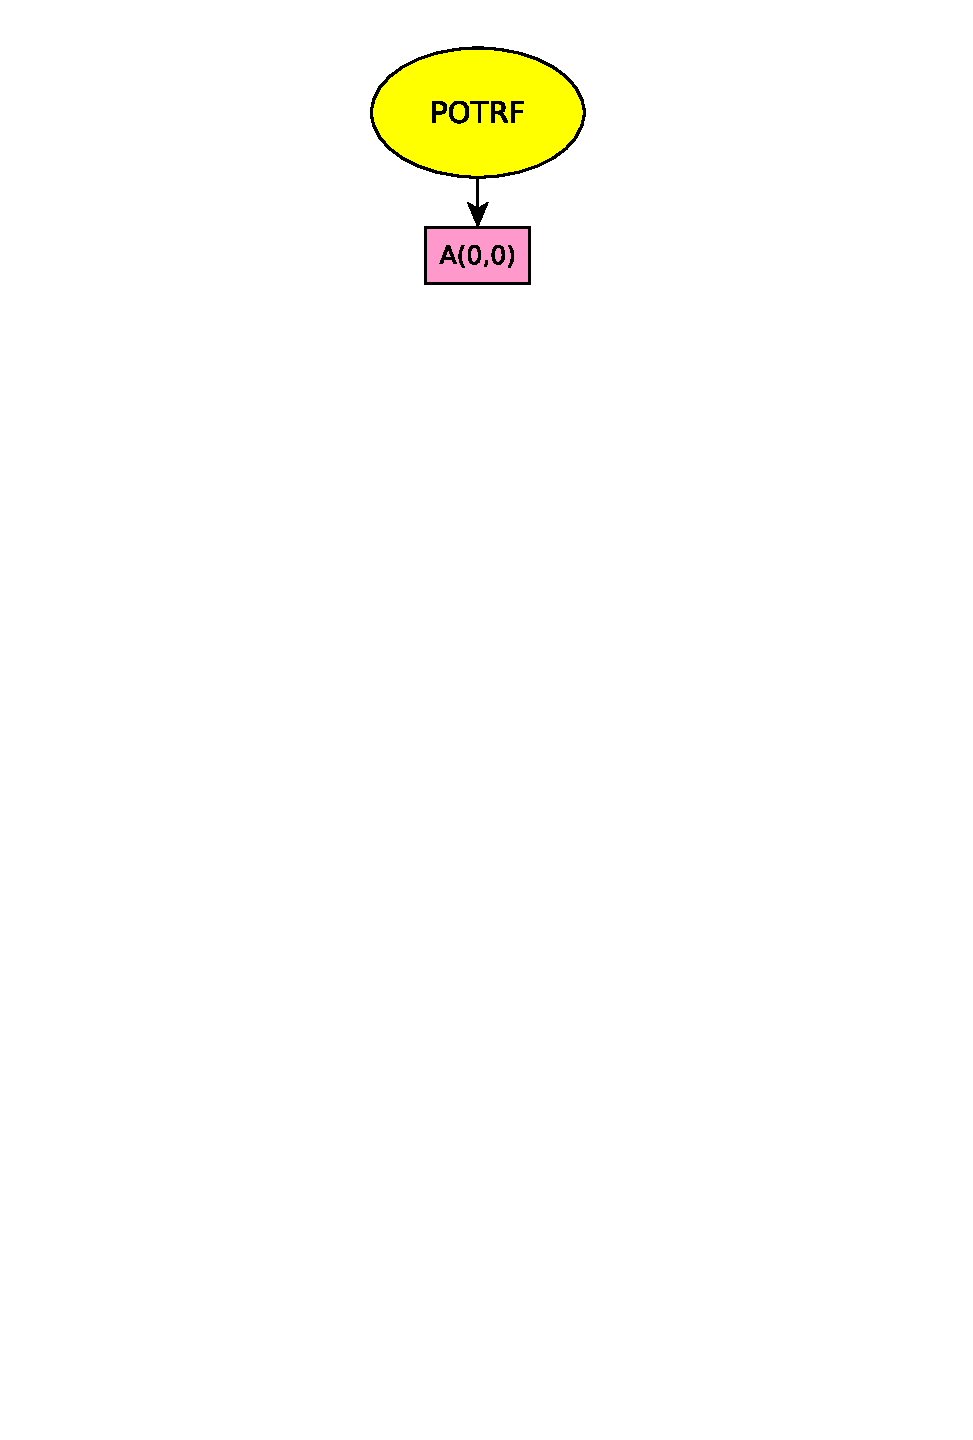
\includegraphics[width=0.9\textwidth]{graph/anim-dag/anim-1.pdf}%
  }%
  \only<2>{%
    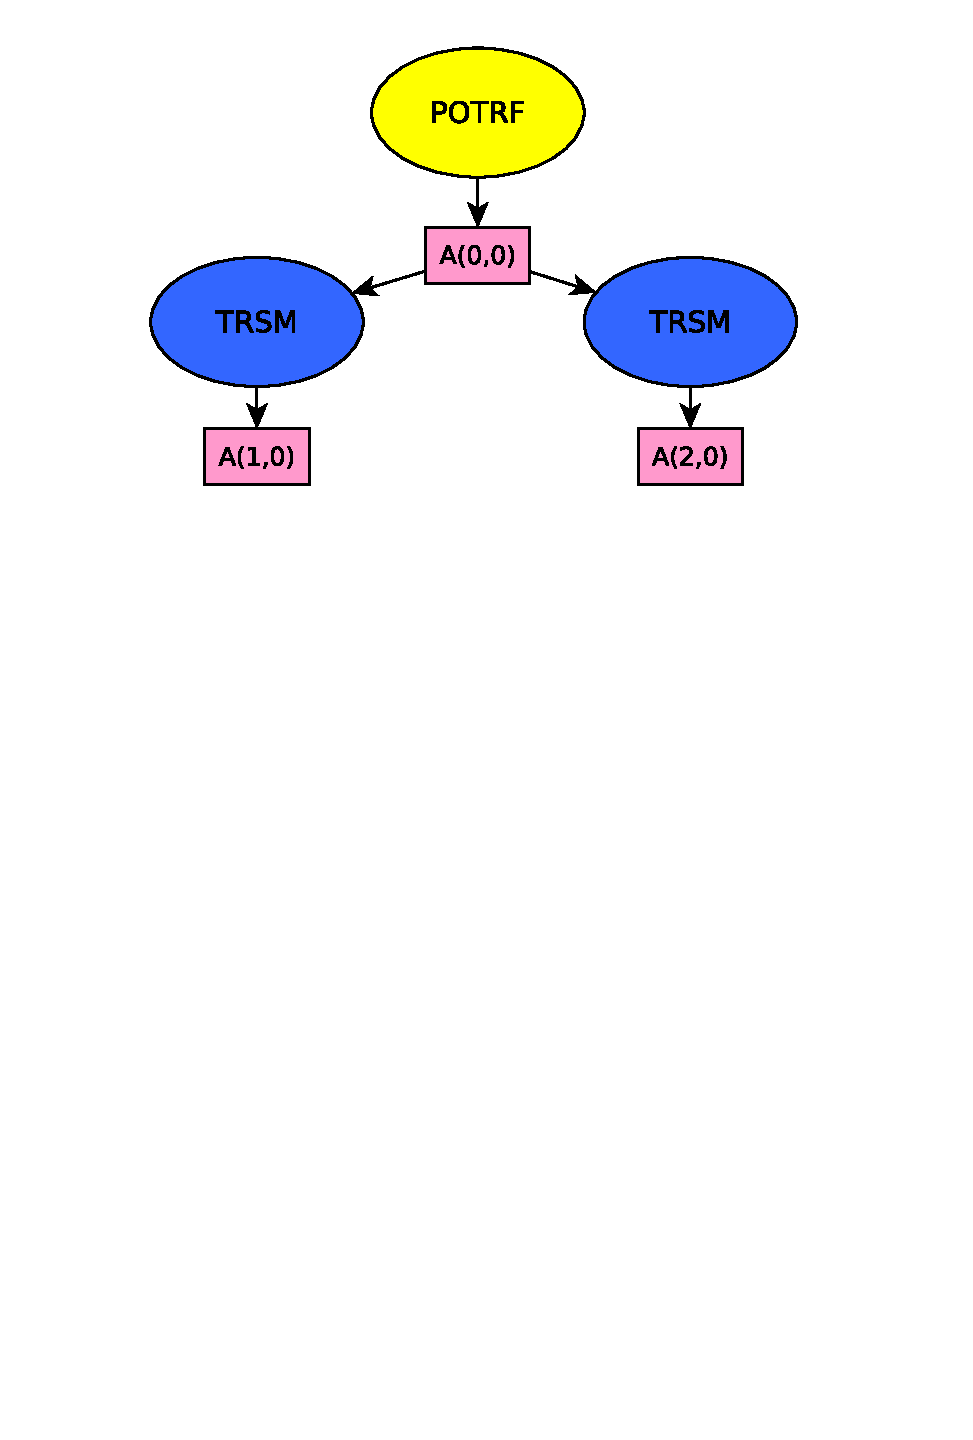
\includegraphics[width=0.9\textwidth]{graph/anim-dag/anim-2.pdf}%
  }%
  \only<3>{%
    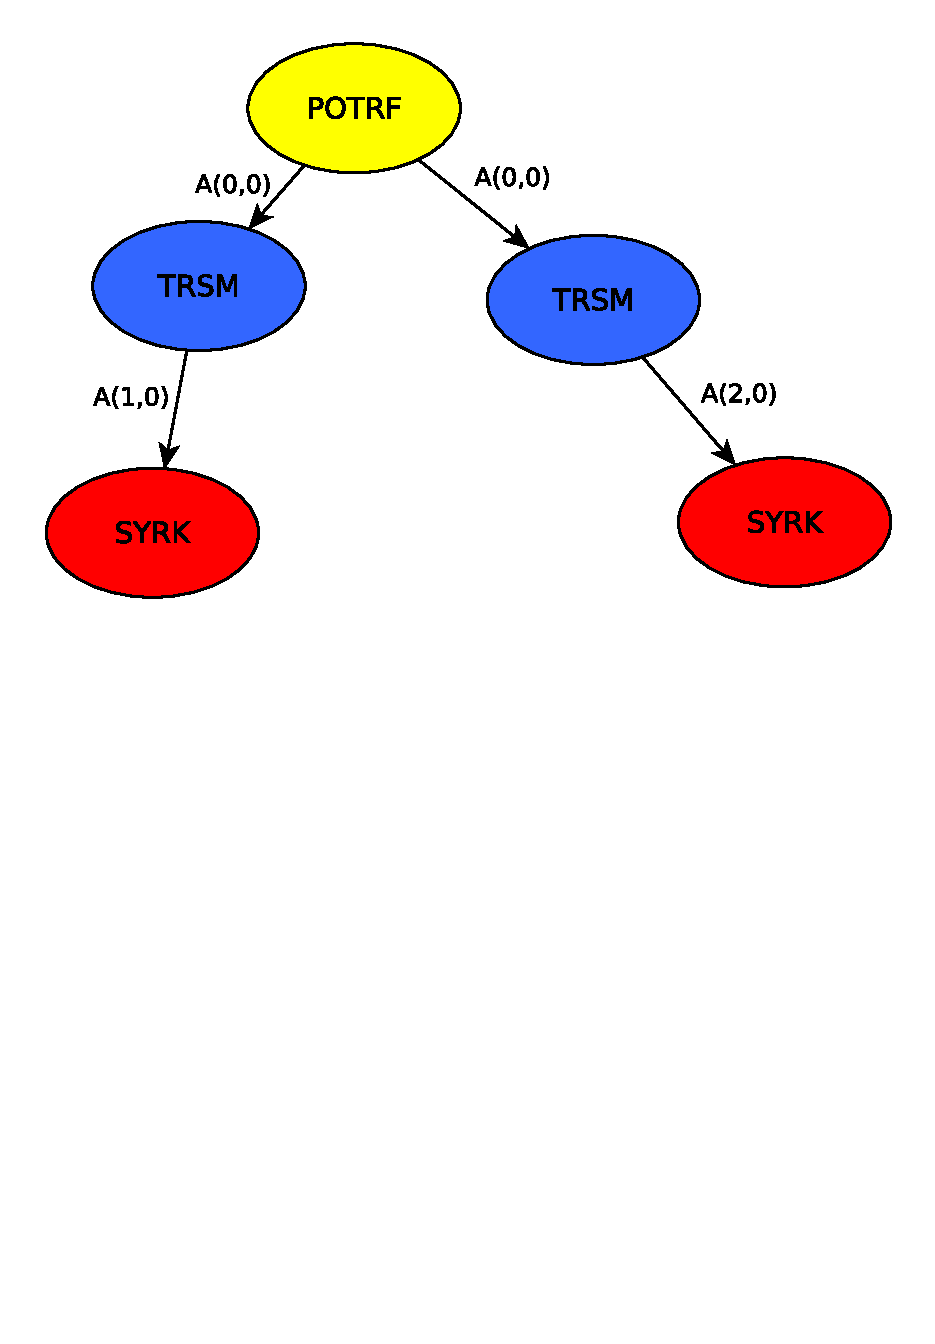
\includegraphics[width=0.9\textwidth]{graph/anim-dag/anim-3.pdf}%
  }%
  \only<4>{%
    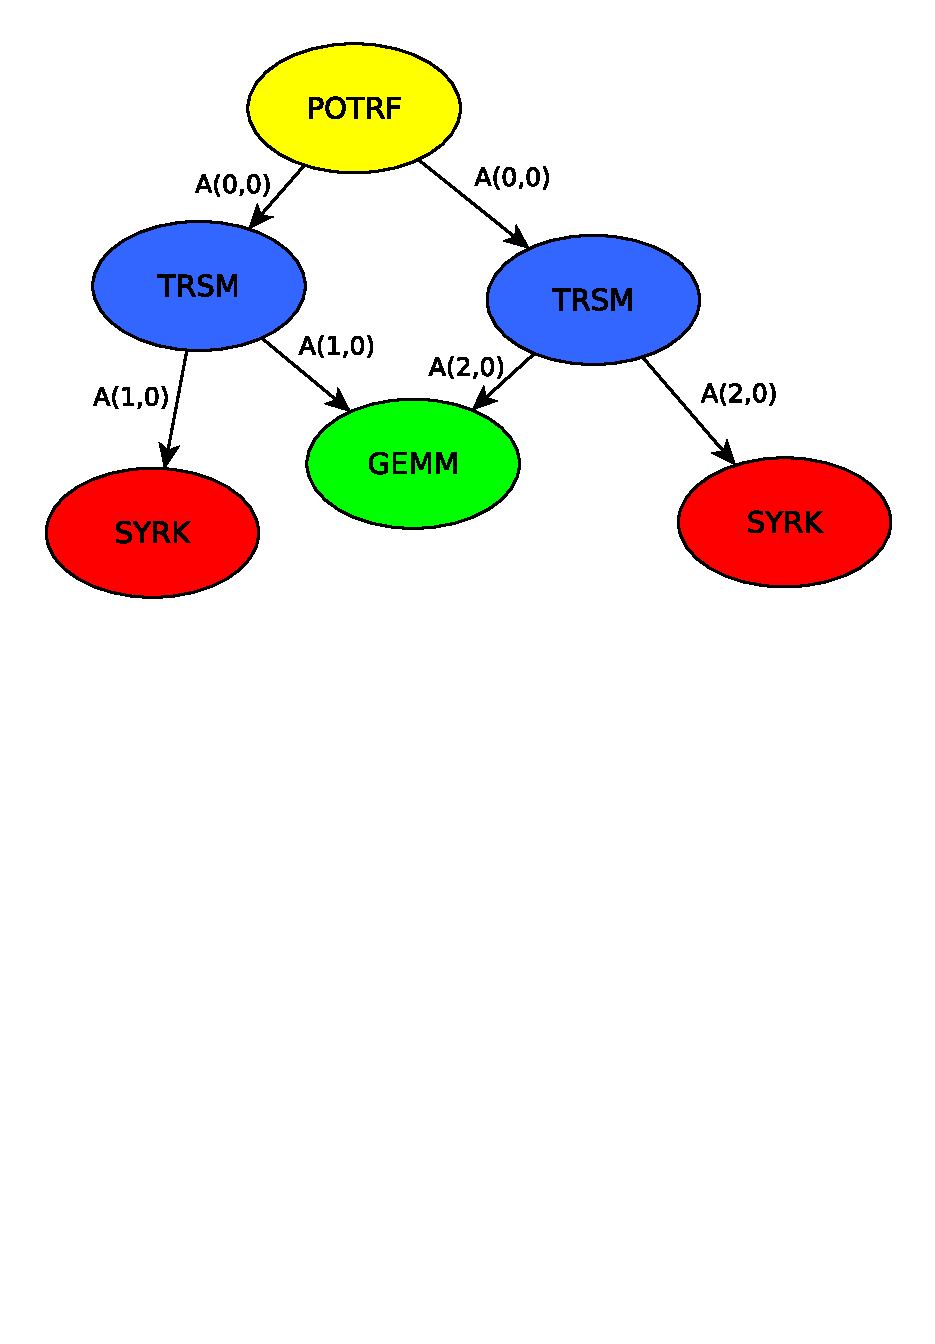
\includegraphics[width=0.9\textwidth]{graph/anim-dag/anim-4.pdf}%
  }%
  \only<5>{%
    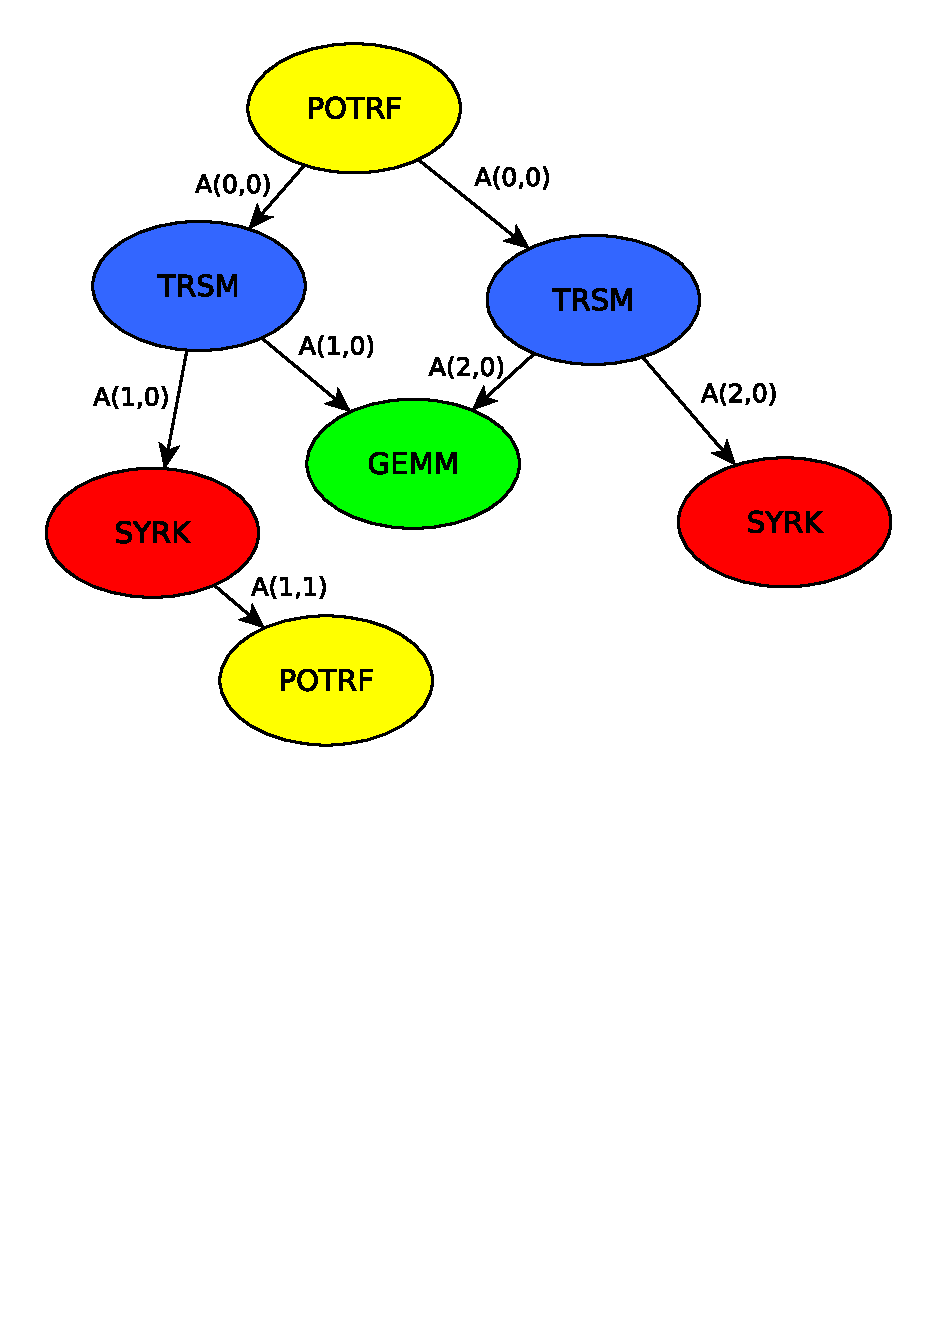
\includegraphics[width=0.9\textwidth]{graph/anim-dag/anim-5.pdf}%
  }%
  \only<6>{%
    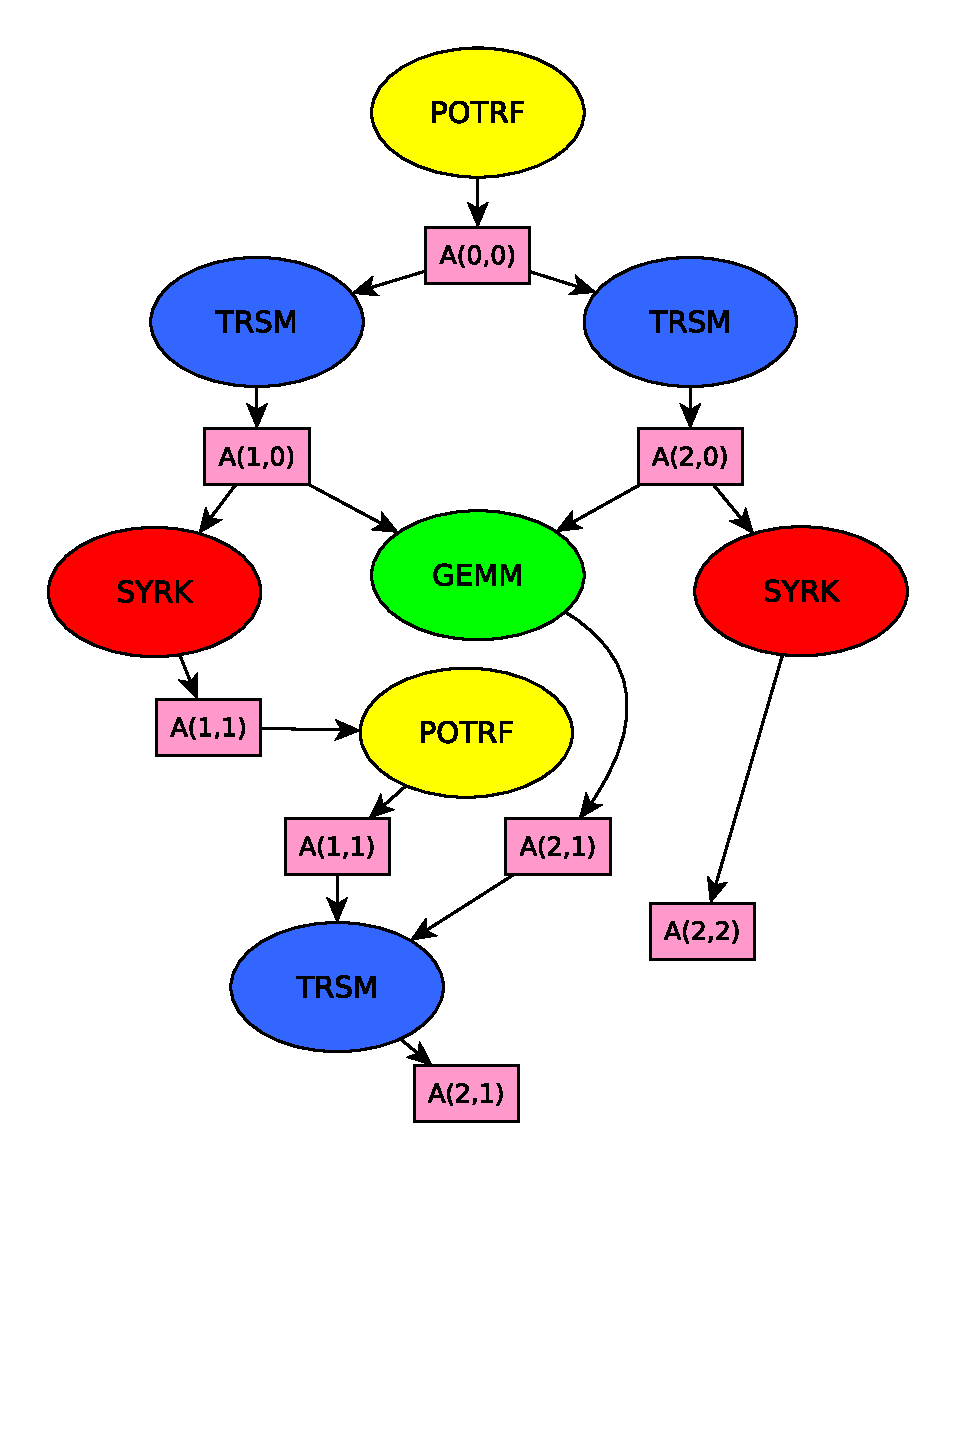
\includegraphics[width=0.9\textwidth]{graph/anim-dag/anim-6.pdf}%
  }%
  \only<7>{%
    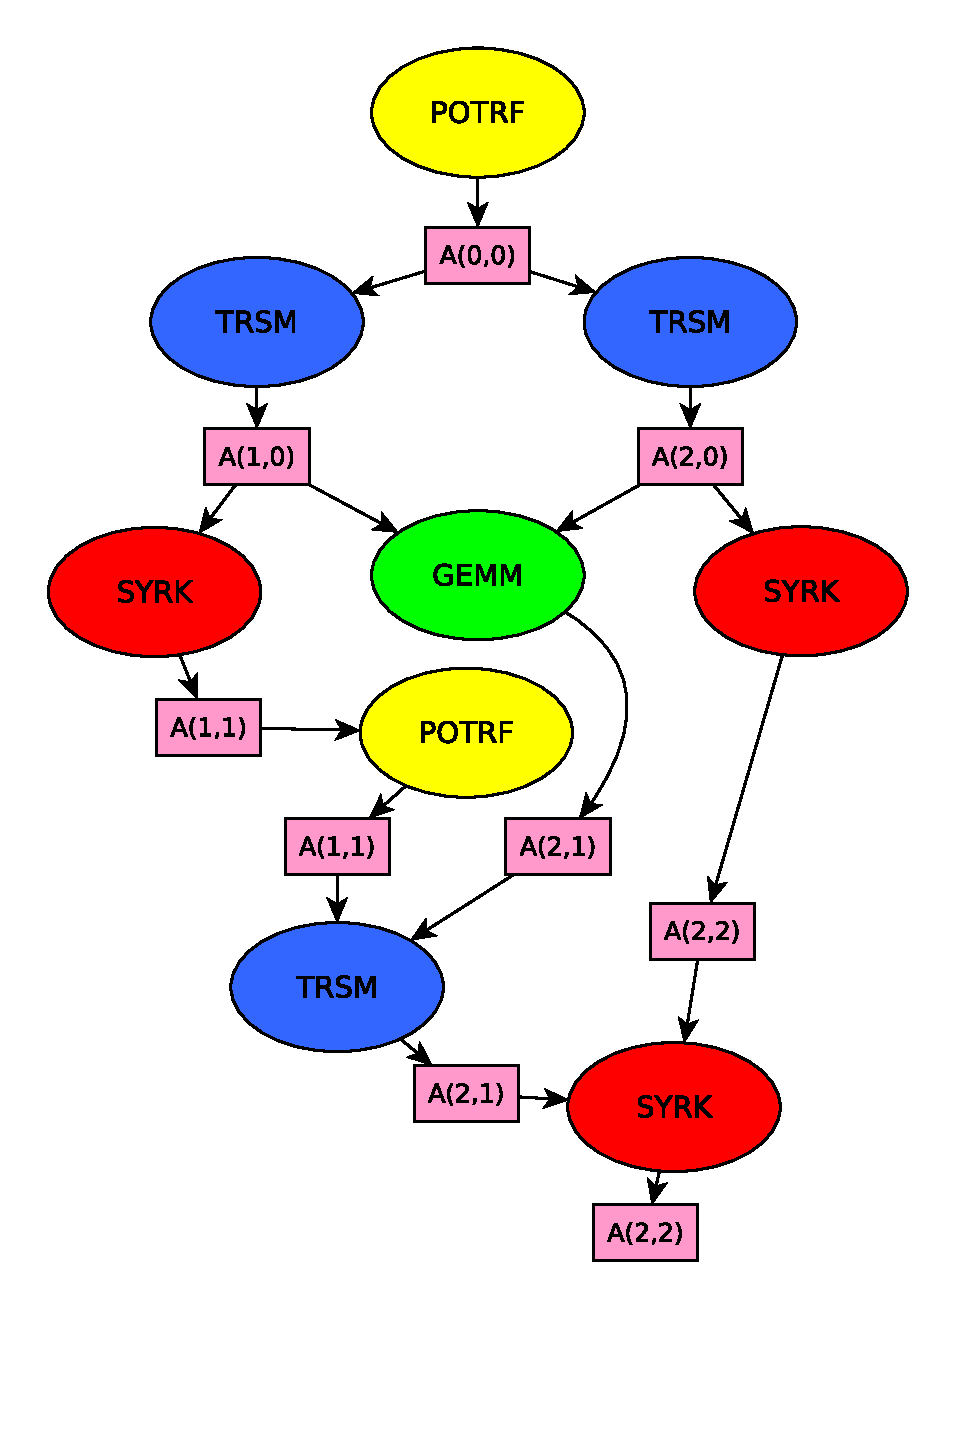
\includegraphics[width=0.9\textwidth]{graph/anim-dag/anim-7.pdf}%
  }%
  \only<8>{%
    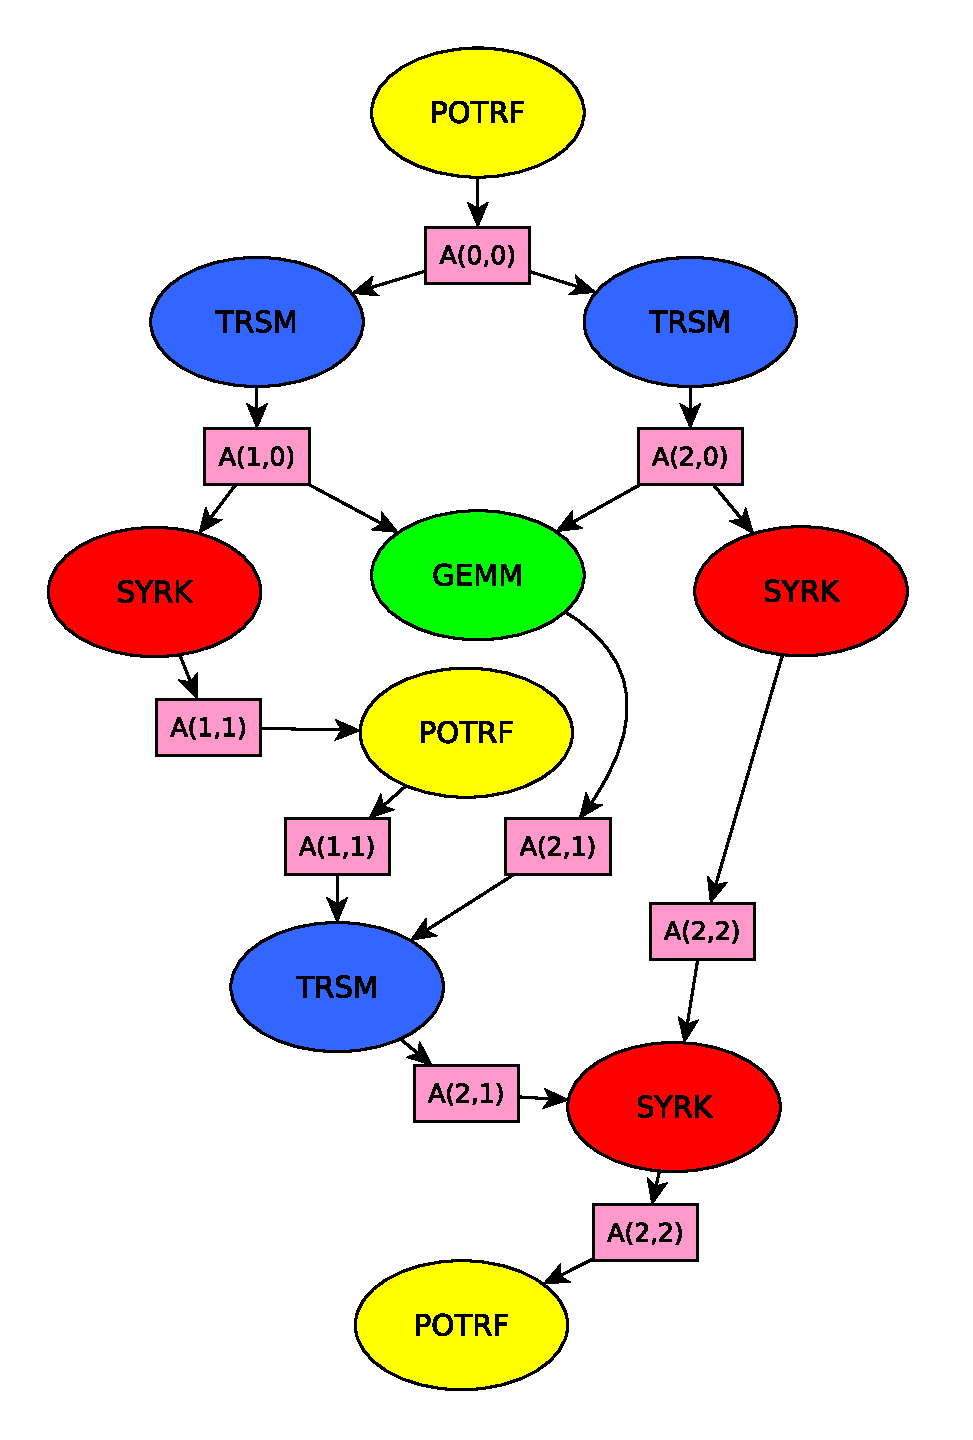
\includegraphics[width=0.9\textwidth]{graph/cholesky-dag-3-data.pdf}%
  }%
\end{figure}
\end{minipage}


\end{frame}


\begin{frame}
  \frametitle{Cholesky : performances brutes (32768, 512)}

  Évolution de la performance (Gflops) en fonction du nombre de cœurs.\\
  Exécution via libKOMP sur une machine à 192 cœurs.

\begin{figure}
  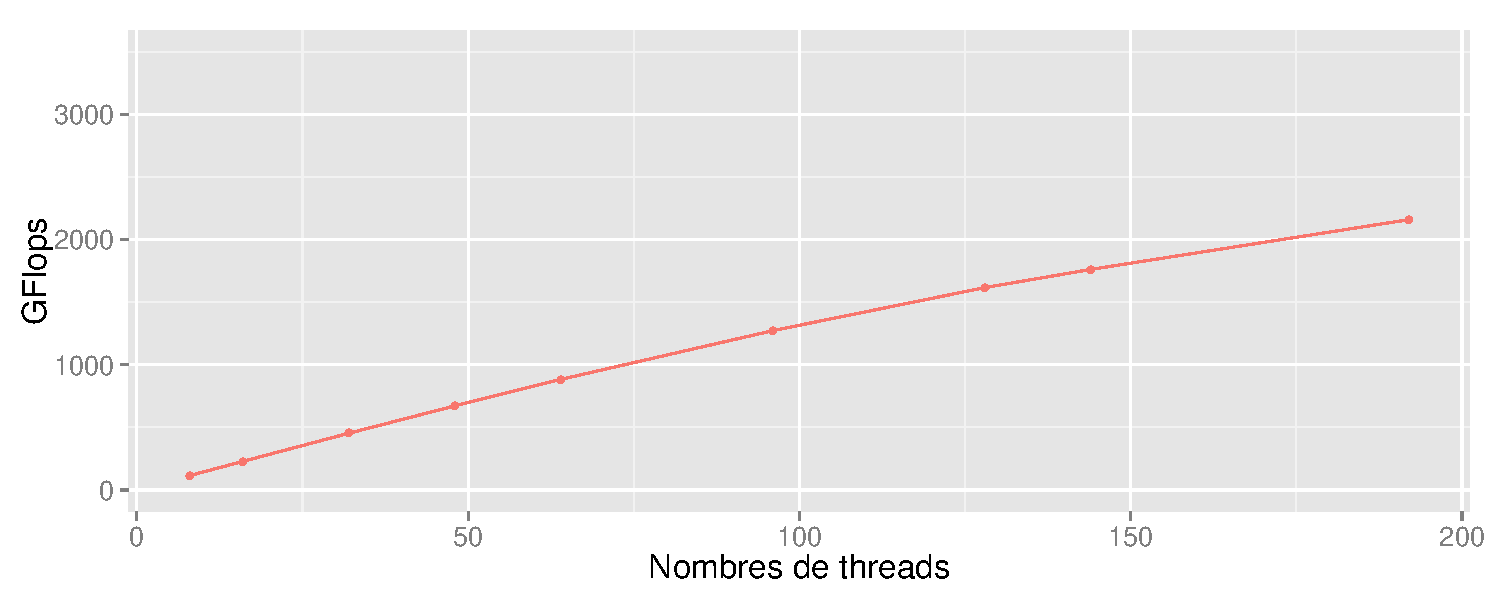
\includegraphics[width=\textwidth]{graph/graph_evolution_cholesky_32768_512.pdf}
\end{figure}
\uncover<2> {
  \begin{block}{Conclusions}
    Peu de conclusion à tirer : bon speedup jusqu'à ~70 cœurs, puis plateau potentiellement dû au parallélisme limité.
  \end{block}
}

\end{frame}

\begin{frame}
\frametitle{Cholesky : déroulement de l'application}

Aperçu d'un diagramme de Gantt sur 64 threads
\begin{figure}
  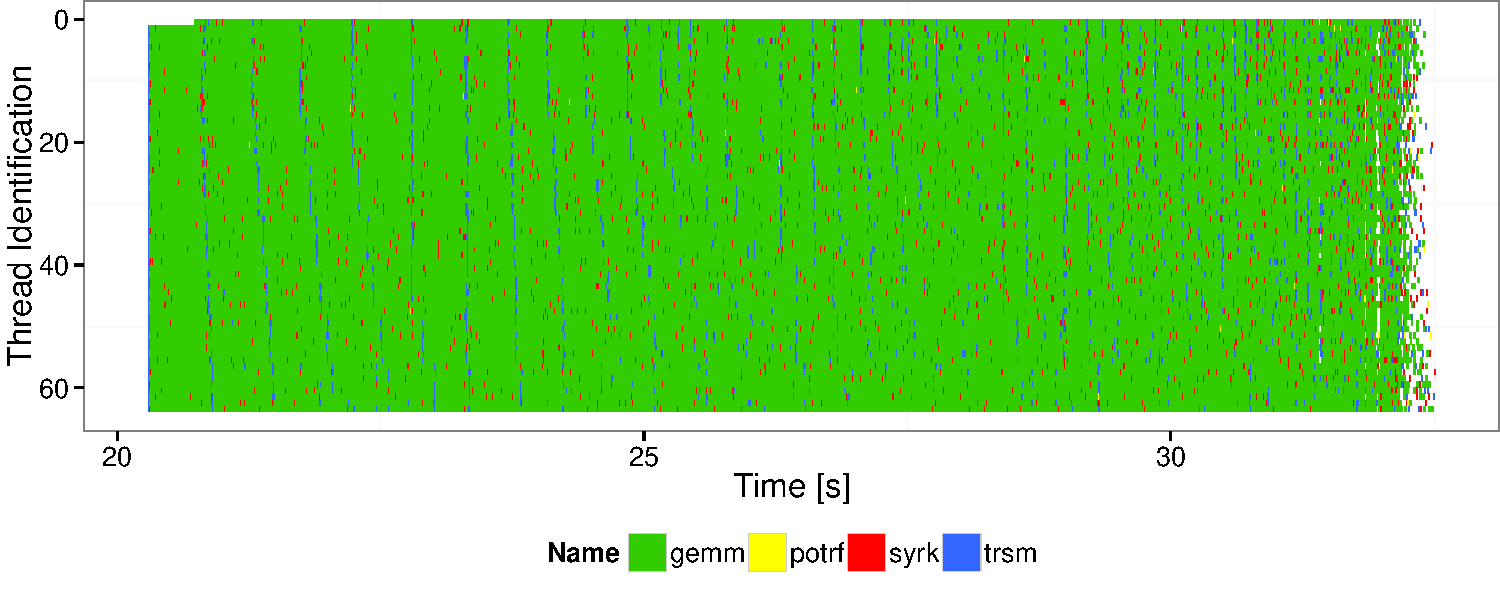
\includegraphics[width=\textwidth]{graph/gantt_32768_512.pdf}
\end{figure}
\uncover<2> {
  \begin{block}{Conclusions}
    Bonne utilisation des ressources, "trous" dûs à la forme du DAG sur la fin de l'exécution.
  \end{block}
}

\end{frame}

\begin{frame}
  \frametitle{Cholesky : comportement des différents types de tâches}
  \begin{figure}
    \only<1> {%
      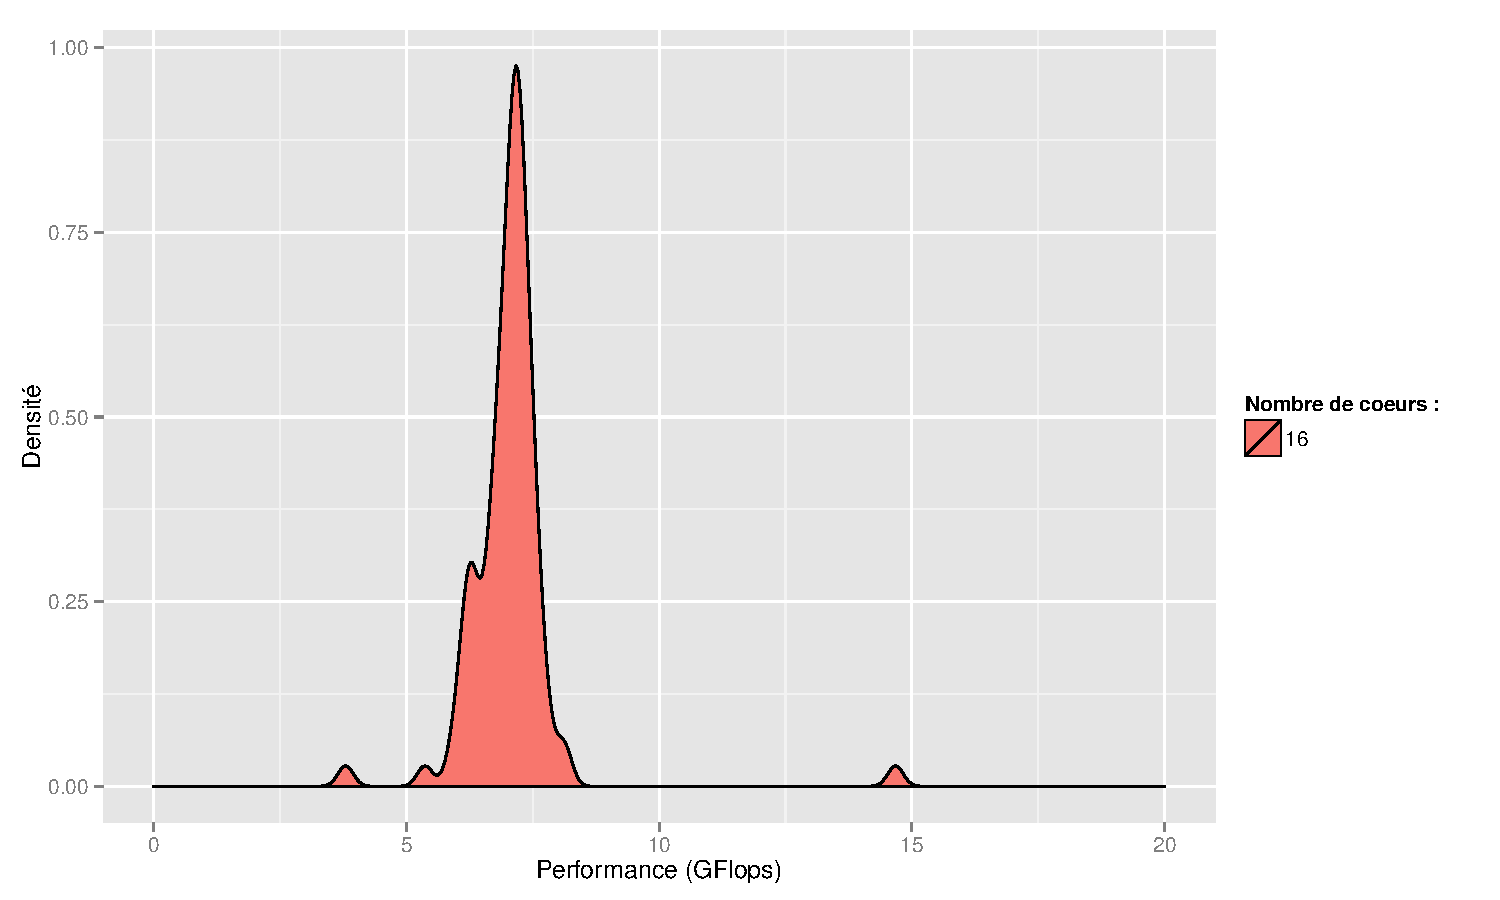
\includegraphics[width=0.8\textwidth]{graph/anim-distrib/graph_anim_distrib.pdf}%
    }%
    \only<2> {%
      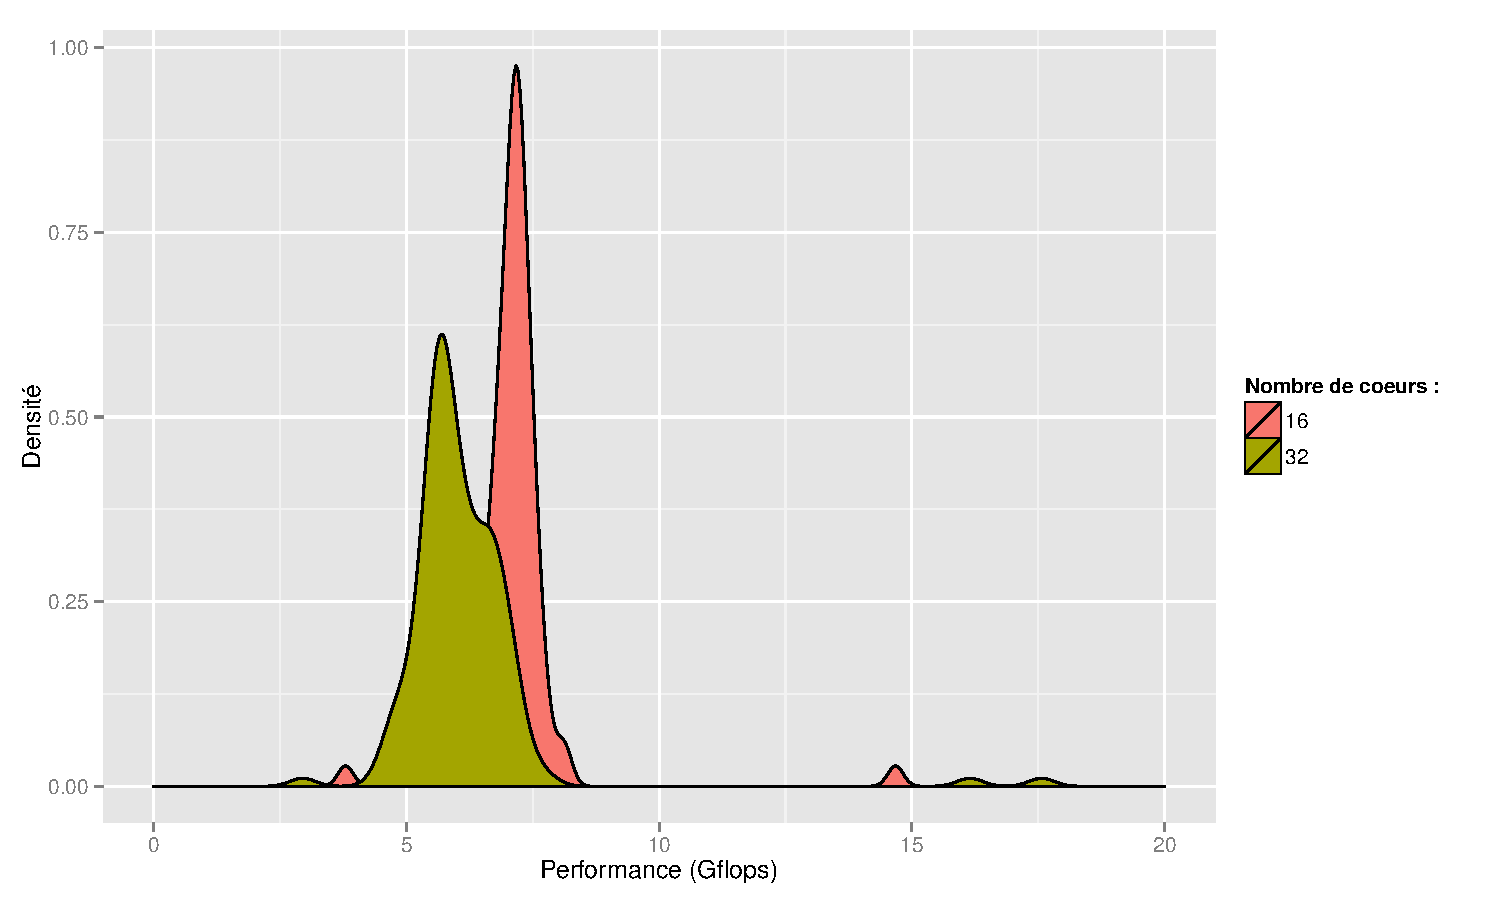
\includegraphics[width=0.8\textwidth]{graph/anim-distrib/graph_anim_distrib_1.pdf}%
    }%
    \only<3> {%
      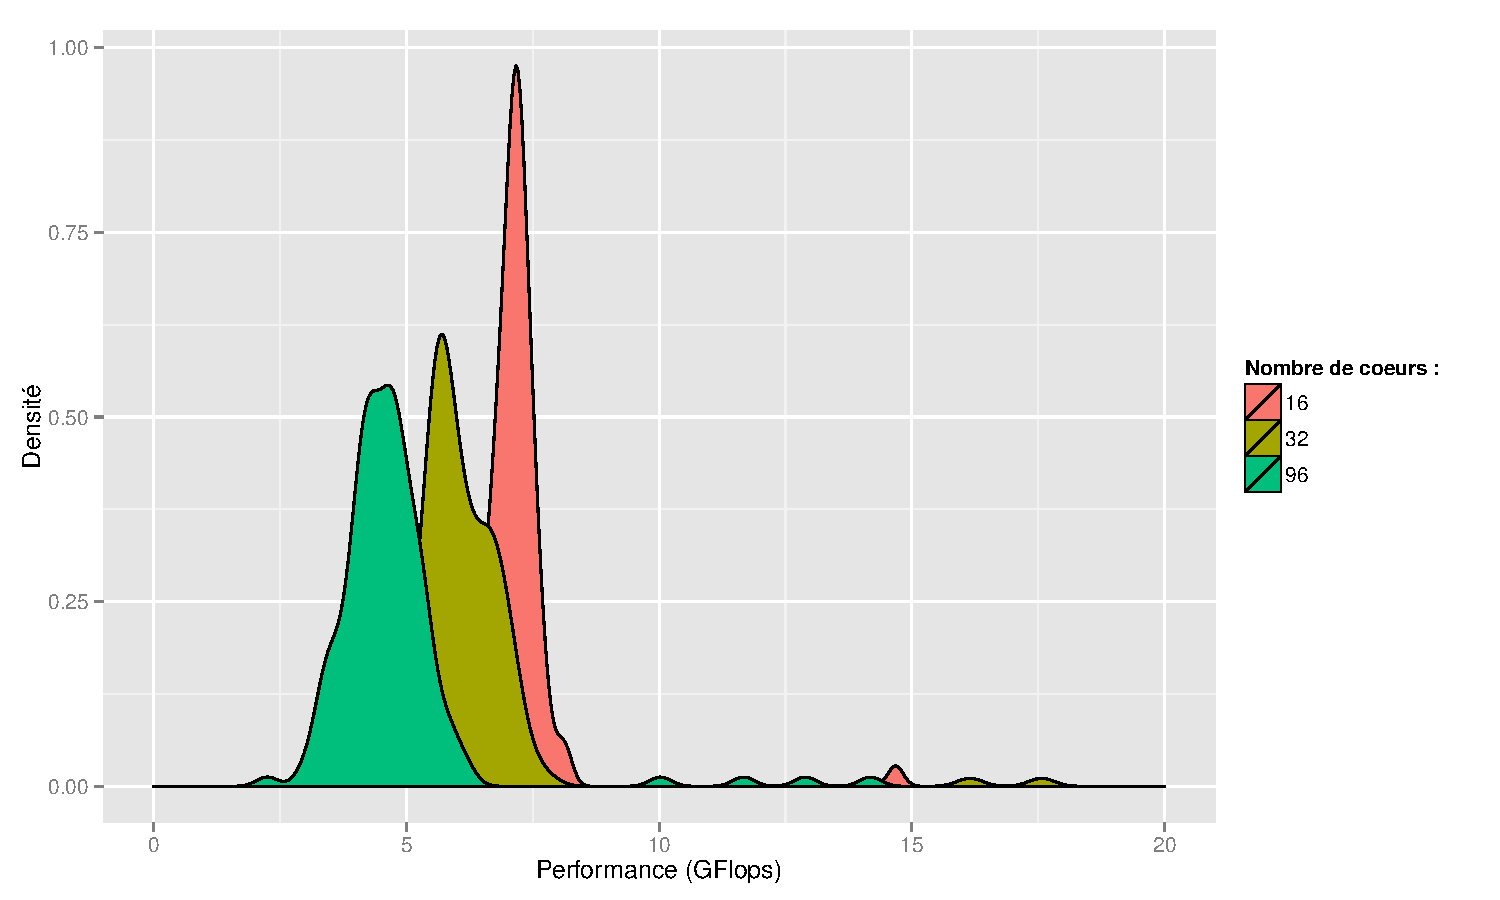
\includegraphics[width=0.8\textwidth]{graph/anim-distrib/graph_anim_distrib_2.pdf}%
    }%
    \only<4> {%
      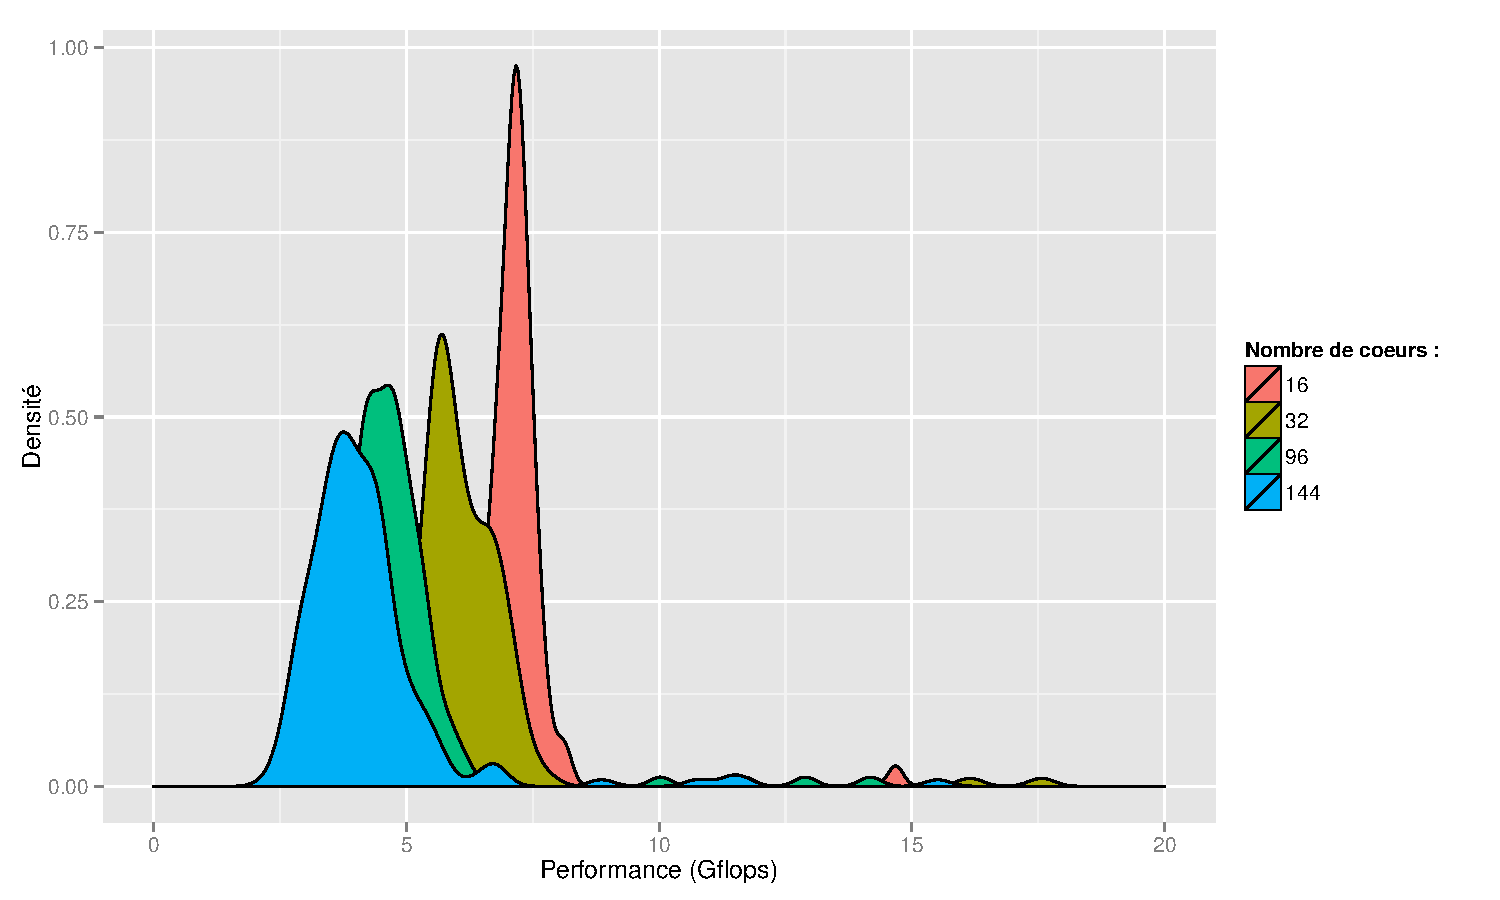
\includegraphics[width=0.8\textwidth]{graph/anim-distrib/graph_anim_distrib_3.pdf}%
    }%
    \only<5> {%
      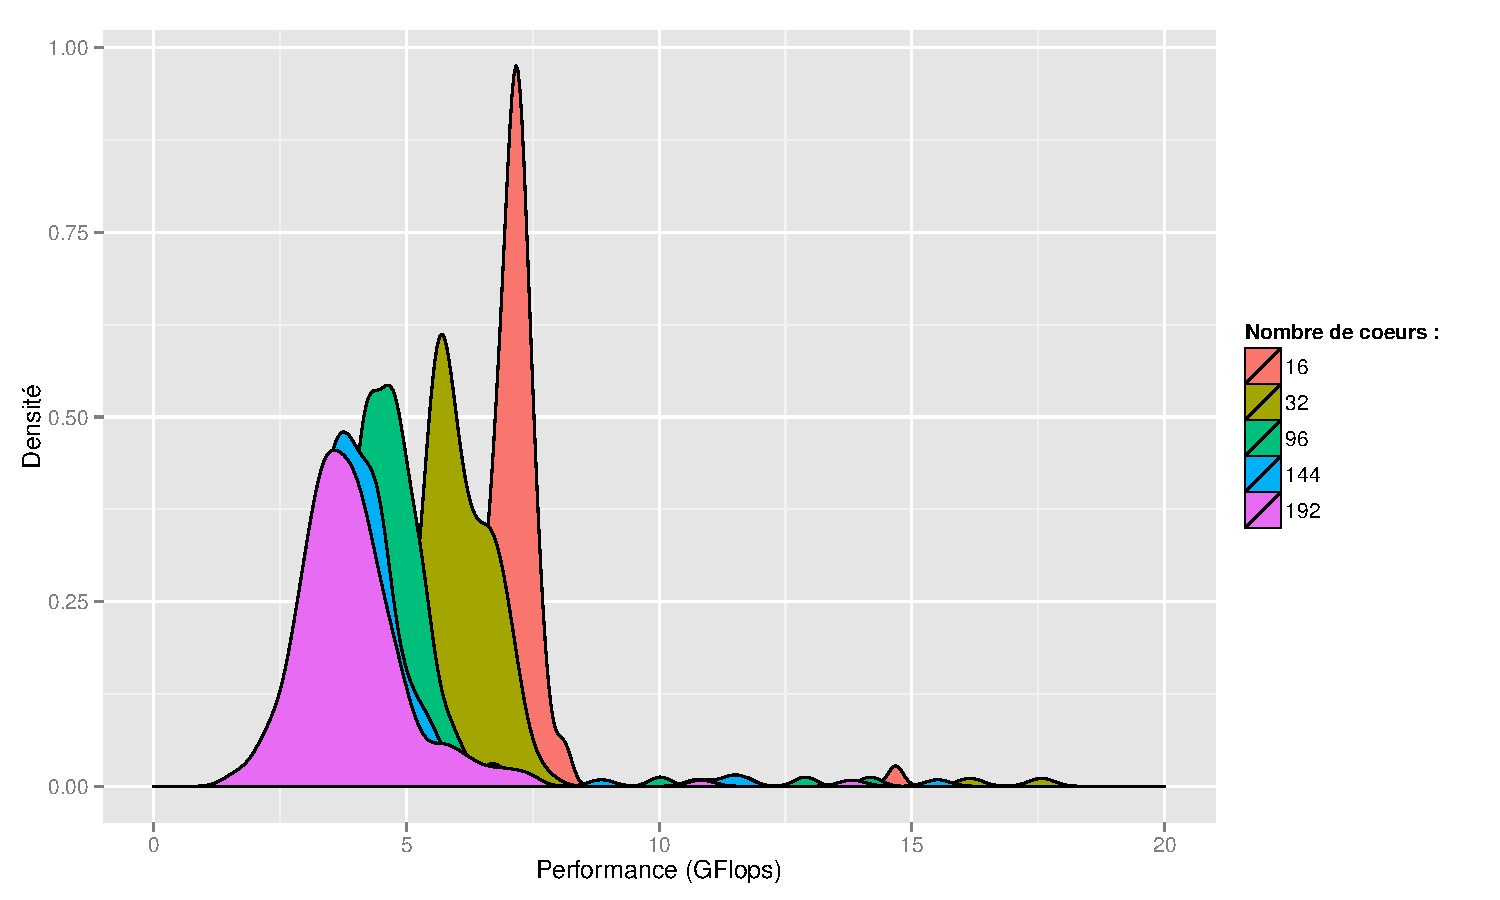
\includegraphics[width=0.8\textwidth]{graph/anim-distrib/graph_anim_distrib_4.pdf}%
    }%
    \only<6> {%
      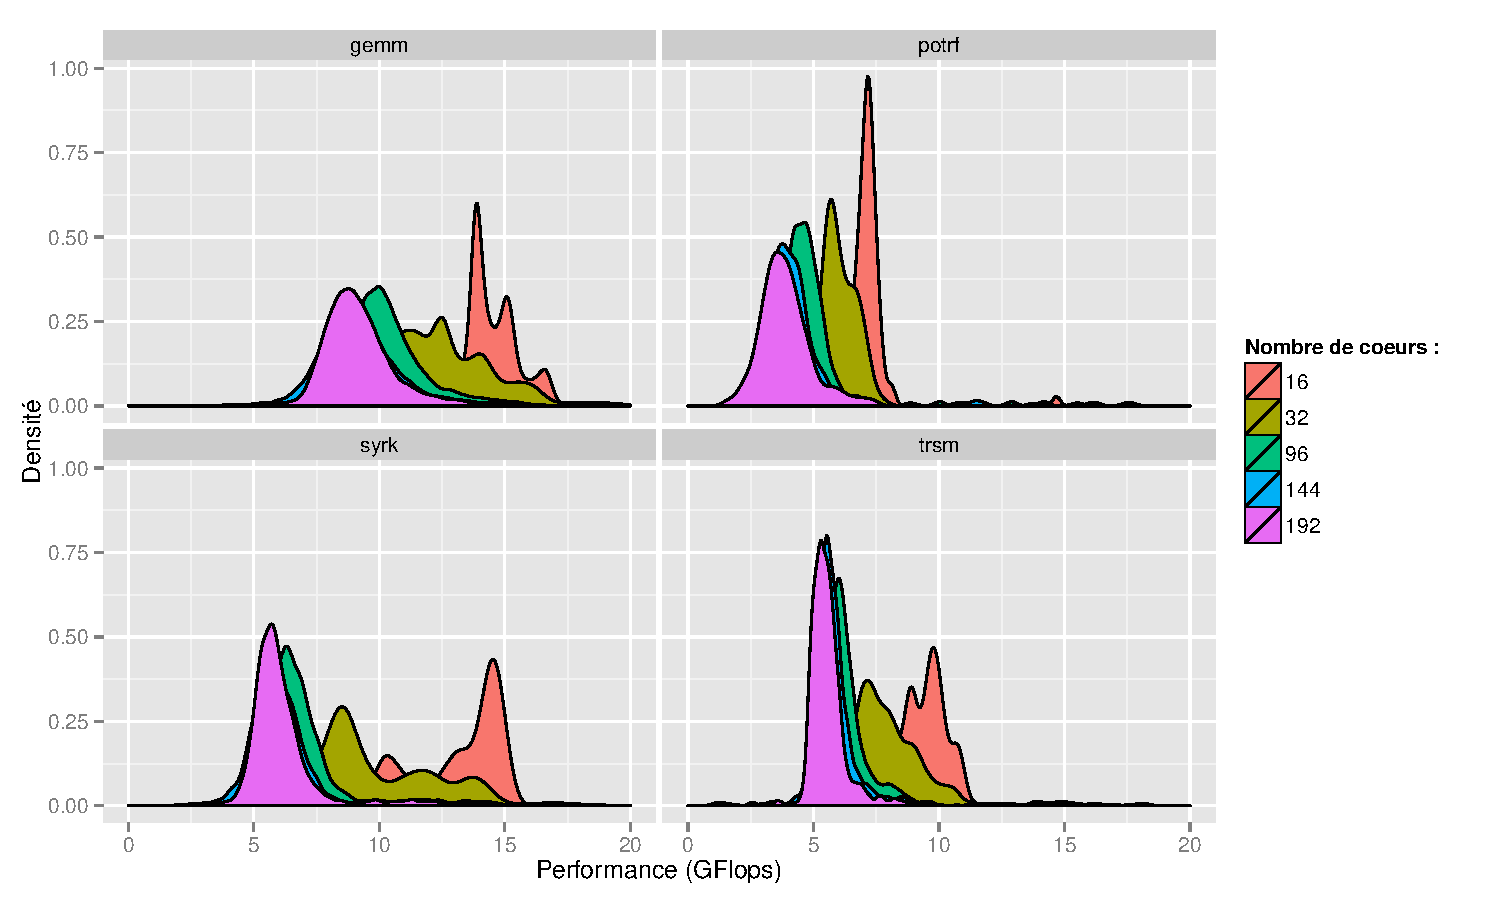
\includegraphics[width=0.8\textwidth]{graph/graph_distrib_overview.pdf}%
    }%

  \end{figure}
  \only<1-5> {
    Distribution des performances de chaque \potrf
  }
  \only<6> {
    \begin{block}{Conclusions}
      Nombre de threads qui augmente $=>$ diminution de la performance moyenne, augmentation de la variabilité.
    \end{block}
  }
\end{frame}


%TODO: T=#inst * cycle/#inst * 1/freq
%algo, vector,numa, hardware
\begin{frame}
  \frametitle{Source(s) des différences de performances}

  \begin{block}{Décomposition d'une tâche}
    $$ T_{total} = \overbrace{N_{instructions}}^\text{\uncover<2->{Algorithme}} * \underbrace{\frac{cycle}{N_{instructions}}}_\text{\uncover<4>{Vectorisation, localité des données}} * \overbrace{\frac{Secondes}{cycle}}^\text{\uncover<3->{Fréquence}} $$
  \end{block}

  \begin{block}{Leviers possibles}
    D'un point de vue support exécutif :
    \begin{itemize}
      \uncover<2->{
	\item Algorithme : donné en entrée
      }
      \uncover<3->{
	\item Fréquence : governor \textit{performance}
      }
      \uncover<4>{
	\item Vectorisation : dépendante du compilateur, fixe.
	\item \textbf{Localité des données : clé du problème.}
      }
    \end{itemize}
  \end{block}

\end{frame}

\begin{frame}
\frametitle{Localité des données : aperçu d'une machine NUMA}
%Texte : dire ce que ça veut dire NUMA, que les données sont partagées, décrire idchire
\begin{columns}[T,onlytextwidth]
  \column{0.42\textwidth}
  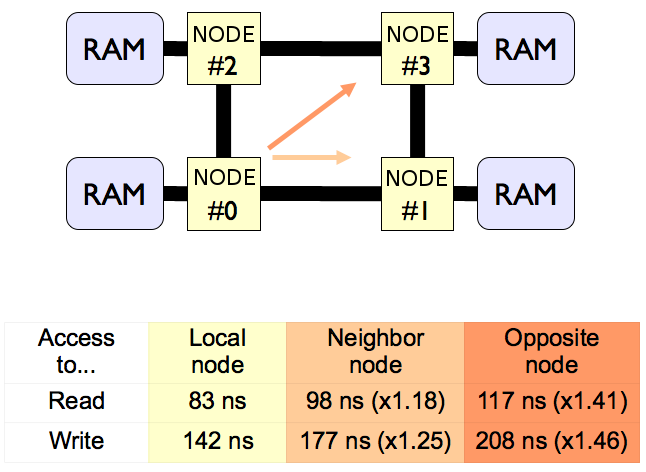
\includegraphics[scale=0.3]{graph/NUMA-latences}
  \column{0.40\textwidth}

  \begin{block}{Description}
    \begin{itemize}
      \item Mémoire partagée
      \item Machine = plusieurs nœuds
      \item Nœud = plusieurs cœurs + une sous partie de la RAM
    \end{itemize}
  \end{block}

\end{columns}
\begin{alertblock}{Conséquence principale}
  Le temps d'exécution d'une tâche dépend de son placement et du placement de ses données
\end{alertblock}

\end{frame}

\begin{frame}
  \frametitle{Bilan}

  \begin{block}{Observations (outils "classiques")}
    \begin{itemize}
      \item Performances brutes
      \item Utilisation des resources (Gantt)
      \item Analyse statistique
    \end{itemize}
    => Mise en évidence d'un problème
  \end{block}
\end{frame}

\begin{frame}
  \frametitle{Méthodologie pour l'amélioration d'une application}
  \begin{minipage}[t]{0.36\linewidth}
    \begin{block}{Problématiques}
      \begin{itemize}
	\uncover<2->{
	  \item Identifier les facteurs responsables
	  \item Chiffrer leur impact
	}
	\only<3-4>{
	  \item Diminuer l'impact de ces facteurs
	}
	\only<4>{
	  \item Peut on prévoir les performances ?
	}
	\only<5>{
	  \transparent{0.5}{
	  \item Diminuer l'impact de ces facteurs
	  \item Peut on prévoir les performances ?
	  }
	}
      \end{itemize}
    \end{block}
  \end{minipage}
      \hfill
  \begin{minipage}[t]{0.60\linewidth}
    \begin{figure}
      \only<1> {%
	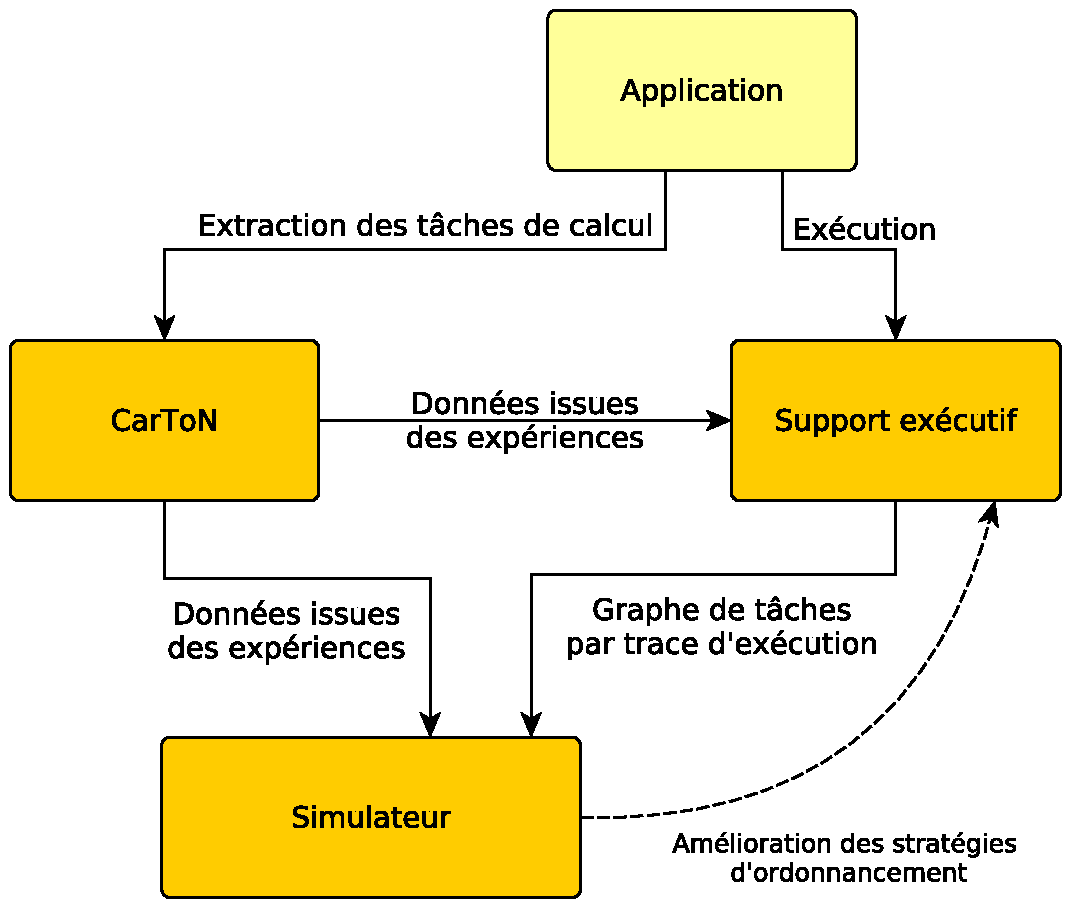
\includegraphics[width=\textwidth]{graph/big_picture.pdf}%
      }%
      \only<2,5> {%
	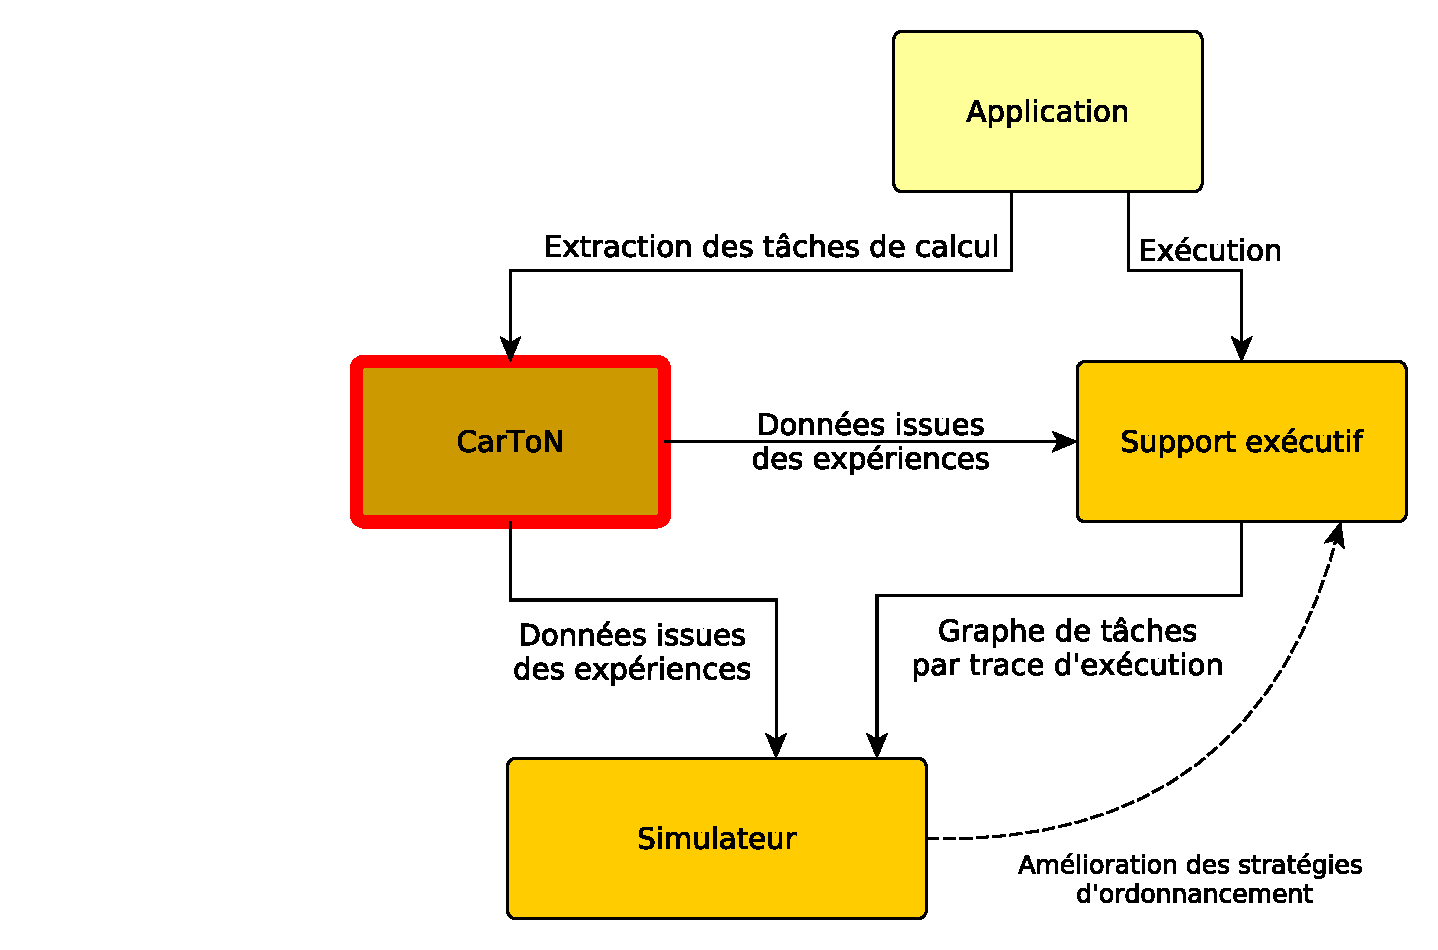
\includegraphics[width=\textwidth]{graph/big_picture-part1.pdf}%
      }%
      \only<3> {%
	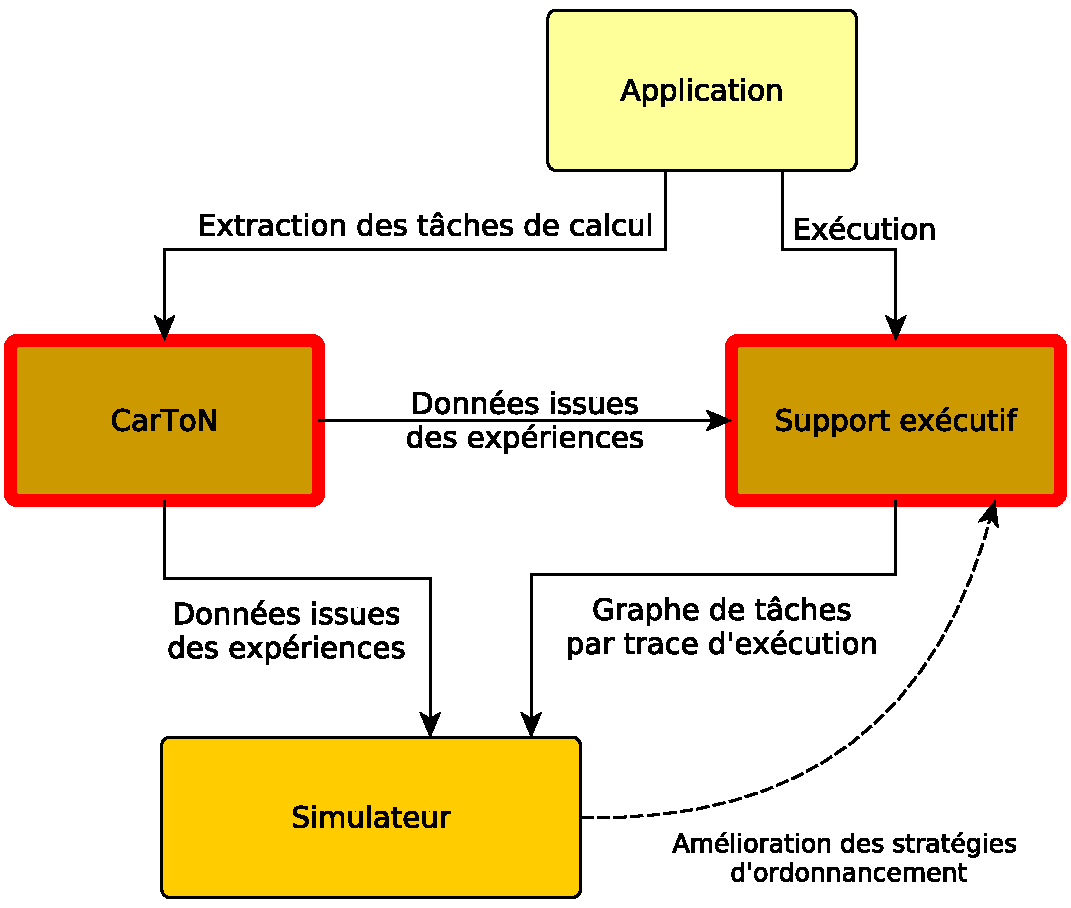
\includegraphics[width=\textwidth]{graph/big_picture-part1-2.pdf}%
      }%
      \only<4> {%
	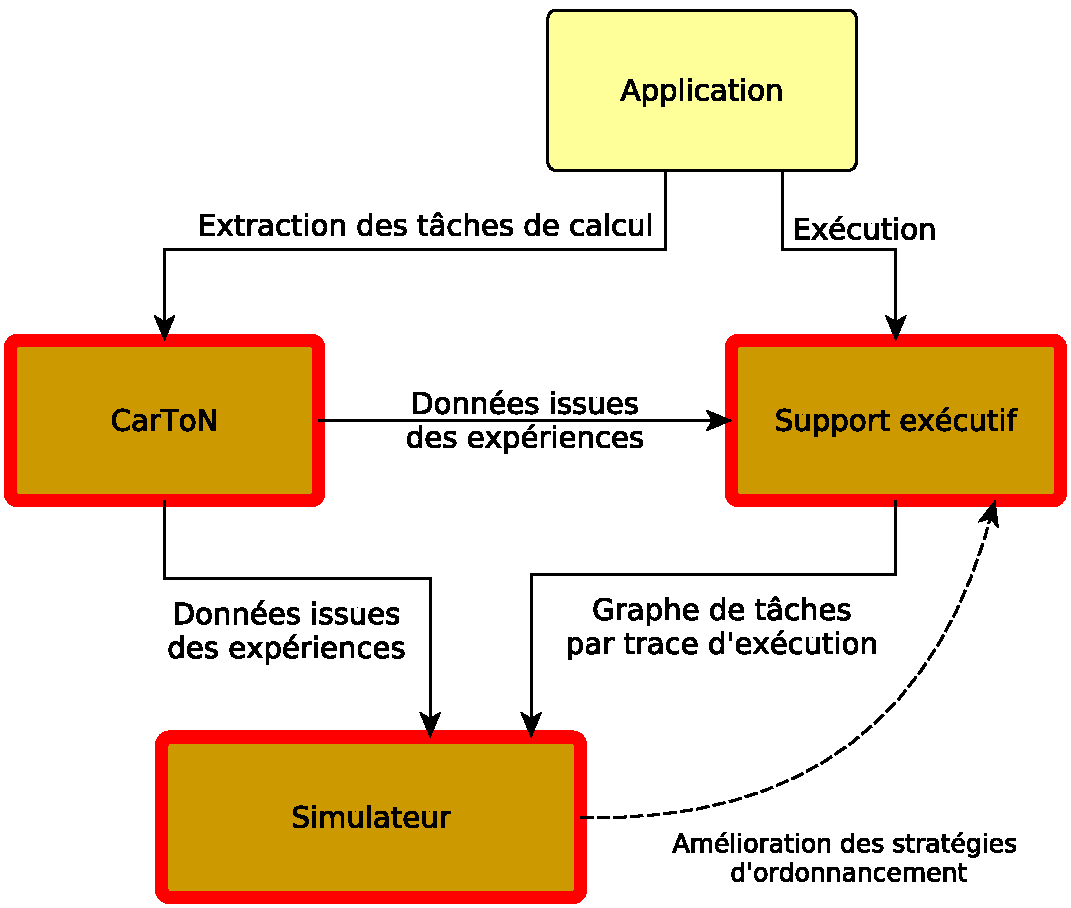
\includegraphics[width=\textwidth]{graph/big_picture-part1-3.pdf}%
      }%
    \end{figure}
  \end{minipage}
\end{frame}

\begin{frame}
\frametitle{Caractérisation des noyaux de Cholesky}

\begin{block}{Objectif}
  Analyser le comportement des quatre noyaux de l'application (\potrf, \trsm, \syrk, \gemm).

  Conditions d'expérience :
  \begin{itemize}
    \item exécutions sur des données \emph{indépendantes}
    \item placement des données (locales, distantes)
    \item charge de la machine (nombre d'exécutions concurrentes)
  \end{itemize}
\end{block}

\end{frame}




\begin{frame}
  \frametitle{Quel outil pour notre besoin ?}

  Ce que l'on cherche à faire~:
  \begin{itemize}
    \item exécution de portions de code arbitraire
    \item connaissance et contrôle sur le placement des données manipulées
    \item intéractions entre différentes portions de codes (coéxécution)
    \item rejeu et observation
  \end{itemize}

  Ressources existantes~:
  \begin{itemize}
    \item Benchmarks, microbenchmarks en quantité

      STREAM, EPCC, NAS, ...

    \item Utilisant du code utilisateur arbitraire

      BOAST : autotuning de noyaux applicatifs.
  \end{itemize}

  \textbf{Pas d'outil existant répondant à notre besoin précis !}

\end{frame}

\begin{frame}
  \frametitle{CarToN : Characterization Tool for NUMA architectures}

  \begin{block}{Objectifs et motivations}
    \begin{itemize}
      \item Observer et comprendre le comportement d'un noyau applicatif arbitraire
      %\item Pas (peu) d'interférence liée à l'exécution
    \end{itemize}
  \end{block}

  \begin{block}{Éléments de base}
    Un \textbf{scénario} décrivant :
    \begin{itemize}
      \item Données (ex: matrice A, B)
      \item Actions (ex: B=A+B)
      \item Paramètres à observer (ex: flops, cache miss, ...)
    \end{itemize}
  \end{block}
\end{frame}

\begin{frame}[fragile]
\frametitle{Exemple : exécution de N \gemm indépendants}

\hspace{0.1cm}
\begin{minipage}[t]{0.38\linewidth}
  Déclaration des données
  \begin{lstlisting}[language=yaml]
data:
  size:
    type: int
    value: 256
  a<i>:
    i: [0, N, 1]
    mapping: i
    type: double*
  b<i>:
    i: [0, N, 1]
    mapping: i
    type: double*
  c<i>:
    i: [0, N, 1]
    mapping: i
    type: double*
  \end{lstlisting}
\begin{uncoverenv}<3->
  Paramètres à observer
  \begin{lstlisting}[language=yaml]
watchers:
- name: flops_dgemm
  params:
  - size
  kernels:
  - dgemm
  \end{lstlisting}
\end{uncoverenv}
\end{minipage}
\hspace{0.3cm}
\begin{uncoverenv}<2->
\begin{minipage}[t]{0.54\linewidth}
  Déclaration des actions
  \begin{lstlisting}[language=yaml]
actions:
- for:
  var: i
  limits: [0, N, 1]
  actions:
  - for:
    var: name
    values: ["a", "b", "c"]
    actions:
    - kernel: init_blas_bloc
      core: <i>
      params: "<name><i>", "size"
- kernel: barrier
- for:
  var: i
  limits: [0, N, 1]
  actions:
  - kernel: dgemm
    core: <i>
    repeat: '50'
    params: ["a<i>", "b<i>", "c<i>", "size"]
  \end{lstlisting}
\end{minipage}
\end{uncoverenv}

\end{frame}

\begin{frame}
  \frametitle{Matériel}

  \begin{block}{idchire (2012)}
    Machine LIG
    \begin{itemize}
      \item Intel Xeon E5-4640 @ 2.4 GHz, Sandy Bridge
      \item 24 nœuds NUMA, 8 cœurs par nœud, 192 cœurs.
      \item Cache L3 : 20 Mo
    \end{itemize}
  \end{block}

  \begin{block}{brunch (2016)}
    Machine LIP-ENS de Lyon, plus récente, et topologie plus simple :
    \begin{itemize}
      \item Intel Xeon E7-8890 @ 2.2 GHz, Broadwell
      \item 4 nœuds NUMA, 24 cœurs par nœud, 96 cœurs
      \item Cache L3 : 60 Mo (similaire à idchire, 2.5 Mo par cœur)
    \end{itemize}
  \end{block}

\end{frame}



\begin{frame}
\frametitle{Application aux noyaux de Cholesky}

Performance en fonction du nombre d'exécutions concurrentes (données locales)

Taille des matrices manipulées : 256x256
\begin{figure}
  \centering
  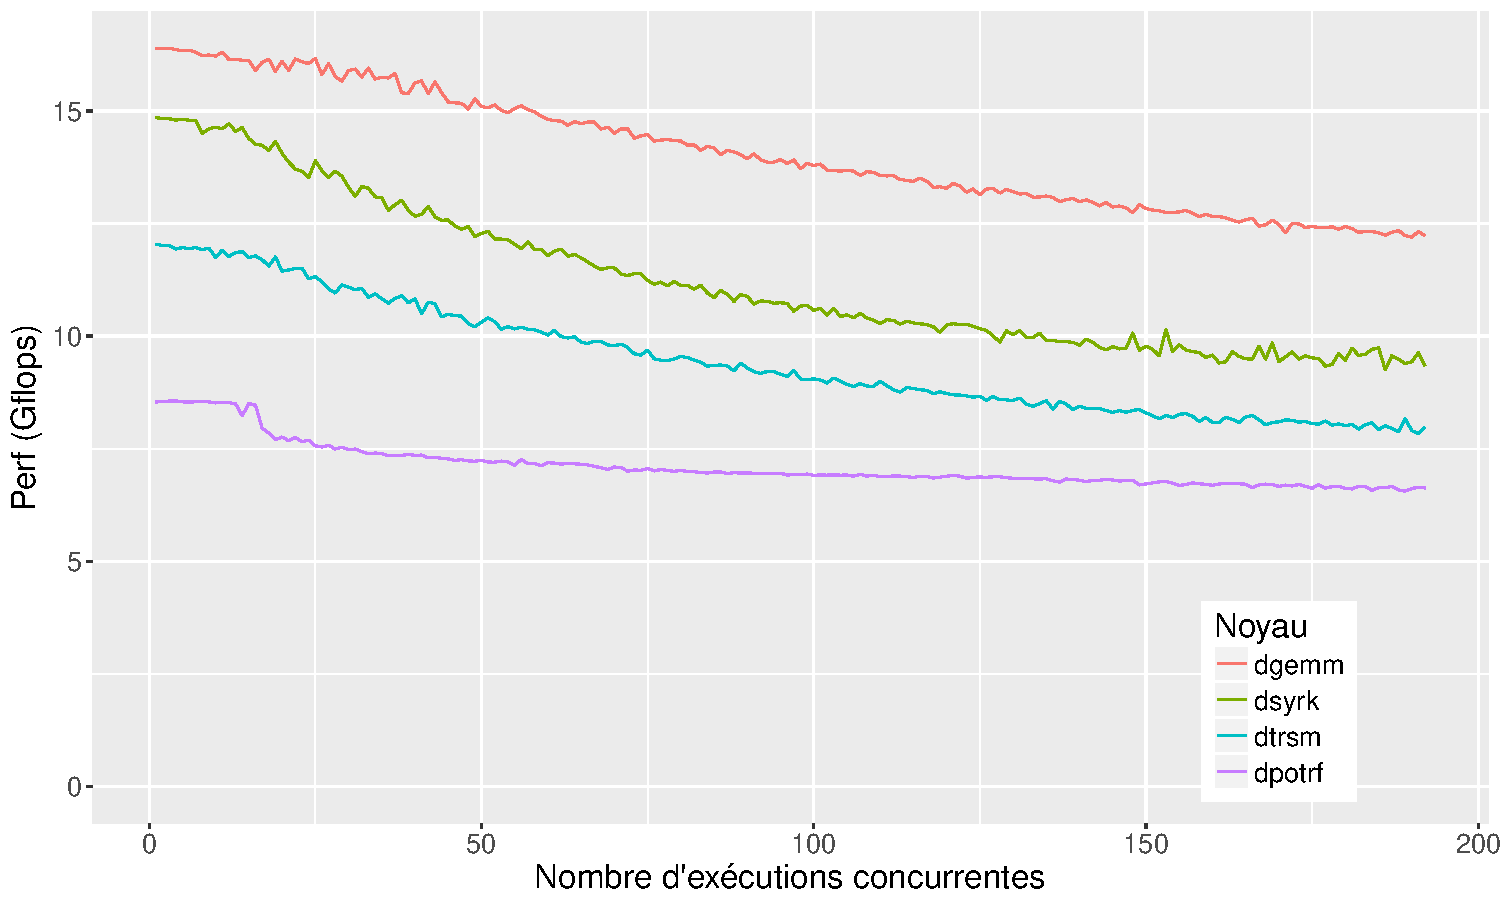
\includegraphics[width=0.85\textwidth]{graph/kernel_256_local_idchire.pdf}
\end{figure}

\end{frame}

\begin{frame}
\frametitle{Application aux noyaux de Cholesky}

Impact de la localité pour \gemm (512x512), en fonction du nombre d'exécutions concurrentes.

\begin{figure}
  \centering
  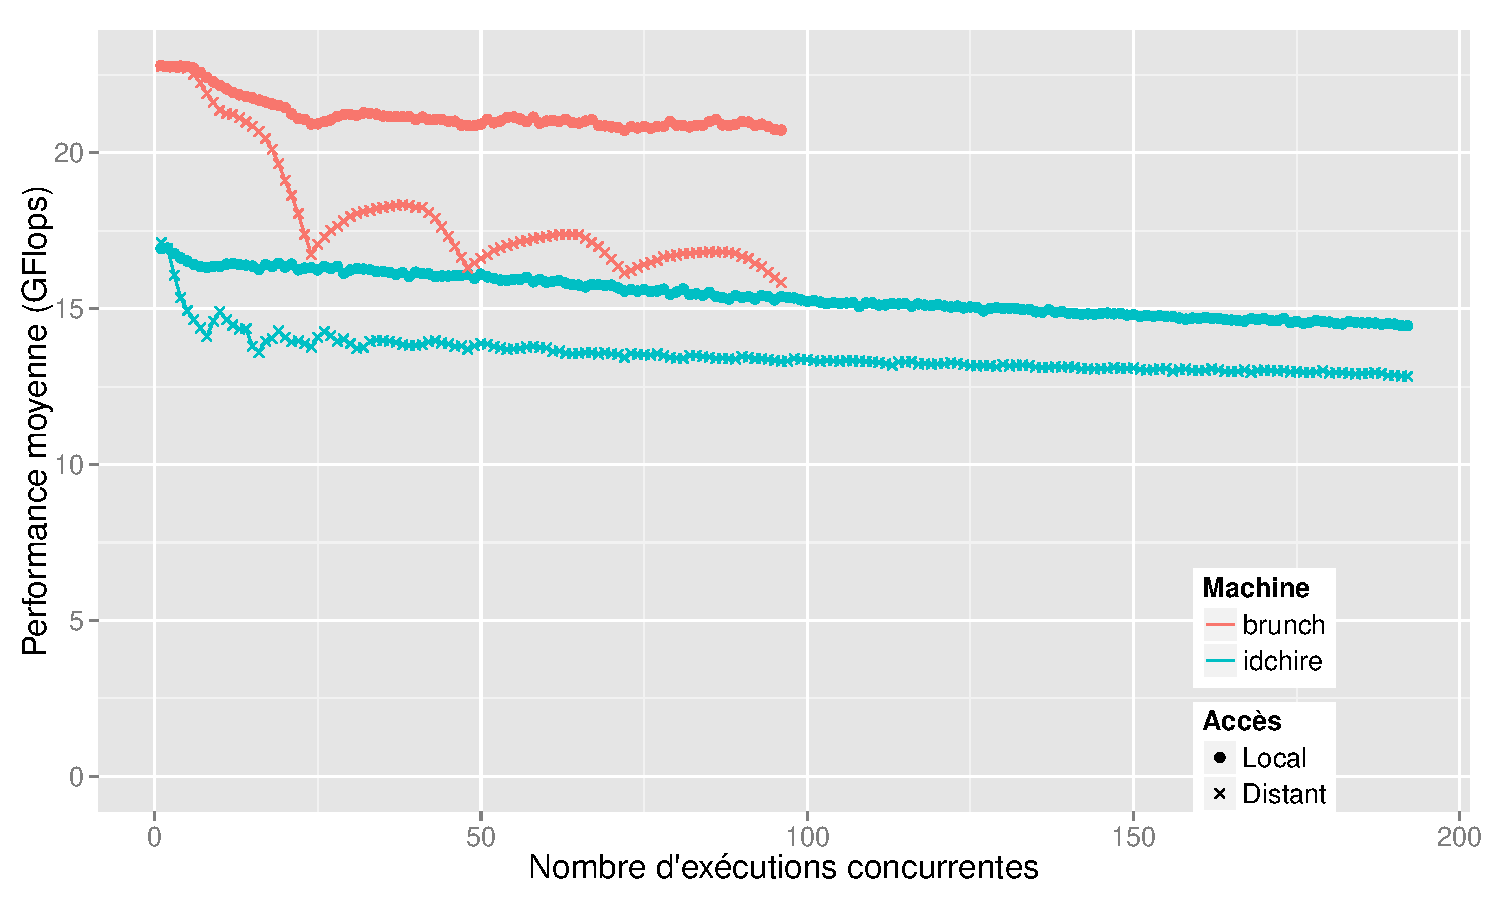
\includegraphics[width=0.95\textwidth]{graph/kernel_comp_locality_gemm_512.pdf}
\end{figure}


\end{frame}


\begin{frame}
  \frametitle{Bilan}
  \begin{block}{Caractérisation des noyaux de l'application}
    Triple effet sur les performances :
    \begin{itemize}
      \item Baisse linéaire des perfs. (Corrélée aux caches miss L3)
      \item Différence local vs distant.
      \item Différence d'impact de la localité en fonction du jeu de données (ne tient pas dans le L3 pour 512).
    \end{itemize}
  \end{block}

  \begin{block}{Utilisation de l'outil}
    \begin{itemize}
      \item Observations impossibles sans lui
      \item Flexible (caractérisation d'applications, du matériel)
    \end{itemize}
  \end{block}

  %\begin{block}{Motivation}
    %Régler le plus gros problème : la localité.
  %\end{block}

\end{frame}

\begin{frame}
\frametitle{Synthèse}


Données conséquentes sur les noyaux et leur comportement

\begin{itemize}
  \item possibilité de modéliser la performance attendue de l'application globale (simulation)
\end{itemize}

Identification de sources de variation de performances

\begin{itemize}
  \item Défauts de cache (liés aux Blas et au noyau)
  \item Placement des données : favoriser le rapprochement des tâches et des données dans le support exécutif
\end{itemize}

\end{frame}

\begin{frame}
  \frametitle{Méthodologie pour l'amélioration d'une application}
  \begin{minipage}[t]{0.36\linewidth}
    \begin{block}{Problématiques}
      \begin{itemize}
	{
	  \transparent{0.5}
	  \item Identifier les facteurs responsables
	  \item Chiffrer leur impact
	}
	\item Diminuer l'impact de ces facteurs
	{
	  \transparent{0.5}
	  \item Peut on prévoir les performances ?
	}
      \end{itemize}
    \end{block}
  \end{minipage}
      \hfill
  \begin{minipage}[t]{0.60\linewidth}
    \begin{figure}
      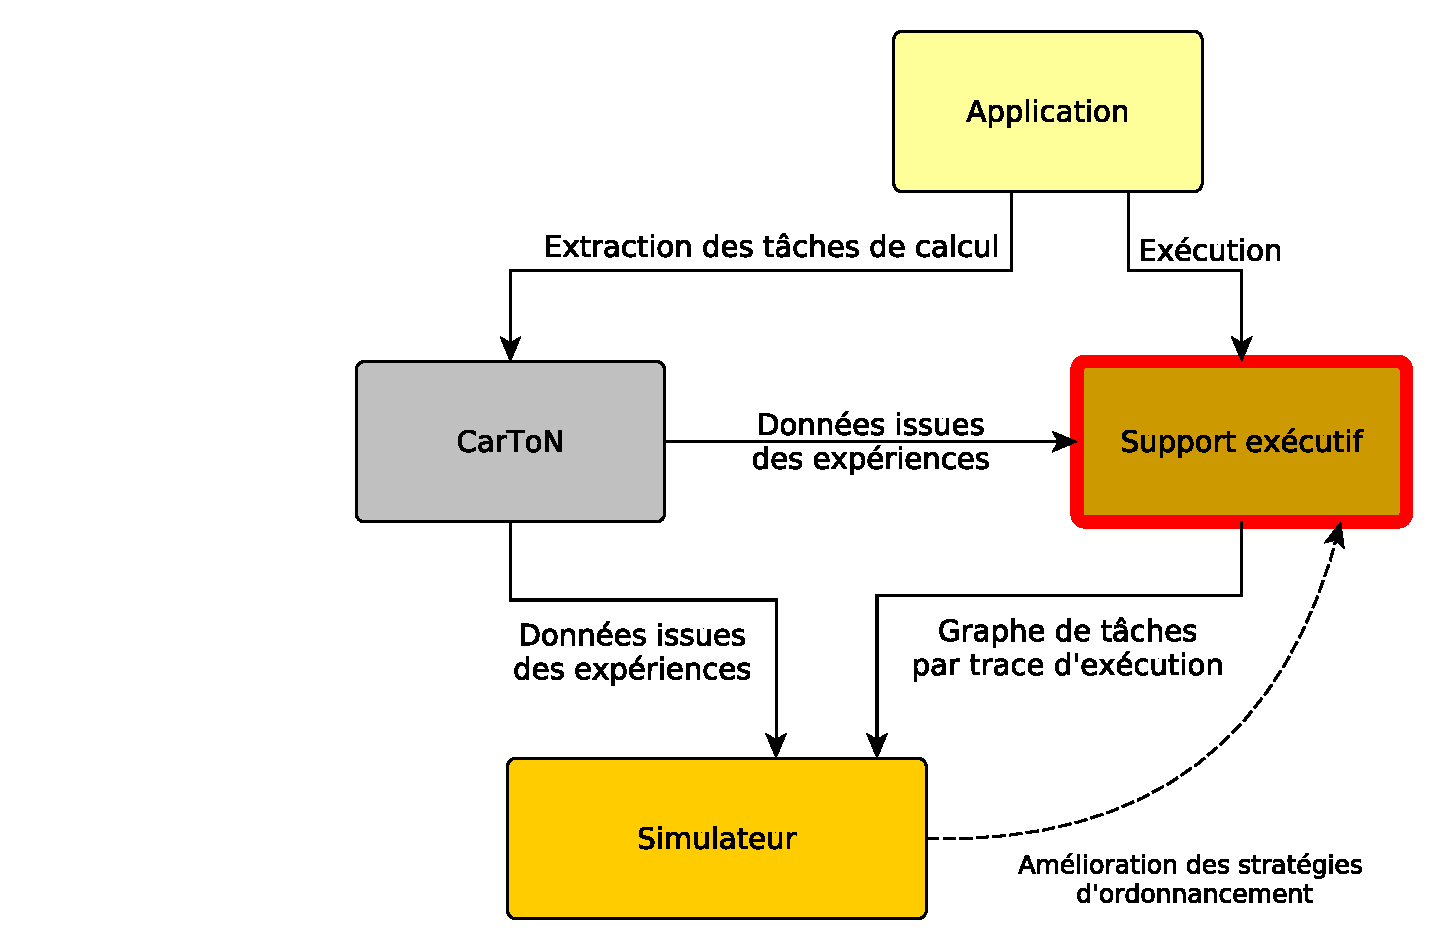
\includegraphics[width=\textwidth]{graph/big_picture-part2.pdf}%
    \end{figure}
  \end{minipage}
\end{frame}

\begin{frame}[fragile]
\frametitle{Rappel}

Application représentée sous forme de DAG

  \begin{minipage}[t]{0.46\linewidth}
  \begin{lstlisting}
#define N_BLOCS 3
for (int k = 0; k < N_BLOCS; k++) {
  #pragma omp task depend(inout:A(k,k))
  POTRF(A(k, k));

  for (int m = k+1; m < N_BLOCS; m++) {
    #pragma omp task depend(in:A(k,k))
                     depend(inout:A(m,k))
    TRSM(A(k, k), A(m, k));
  }

  for (int m = k+1; m < N_BLOCS; m++) {
    #pragma omp task depend(in:A(m,k))
                     depend(inout:A(k,k))
    SYRK(A(m, k), A(k, k));

    for (int n = k+1; n < m; n++) {
      #pragma omp task depend(in:A(m,k), A(n,k))
                       depend(inout:A(m,n))
      GEMM(A(n, k), A(m, k), A(m, n));
    }
  }
}
  \end{lstlisting}
  \end{minipage}
  \begin{minipage}[t]{0.46\linewidth}
    \vspace{-0.3cm}
    \begin{figure}
      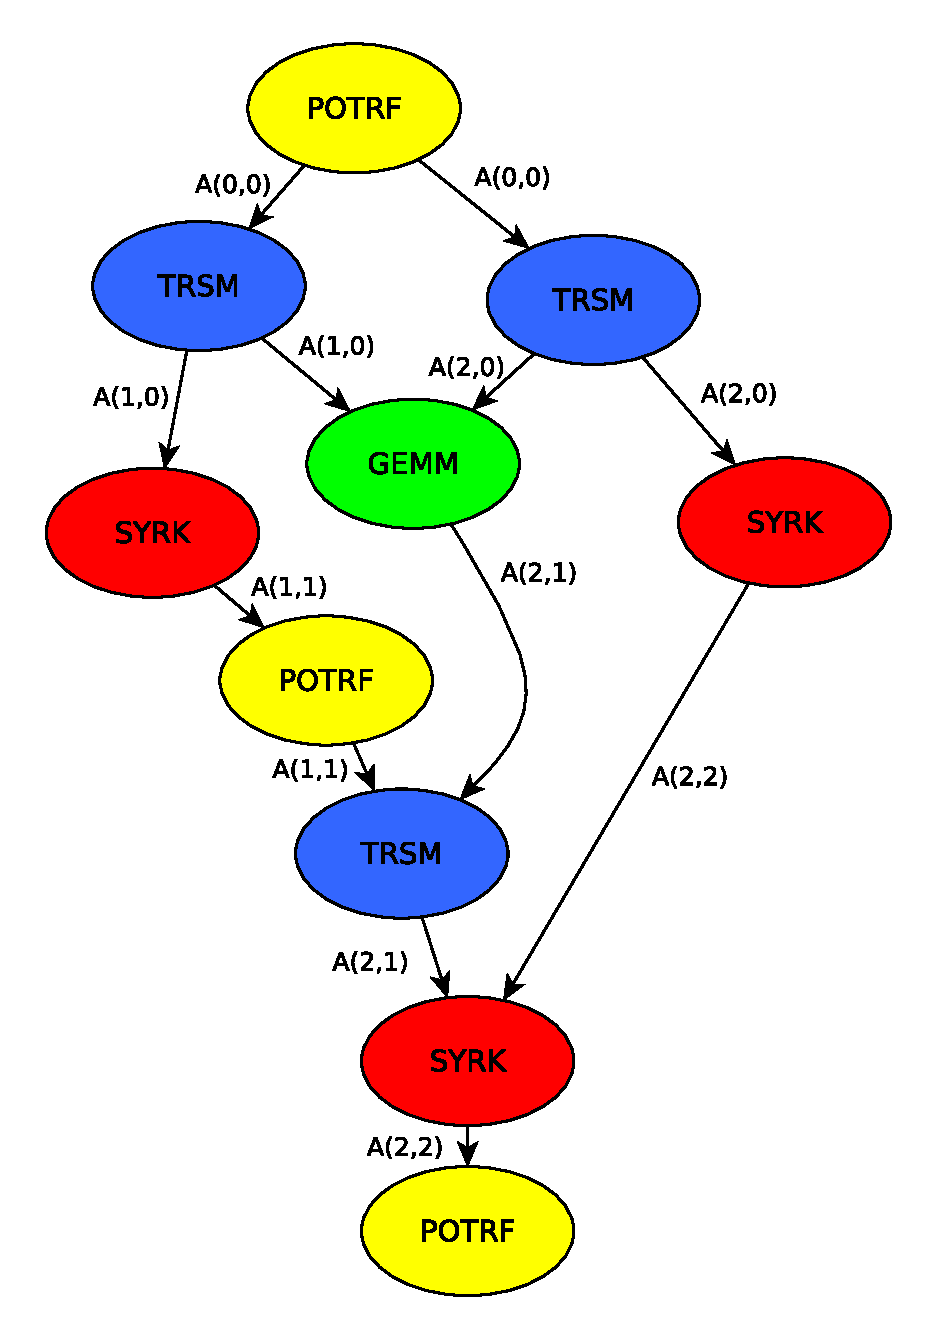
\includegraphics[width=0.9\textwidth]{graph/anim-dag/anim-8.pdf}%
    \end{figure}
  \end{minipage}
  %\begin{figure}
    %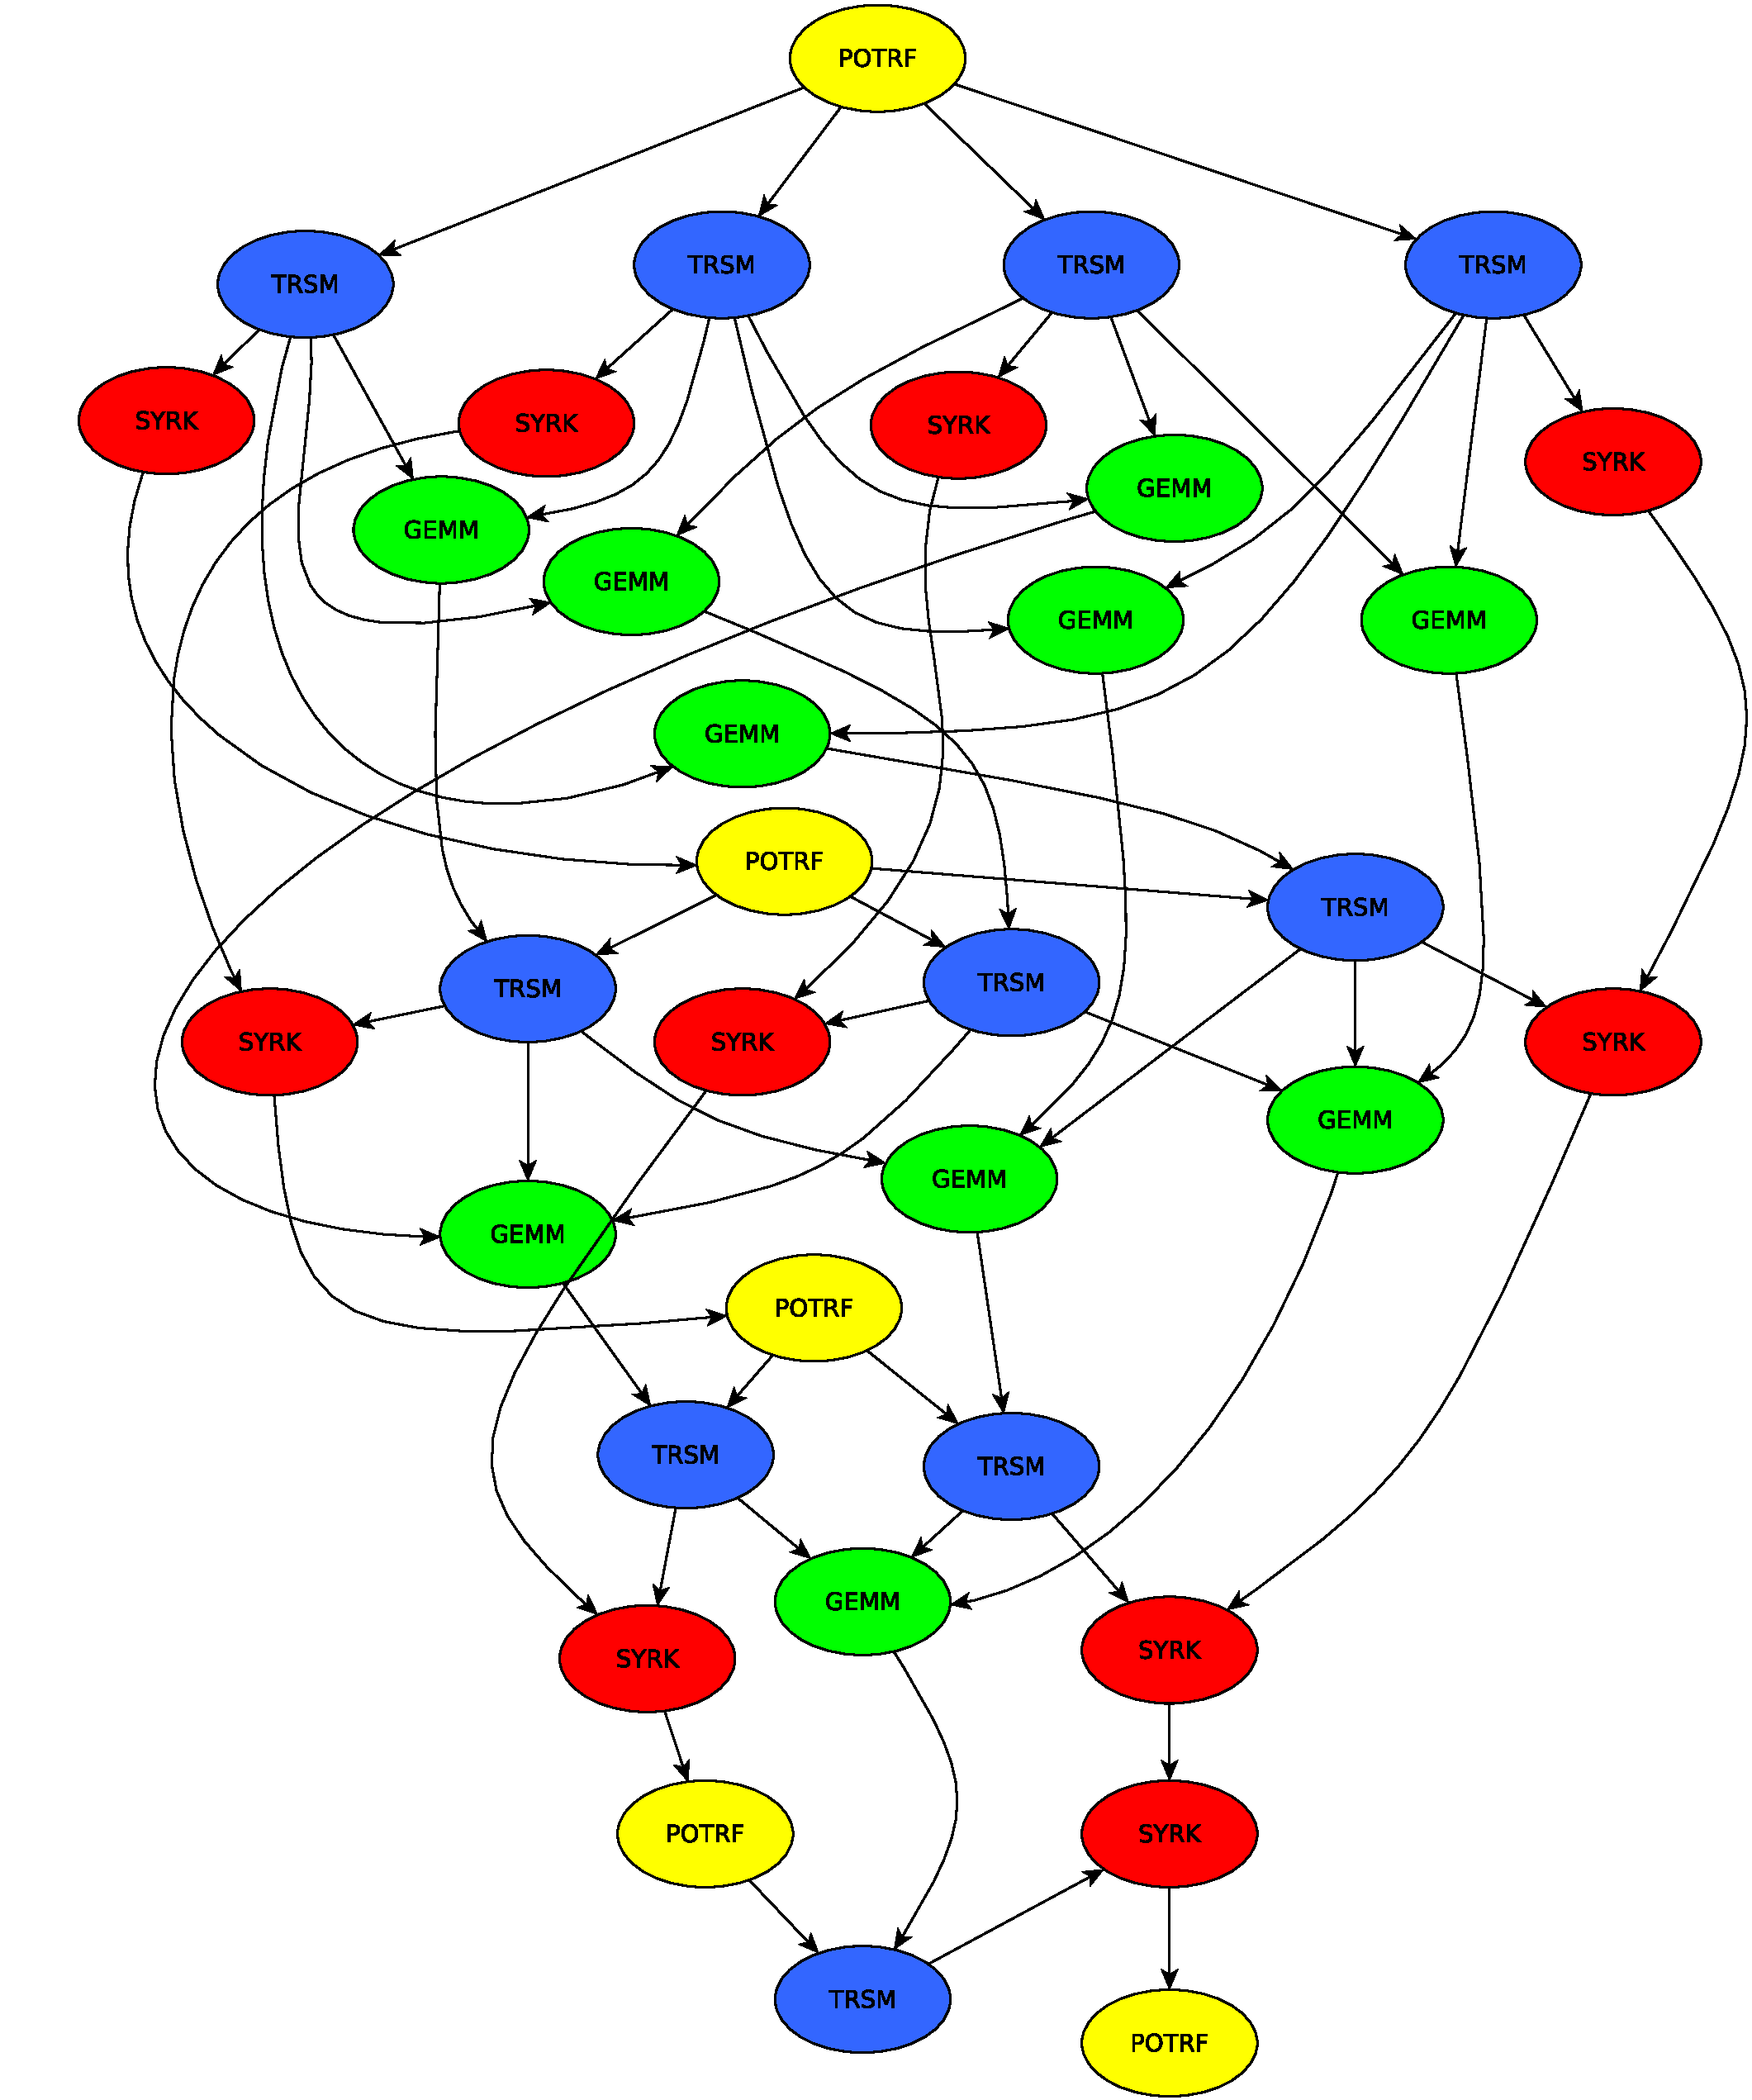
\includegraphics[width=0.4\textwidth]{graph/cholesky-dag-5.pdf}
  %\end{figure}

\end{frame}



\begin{frame}
  \frametitle{Travaux existants}
  \begin{exampleblock}{Objectif}
    Améliorer la localité des données au cours de l'exécution
  \end{exampleblock}
  \begin{block}{Groupement des calculs}
    Olivier et al., Clet-Ortega et al., Pilla et al.
    \begin{itemize}
      \item Partitionnement de la machine en "groupes"
      \item Équilibrage de charge favorisant les voisins dans le groupe
    \end{itemize}
  \end{block}

  \begin{block}{
    \only<1>{%
      Distribution des données, et placement des calculs%
    }%
    \only<2>{%
      \textbf{Distribution des données, et placement des calculs}%
    }%
  }
    HPF ;  StarPU, XKaapi (hétérogène) ; X10, Kaapi (distribué)
    %\begin{itemize}
      %\item HPF. Distribution de la \emph{possession} d'une donnée (OCR).
      %\item StarPU, XKaapi, ... -> Approche à la HEFT en hétérogène.
      %\item X10, Kaapi -> système distribué, prise en compte de la localité
    %\end{itemize}
  \end{block}

  \begin{block}{Migration dynamique des données, et conservation de la localité}
    OpenStream, ForestGOMP (support exécutif), Diener et al. (noyau)
    %\begin{itemize}
      %\item OpenStream. Placement des \emph{buffers} et des tâches.
      %\item ForestGOMP. Placement et migration de \emph{bulles}.
      %\item Diener et al. Observation (noyau) du comportement des threads, migration des pages et des threads.
    %\end{itemize}
  \end{block}

\end{frame}



\begin{frame}[fragile]
\frametitle{OpenMP : approches pour l'amélioration de la localité}

  \begin{block}{Dans le langage}
    Une dépendance $\neq$ utilisation d'une donnée
    \begin{itemize}
      \item Extension nécessaire pour le programmeur :

        \verb/affinity/ entre une tâche et ses données.
    \end{itemize}
  \end{block}

  \begin{block}{Dans le support exécutif}
    \begin{itemize}
      \item Vision hiérarchique de la machine
      \item Ordonnancement prenant en compte la localité des données (données fournies par le programmeur, informations dans les dépendances)
    \end{itemize}
    Modèle d'exécution : vol de travail.
  \end{block}

\end{frame}

\begin{frame}[fragile]
\frametitle{Influencer la localité des données : l'affinité}

\begin{block}{Clause affinité pour les \textit{tâches}}
  \begin{lstlisting}[language=c, numbers=none, basicstyle=\scriptsize]
#pragma omp task depend(in:A(k,k))
                 depend(inout:A(m,k))
                 affinity(data: A(m,k))
  TRSM(A(k, k), A(m, k));
  \end{lstlisting}
\end{block}


\begin{block}{Définition (discutée dans le standard)}
  \begin{lstlisting}[numbers=none, basicstyle=\scriptsize]
  affinity([node | thread | data]: expr[, strict])
  \end{lstlisting}
  Interprétation de \texttt{expr}~:
  \begin{itemize}
    \item \texttt{thread} -> indice d'un thread dans les \verb/OMP_PLACES/
    \item \texttt{node} -> indice d'un nœud NUMA (déduit des \verb/OMP_PLACES/)
    \item \texttt{data} -> adresse mémoire
  \end{itemize}
  \texttt{strict}~: la tâche \textbf{doit} s'exécuter sur la ressource.
\end{block}


\end{frame}


\begin{frame}[fragile]
\frametitle{Support exécutif : le vol de travail}

\begin{columns}[T,onlytextwidth]
  \column{0.60\textwidth}
  \vspace{1cm}

  \textbf{Vol de travail : deux étapes majeures}
  \begin{itemize}
    \item Workers \textit{poussent} une tâche dans une queue
    \item Voleurs \textit{sélectionnent} une queue où voler
  \end{itemize}
  \column{0.4\textwidth}
  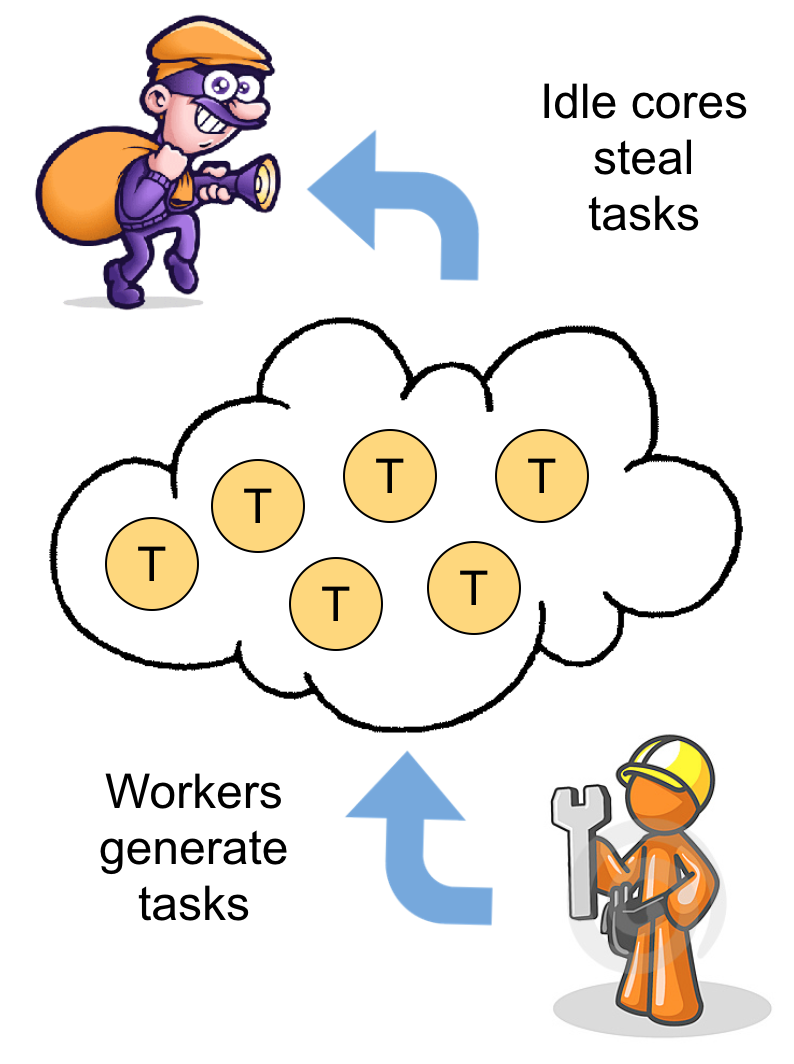
\includegraphics[scale=0.38]{graph/ws}
\end{columns}

\end{frame}

\begin{frame}
\frametitle{Support exécutif : maintient des tâches prêtes}

  Le support exécutif possède une file de tâches prêtes par élément de la hiérarchie.

\begin{figure}
  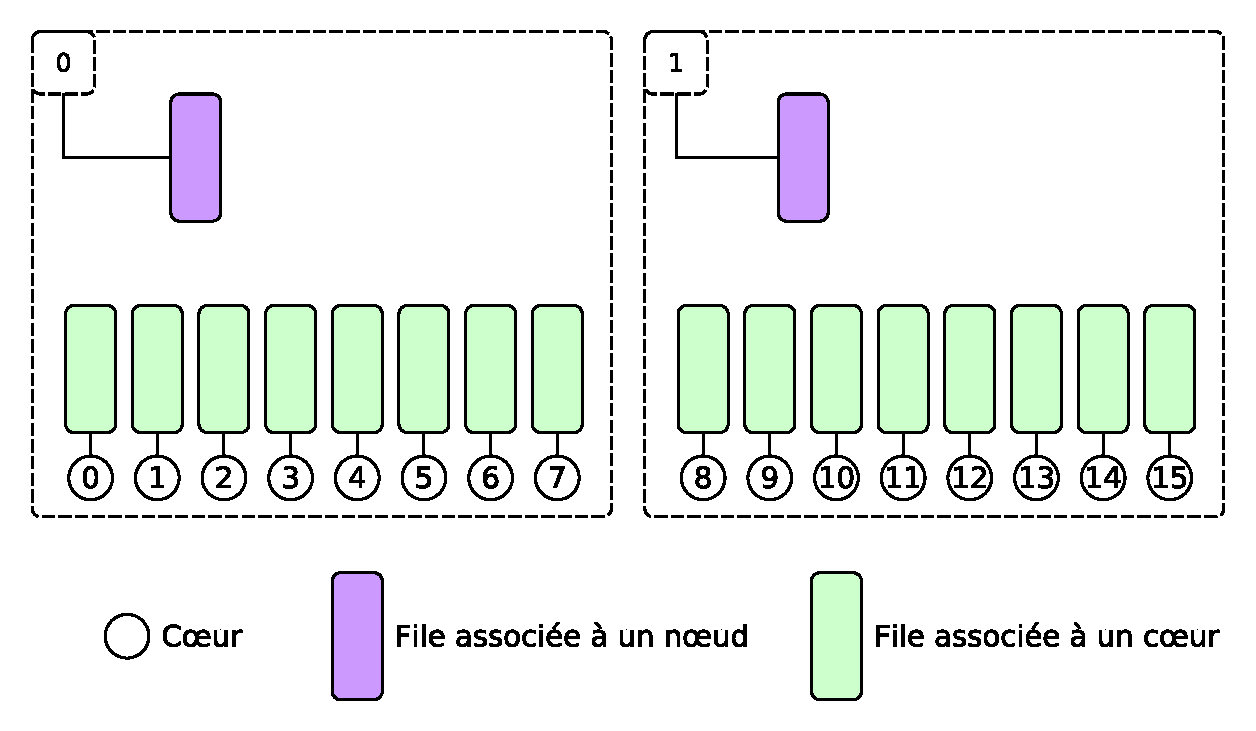
\includegraphics[width=0.8\textwidth]{graph/hierarchical_queues.pdf}
\end{figure}
\end{frame}

\begin{frame}
\frametitle{Exemple de stratégies d'ordonnancement}

\vspace{0.3cm}
Sélection d'une queue pour le placement d'une tâche prête
\begin{itemize}
  \item Si affinité : placement sur le nœud possédant la donnée, ou dans la queue du cœur si celui si est sur le nœud
  \item Sinon placement dans la queue du cœur locale
\end{itemize}
\vspace{0.5cm}

\uncover<2->{
Sélection d'une queue pour le vol
}
\begin{figure}
  \only<2> {%
    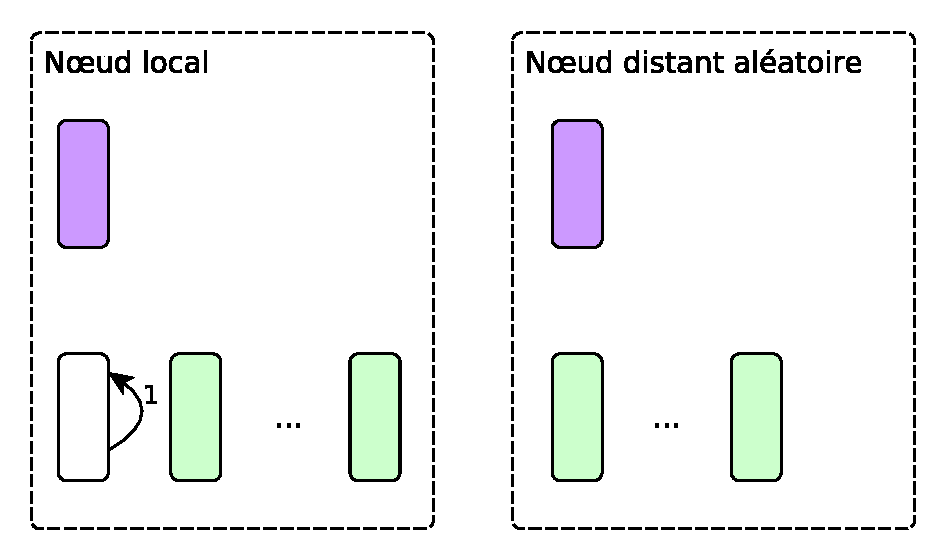
\includegraphics[width=0.6\textwidth]{graph/steal_strategies_anim_1.pdf}%
  }%
  \only<3> {%
    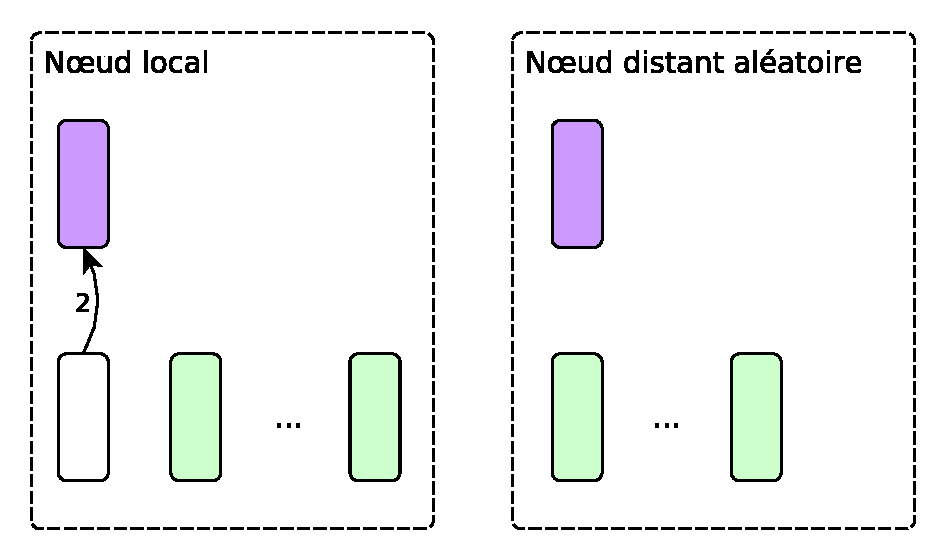
\includegraphics[width=0.6\textwidth]{graph/steal_strategies_anim_2.pdf}%
  }%
  \only<4> {%
    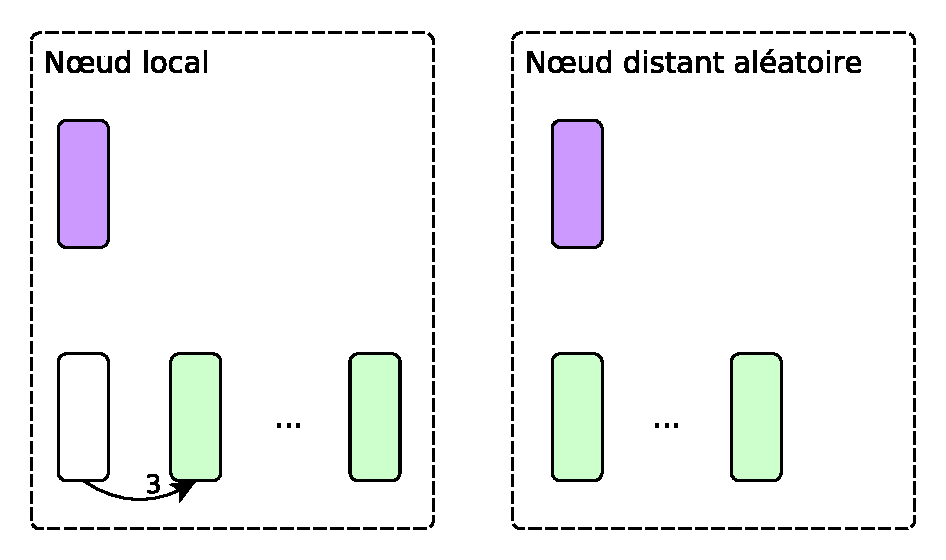
\includegraphics[width=0.6\textwidth]{graph/steal_strategies_anim_3.pdf}%
  }%
  \only<5> {%
    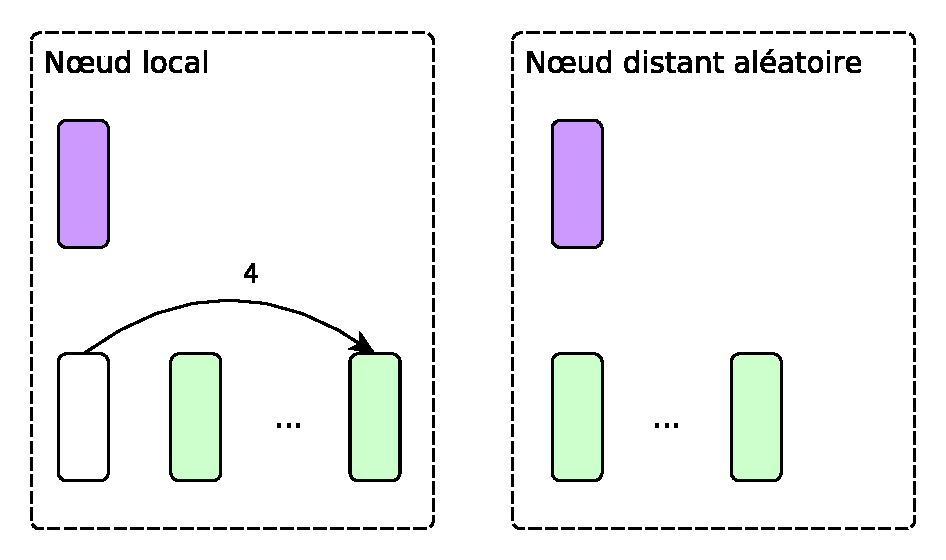
\includegraphics[width=0.6\textwidth]{graph/steal_strategies_anim_4.pdf}%
  }%
  \only<6> {%
    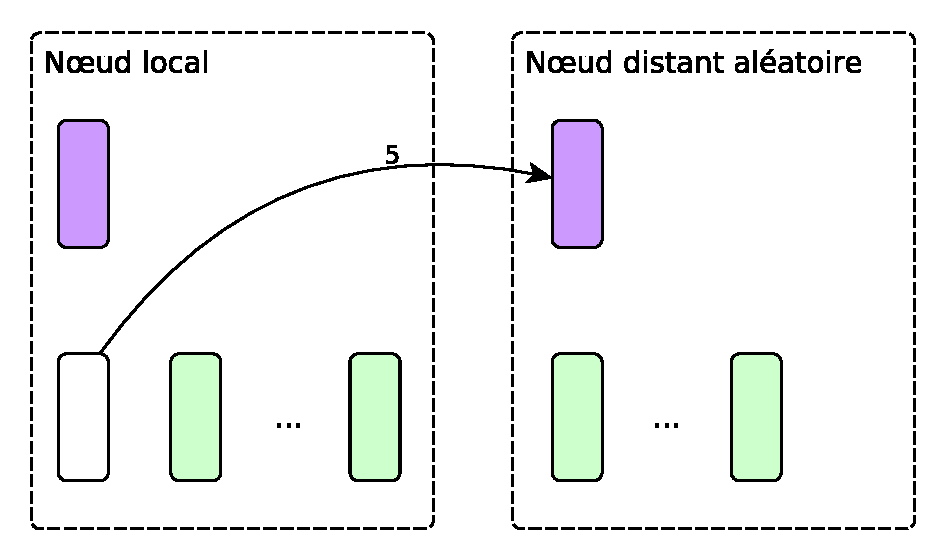
\includegraphics[width=0.6\textwidth]{graph/steal_strategies_anim_5.pdf}%
  }%
  \only<7> {%
    \includegraphics[width=0.6\textwidth]{graph/steal_strategies_anim_6.pdf}%
  }%
  \only<8> {%
    \includegraphics[width=0.6\textwidth]{graph/steal_strategies_anim_7.pdf}%
  }%
\end{figure}

\end{frame}

\begin{frame}
  \frametitle{Éléments de comparaison}

  \begin{block}{libGOMP}
    \begin{itemize}
      \item Livré avec GCC
      \item Pas de vision hiérarchique de la machine
      \item Queue centralisé, algorithme glouton
    \end{itemize}
  \end{block}

  \begin{block}{libOMP}
    \begin{itemize}
      \item Livré avec Clang (Intel)
      \item Pas de vision hiérarchique de la machine
      \item 1 queue par cœur, sélection aléatoire, placement local
    \end{itemize}
  \end{block}

  \begin{block}{libKOMP}
    \begin{itemize}
      \item libOMP étendue
      \item Queues hiérarchiques
      \item Vol hiérarchique, prise en compte de l'affinité
    \end{itemize}
  \end{block}

\end{frame}




\begin{frame}
  \frametitle{Comparaison des supports exécutif}
  Pic performance de Cholesky, en fonction de la taille de matrice, sur idchire
  \begin{figure}
    \includegraphics[width=0.8\textwidth]{graph/graph_details_cholesky_idchire.pdf}
  \end{figure}
  Meilleure taille de bloc pour chaque cas, distribution des blocs de données cyclique.
\end{frame}

\begin{frame}
  \frametitle{Comparaison des supports exécutif}
  Évaluation sur deux tailles choisies
  \includegraphics[width=0.9\textwidth]{graph/graph_all_cholesky_idchire.pdf}
\end{frame}

\begin{frame}
  \frametitle{Bilan de l'extension}

  \begin{block}{Impact sur les performances}
    Algèbre linéaire~:
    \begin{itemize}
      \item Différence significative (\textasciitilde 10\%) dès plusieurs nœuds NUMA
      \item Intuitions sur les situations favorables~:
      \begin{itemize}
	\item le parallélisme est présent
	\item le jeu de données sort du L3
      \end{itemize}
    \end{itemize}
  \end{block}

  \begin{block}{Quid des autres applications}
    Sur des applications itératives (Jacobi)~: performances des tâches comparables aux boucles.
  \end{block}
\end{frame}


\begin{frame}
  \frametitle{Méthodologie pour l'amélioration d'une application}
  \begin{minipage}[t]{0.36\linewidth}
    \begin{block}{Problématiques}
      \begin{itemize}
	{
	  \transparent{0.5}
	  \item Identifier les facteurs responsables
	  \item Chiffrer leur impact
	  \item Diminuer l'impact de ces facteurs
	}
	\item Peut on prévoir les performances ?
      \end{itemize}
    \end{block}
  \end{minipage}
      \hfill
  \begin{minipage}[t]{0.60\linewidth}
    \begin{figure}
      \includegraphics[width=\textwidth]{graph/big_picture-part3.pdf}%
    \end{figure}
  \end{minipage}
\end{frame}


\begin{frame}[fragile]
  \frametitle{Motivation pour la simulation}

  \begin{itemize}
    \item Développer dans un support exécutif réel à un coût.

      En simulation~:
      \begin{itemize}
	\item développement plus simple
	\item expérimentations plus rapides
      \end{itemize}

    \item Améliorer les décisions

      On a "le temps" pour les prendre

    \item Utilisation des caractéristiques des tâches

      Positionnement du support exécutif par rapport aux performances attendues.

    \item Simuler les programmes sur de nouvelles architectures

      Complexité~: modélisation
  \end{itemize}


\end{frame}

\begin{frame}[fragile]
  \frametitle{Composants du simulateur}
  \begin{itemize}
    \item Données

      Blocs de taille fixe, associés à un nœud (\emph{first-touch})

    \item Tâches

      Décomposées en plusieurs actions de trois types \verb/read/, \verb/write/, \verb/compute/

    \item Moteur exécutif

      Vol de travail
  \end{itemize}

\end{frame}

\begin{frame}[fragile]
  \frametitle{Modélisation}

  Modèle de coût global :

  \begin{itemize}
    \item Une tâche (\verb/read/+\verb/write/+\verb/compute/) = un coût unique
  \end{itemize}

  Coûts déterminés par les données de CarToN, en fonction du contexte d'exécution
  \begin{itemize}
    \item Accès local/distant
    \item Charge de la machine
  \end{itemize}

\end{frame}

\begin{frame}
  \frametitle{Stratégies et modèles considérés}

  \begin{block}{Vol de travail}
    Stratégies similaires à celles implémentées dans le support exécutif :
    \begin{itemize}
      \item Aléatoire
      \item Hiérarchique avec affinité.
    \end{itemize}
  \end{block}

  \begin{block}{Coûts des tâches}
    Objectif : borner l'exécution réelle.
    \begin{itemize}
      \item Maximum : meilleure performance observée via CarToN
      \item Distant : pire performance distante observée
      \item Deux niveaux + Affinité : utilisation du contexte d'exécution pour choisir le coût adapté
    \end{itemize}
  \end{block}

\end{frame}


\begin{frame}
  \frametitle{Évaluation}
  Matrice N=32768, BS=512 (~45000 tâches)
  \begin{figure}
    \includegraphics[width=\textwidth]{graph/simu_affinity_runtime_idchire.pdf}%
  \end{figure}


\end{frame}

\begin{frame}
  \frametitle{Évaluation}
  Matrice N=8192, BS=256 (~6000 tâches)
  \begin{figure}
    \only<1>{%
      \includegraphics[width=\textwidth]{graph/simu_affinity_8k_runtime_idchire.pdf}%
    }%
    \only<2>{%
      \includegraphics[width=\textwidth]{graph/simu_affinity_8k_runtime_idchire_ajuste.pdf}%
    }%
  \end{figure}


\end{frame}



\begin{frame}
  \frametitle{Bilan}

  \begin{block}{Bilan des premières expériences}
    \begin{itemize}
      \item Résultats assez réalistes vis à vis des tentatives existantes (Stanisic et al. dans SimGrid)
      \item Limite sur les cas à "faible" parallélisme
    \end{itemize}
  \end{block}
  \begin{block}{Perspectives}
    \begin{itemize}
      \item Utilisation de coûts plus précis
      \item Modélisation de la machine (caches, bande passante)
      \item Amélioration des distributions de données
    \end{itemize}
  \end{block}
\end{frame}

\begin{frame}
  \frametitle{Synthèse}

  \begin{minipage}[t]{0.36\linewidth}
    \begin{block}{Problématiques}
      \begin{itemize}
	\only<2->{
	  \item Caractérisation
	}
	\uncover<3->{
	  \item Amélioration
	}
	\uncover<4->{
	  \item Modélisation
	}
      \end{itemize}
    \end{block}
  \end{minipage}
      \hfill
  \begin{minipage}[t]{0.60\linewidth}
    \begin{figure}
      \only<1> {%
	\includegraphics[width=\textwidth]{graph/big_picture.pdf}%
      }%
      \only<2> {%
	\includegraphics[width=\textwidth]{graph/big_picture-synt-1.pdf}%
      }%
      \only<3> {%
	\includegraphics[width=\textwidth]{graph/big_picture-synt-2.pdf}%
      }%
      \only<4> {%
	\includegraphics[width=\textwidth]{graph/big_picture-synt-3.pdf}%
      }%
    \end{figure}
  \end{minipage}
  %\begin{block}{Processus complet pour une application}
    %\begin{itemize}
      %\item Observations générales et détaillées de l'application
      %\item Exécution prenant en compte les caractéristiques importantes
      %\item Ajustement des heuristiques d'ordonnancement via simulateur
    %\end{itemize}
  %\end{block}
\end{frame}


\begin{frame}
  \frametitle{Perspectives de la thèse}
  \begin{block}{CarToN}
    \begin{itemize}
      \item Se rapprocher des outils d'autotuning
      \item Étendre la définition des scénarios
    \end{itemize}
  \end{block}

  \begin{block}{Support exécutif}
    Meilleure collaboration compilateur/support exécutif
    \begin{itemize}
      \item informations supplémentaires (tailles des données)
    \end{itemize}
    Tâches à grain plus fin pour éviter la perte de scalabilité
    \begin{itemize}
      \item surcoût de création
      \item création parallèle
    \end{itemize}
  \end{block}

  \begin{block}{Simulation}
    \begin{itemize}
      \item Améliorer la modélisation (plus fine)
      \item Thèse Avalon/STORM, simulation de programmes OpenMP
    \end{itemize}
  \end{block}
\end{frame}

\begin{frame}
  \frametitle{Questions}

  Questions

\end{frame}

\begin{frame}
  \frametitle{Jacobi}

  TODO

\end{frame}

\begin{frame}
  \frametitle{backup1}

  miss L3

\end{frame}

\begin{frame}
  \frametitle{backup2}

  requete de vol/cœur

\end{frame}

\begin{frame}
  \frametitle{Cholesky avec barre d'erreur}

  \includegraphics[width=0.9\textwidth]{graph/graph_all_cholesky_idchire.pdf}

\end{frame}

\begin{frame}
\frametitle{TODO}

TODO : où placer ce slide ?

dgemm indépendant via l'outil, avec placement aléatoire de chacune des opérandes.
On constate qu'il y a deux bosses pour le cas 192, et que la bosse "min" est bien inférieure au minimum envisagé pour le cas précédent dans le simu.

Placement aléatoire de chacune des opérandes, taille 224.
(FIXME/NOTE : à comparer avec les distribs en situation réelle du slide 11, c'est le même cas !)

\begin{figure}
  \centering
  \includegraphics[width=0.8\textwidth]{graph/distrib_random_tool.pdf}
\end{figure}

\end{frame}



%\begin{frame}[fragile]
%\frametitle{Exemples d'applications par tâches}
%\begin{columns}[T,onlytextwidth]
  %\column{0.5\textwidth}
%\begin{onlyenv}<1>
  %\small{extrait d'un Jacobi (Stencil) :}
  %\begin{lstlisting}[numbers=none]
%for (int j = 0; j < ny; j += block_size) {
  %for (int i = 0; i < nx; i += block_size) {
    %/*... compute neighbors ...*/
%#pragma omp task
    %shared(/*...*/)
    %firstprivate(/*...*/) \
    %depend(out: unew[i][j]) \
    %depend(in: f[i][j], \
               %u[i][j], \
               %u[(i - xdm1)][j], \
               %u[i][(j + ydp1)], \
               %u[i][(j - ydm1)], \
               %u[(i + xdp1)][j])
    %compute_estimate(f, u, unew, /*...*/);
  %}
%}
%\end{lstlisting}

%\end{onlyenv}
  %\column{0.45\textwidth}
  %\small{extrait de Cholesky (Algèbre linéaire):}

%\begin{lstlisting}[numbers=none]
%/*...*/
%for (n = k+1; n < m; n++) {
%#pragma omp task depend(in:dA[k][n],
                           %dB[k][m])
                 %depend(inout:dC[n][m]])
    %cblas_dgemm(dA, dB, dC, /*...*/);
%}
%/*...*/
%\end{lstlisting}
%\end{columns}

%\uncover<2>{
%\begin{tikzpicture}[overlay, remember picture]
%\node[anchor=south west] (img2) at (1, -2) {\includegraphics[width=0.4\textwidth]{graph/dfg_depotrf.png}};
    %\end{tikzpicture}
%}
%\end{frame}



%\begin{frame}
%\frametitle{Motivations}

%\begin{figure}
  %\includegraphics[width=\textwidth]{./graph/jacobi_scale_iomp.pdf}
%\end{figure}

%\begin{alertblock}{Cause principale}
  %pas de localité temporelle dans la version avec tâches !
%\end{alertblock}
%\end{frame}



%\begin{frame}
%\frametitle{Applications et machines}

%\begin{block}{Suite de benchmarks KASTORS}
  %Applications utilisées :
  %\begin{itemize}
    %\item Algèbre linéaire (\textbf{Cholesky (dpotrf)}, QR, LU)
    %\item Stencil (Jacobi 2D)
  %\end{itemize}
%\end{block}

%\begin{block}{Machine : idchire}
    %\begin{itemize}
%\item Intel Xeon E5-4640 @ 2.4 GHz, Sandy Bridge
%\item 24 NUMA nodes, 8 cores per node, 192 total cores
    %\end{itemize}
%\end{block}

%\begin{block}{Logiciels}
  %Clang 3.9 + libKOMP (https://gitlab.inria.fr/openmp/libkomp/)
%\end{block}

%\end{frame}

%\begin{frame}
  %\frametitle{Étude de Cholesky}
  %\begin{center}
    %\includegraphics[width=\textwidth]{./graph/graph_evolution_cholesky.pdf}
  %\end{center}
%\end{frame}

%\begin{frame}
  %\frametitle{Prédiction}

  %\begin{block}{Quid de la prédiction ?}
    %Discussions avec Julien Langou (UC Denver) :
    %\begin{itemize}
      %\item Quelle(s) borne(s) sup théorique ?
      %\item Comment les améliorer ?
      %\item Distance des expériences vis à vis de la théorie ?
    %\end{itemize}
  %\end{block}
%\end{frame}

%\begin{frame}
  %\frametitle{Prédiction}
  %\begin{center}
    %\includegraphics[width=0.7\textwidth]{./graph/julien_upperbound_v1.pdf}
  %\end{center}
%\end{frame}

%\begin{frame}
  %\frametitle{Oops !}
  %\begin{alertblock}{Grosse divergence sur la courbe !}
    %\begin{itemize}
      %\item Le support exécutif est mauvais ?
      %\item Le modèle *théorique* mauvais ?
    %\end{itemize}
  %\end{alertblock}
%\end{frame}

%\begin{frame}
  %\frametitle{Observations}
  %\begin{block}{Observations}
    %\begin{itemize}
      %\item Pour un nombre de threads donné, temps des noyaux variables
      %\item Quelques "îlots" dans la distribution
    %\end{itemize}
  %\end{block}
%\end{frame}



%\begin{frame}
  %\frametitle{Évolution du temps des noyaux}
  %\begin{center}
    %\includegraphics[width=0.8\textwidth]{graph/cholesky_kernel_evolution.pdf}
  %\end{center}
%\end{frame}

%\begin{frame}
  %\frametitle{Prédiction}
  %% courbe bleue : critical path, revisité via perf max par cœur
  %% courbe rouge : upper bound, revisité via perf max par cœur
  %\begin{center}
    %\includegraphics[width=0.7\textwidth]{./graph/julien_upperbounds_v2.pdf}
  %\end{center}
%\end{frame}

%\begin{frame}
  %\frametitle{Vers une convergence}
  %\begin{block}{Première conclusion}
    %Le modèle théorique était trop optimiste
  %\end{block}
  %\begin{exampleblock}{Meilleure cohérence}
    %\begin{itemize}
      %\item Critical path mis à jour
      %\item Upper bound mis à jour
    %\end{itemize}
    %=> Baisse des limites théoriquement atteignables
  %\end{exampleblock}
  %\begin{block}{Aller plus loin}
    %\begin{itemize}
      %\item Il "manque" 250 Glops...
      %\item Comment identifier les facteurs de ces variations ?
    %\end{itemize}
  %\end{block}
%\end{frame}



%\begin{frame}[fragile]
%\frametitle{Faciliter les expériences à l'aide d'un outil}

    %Fournir un moyen simple et fiable pour les utilisateurs d'exécuter des noyaux, avec un contrôle précis sur le placement physique des données et sur l'exécution des noyaux.

  %\begin{block}{L'utilisateur fourni}
    %\begin{itemize}
      %\item Des noyaux et données.
      %\item Des scenario : quoi allouer, où et quand ; quoi lancer, où et quand.
      %\item Des indicateurs à observer (temps, compteurs de perf, ...)
    %\end{itemize}
  %\end{block}

  %\begin{block}{L'outil garanti}
    %\begin{itemize}
      %\item Une exécution fiable du scenario sur l'architecture cible.

      %\item Pas de surcoût = observation uniquement du comportement des noyaux.
    %\end{itemize}
  %\end{block}

%\end{frame}


%\begin{frame}[fragile]
%\frametitle{Fonctionnement}
%\noindent{%
%\begin{minipage}[t]{0.48\linewidth}
  %\begin{block}{"Support exécutif"}
    %\begin{itemize}
      %\item Un thread par cœur (pinned)
      %\item Noyaux empilés par cœur
      %\item Synchronisation si besoin
      %\item Relève des indicateurs avant/après
    %\end{itemize}
  %\end{block}
  %\begin{block}{Exemples}
    %\begin{itemize}
      %\uncover<2->{
        %\only<2>{
          %\item {\color{red}Données}
        %}
        %\only<3-4>{
          %\item Données
        %}
      %}
      %\uncover<3->{
	%\only<3>{
		%\item {\color{red}Actions}
	%}
	%\only<4>{
		%\item Actions
	%}
      %}
      %\uncover<4->{
        %\item {\color{red}Indicateurs}
      %}
    %\end{itemize}
  %\end{block}
%\end{minipage}}%
%\hfill%
%\begin{minipage}[t]{0.48\linewidth}

  %\begin{onlyenv}<2>
  %\begin{lstlisting}[numbers=none,language=yaml]
%scenario:
  %# ...
  %data:
    %- a:
      %- type: "double *"
    %- b:
      %- type: "double *"
    %- c:
      %- type: "double *"
    %- block_size:
      %- type: "int"
      %- value: 256
  %# ...
%\end{lstlisting}
  %\end{onlyenv}
  %\begin{onlyenv}<3>
  %\begin{lstlisting}[numbers=none,language=yaml]
%scenario:
  %# ...
  %actions:
    %- kernel: init_blas_bloc
      %sync: false
      %params:
      %- a
      %- block_size
      %core: 0
      %repeat: 1
    %- kernel: dgemm
      %sync: false
      %params:
      %- a
      %- b
      %- c
      %- block_size
      %core: 0
      %repeat: 50
%\end{lstlisting}
  %\end{onlyenv}
  %\begin{onlyenv}<4>
  %\begin{lstlisting}[numbers=none,language=yaml]
%scenario:
  %# ...
  %watchers:
    %flops_dgemm:
      %- block_size
    %papi:
      %- PAPI_TOT_CYC
      %- PAPI_L3_TCM
%\end{lstlisting}
  %\end{onlyenv}
%\end{minipage}

%\end{frame}
%\begin{frame}
  %\frametitle{Scenario simple d'oservation des dgemm}
  %\begin{block}{dgemm}
    %Multiplication de matrice : C = A*B + C
    %\begin{itemize}
      %\item Dominant dans Cholesky !
      %\item A et B : lu
      %\item C : lu et écrit
    %\end{itemize}
  %\end{block}

  %\begin{block}{Scenario}
    %\begin{itemize}
      %\item Matrices carrées (..., 256, 512, ...)
      %\item Allocation des données sur le nœud local, ou un nœud distant
      %\item Exécution simultanée de 50 dgemm indépendants sur N cœurs (1->192)
      %\item Observation des GFlops.
    %\end{itemize}
  %\end{block}


%\end{frame}

%\begin{frame}
  %\frametitle{Résultats synthétiques}
  %\begin{center}
    %\includegraphics[width=\textwidth]{./graph/dgemm_local_vs_remote.pdf}
  %\end{center}

%\end{frame}
%\begin{frame}[fragile]
%\frametitle{What information dœs it have?}


        %\begin{lstlisting}
%void foo(double *a, size\_t blocksize) {
  %#pragma omp parallel num_threads(3)
  %{
    %#pragma omp task depend(out:a[0:blocksize])
      %write_on(a);
    %#pragma omp task depend(in:a[0:blocksize])
      %display(a);
  %}
%}
        %\end{lstlisting}
%\noindent{%
%\begin{minipage}[t]{0.48\linewidth}
  %\begin{block}{Available:}
    %\begin{itemize}
      %\item DAG
      %\item Size of data manipulated
      %\item Operations done on the data
    %\end{itemize}
  %\end{block}
%\end{minipage}}%
%\hfill%
%\begin{minipage}[t]{0.48\linewidth}
  %\begin{block}{Deducible:}
    %\begin{itemize}
      %\item Data placement on the architecture
      %\item "Importance" of a task
    %\end{itemize}
  %\end{block}
%\end{minipage}


%\end{frame}



%\begin{frame}[fragile]
%\frametitle{Moyens actuels de contrôler l'affinité}

%\begin{block}{Affinité pour les threads}
  %\begin{itemize}
    %\item Définir des \verb/places/ (à travers \verb/OMP_PLACES/)
    %\item Utiliser \verb/proc_bind/ pour utiliser une politique de placement des threads spécifique
  %\end{itemize}
%\end{block}

%\begin{block}{Affinité entre une tâche et une donnée ?}
  %\begin{itemize}
    %\item Allocation mémoire \verb/first-touch/ (plupart des Linux)
    %\item Librairies spécifiques à l'allocation de données
  %\end{itemize}
  %Pas (encore) de support dans le standard
%\end{block}

%\end{frame}

%\begin{frame}[fragile]
%\frametitle{Approaches}

  %\begin{block}{Programmer's point of view}
    %\begin{itemize}
      %\item OpenMP compiler's extension

        %\verb/affinity/ between a task and its data (core/NUMA node level)
    %\end{itemize}
  %\end{block}

  %\begin{block}{Runtime's point of view}
    %\begin{itemize}
      %\item Hierarchical workstealing
      %\item Locality-aware schedulers (based on programmer hints, or dep information)
    %\end{itemize}
  %\end{block}

%\end{frame}


%\begin{frame}[fragile]
%\frametitle{Approches en discussion}

%\begin{block}{Clause affinité pour les tâches}
%Exprimer une affinité entre une tâche et "quelque chose" sur la machine
  %\begin{itemize}
    %\item Thread

      %\textcolor{YellowOrange}{
      %Cette tâche devrait être exécutée près de ce thread
    %}
    %\item Donnée

      %\textcolor{YellowOrange}{
      %Cette tâche devrait être exécutée proche de cette donnée
    %}
  %\end{itemize}

%\end{block}


%\end{frame}

%- méthodologie
	%- first touch
	%- affinity / ressource : core/numa
	%- affinity / data:
		%1/ partitionnement data => distribution des tâches d’initialisation
		%2/ clause affinity( data )

	%- s’appuie sur les extensions  (en profiter pour donner une sémantique assez précise)
		%- clause init
		%- clause affinity(core: cf ARB
		%- clause affinity( numa: cf ARB
		%- clause affinity( data:


%\begin{frame}[fragile]
%\frametitle{Additional extension}
%Needs to control the data distribution during initialization.

%We used an init clause for the parallel region:
%\begin{block}{Example}
  %\begin{lstlisting}[numbers=none]
  %#pragma omp parallel init(cyclicnuma)
  %#pragma omp single
  %{
    %for (/* all blocks */) {
      %#pragma omp task depend(out:block[0:])
      %init_block(block);
    %}
  %}
  %\end{lstlisting}
%\end{block}

%Distributing the task initializing the blocks will distribute the data (first-touch).

%In one of the upcoming talks, the ARB propose a concrete approache using affinity on taskgroup for this!

%\end{frame}



%\begin{frame}[fragile]
%\frametitle{LibKOMP}

%\begin{block}{Base : support exécutif d'Intel}
  %\begin{itemize}
    %\item Branche 4.5, rebase 5.0 prévue Janvier 2018
    %\item Compatibilité avec icc/clang/gcc
  %\end{itemize}
%\end{block}

%\begin{block}{Extensions et ajout}
  %\begin{itemize}
    %\item Tâches : Queues hiérarchiques, gestion de l'affinité, taskname
    %\item Gestion via appels au runtime ou extension de Clang
    %\item Monitoring : Via OMPT, génération de traces d'exécution pour gantt/R/etc
  %\end{itemize}
%\end{block}

%En ligne : https://gitlab.inria.fr/openmp/libkomp

%Wiki : https://gitlab.inria.fr/openmp/libkomp/wikis/home
%\end{frame}



%\begin{frame}
%\frametitle{Évaluation}

%\begin{block}{benchmarks KASTORS}
  %Benchmarks spécifiques pour OpenMP 4.0

  %Noyaux utilisés :
  %\begin{itemize}
    %\item Cholesky (dpotrf)
    %\item QR (dgeqrf)
    %\item LU (dgetrf)
    %\item Jacobi
  %\end{itemize}

  %Cholesky, QR, et LU sont tirés de Plasma, adaptés pour utiliser OpenMP (algorithmes par bloc, utilisent les tâches avec dépendances).

  %Jacobi est une application de type stencil.
%\end{block}

%\end{frame}

%\begin{frame}
%\frametitle{Logiciels}

%\begin{block}{Compilateur et support exécutif}
    %\begin{itemize}
%\item Clang 3.9 + affinity + taskname
    %\end{itemize}

    %\begin{itemize}
%\item LibKOMP : basé sur le support exécutif Intel
%\item Gestion des tâches étendue : queues hiérarchiques, gestion de l'affinité
%\item Ajout d'une génération de traces d'exécution
    %\end{itemize}
%\end{block}

%\begin{block}{Mesures énergétiques}
    %\begin{itemize}
      %\item Échantillonnage de compteurs RAPL
      %\item Corrélation début/fin expérience via R
    %\end{itemize}
%\end{block}

%\end{frame}






%\begin{frame}
  %\frametitle{Comportement des différentes version de Jacobi}
  %\begin{center}
    %\includegraphics[width=\textwidth]{graph/jacobi_scale_iomp_komp.pdf}
  %\end{center}
  %\uncover<2>{
    %\begin{exampleblock}{Conclusion}
      %c'est possible d'atteindre les performances du \texttt{for} avec des tâches !
    %\end{exampleblock}
  %}
%\end{frame}

%\begin{frame}
  %\frametitle{Evaluating the distributions}
  %\begin{center}
    %\includegraphics[width=\textwidth]{graph/graph_distrib.pdf}
  %\end{center}
%\end{frame}

%\begin{frame}
  %\frametitle{Évaluation des stratégies (avec cyclicnuma)}
  %\begin{center}
    %\includegraphics[width=\textwidth]{graph/graph_all_strat.pdf}
  %\end{center}
%\end{frame}

%\begin{frame}
  %\frametitle{Description des trucs évalués}
  %Lister les choses qu'on a pu observer (init, stratégies, etc..)
  %Voir le temps qu'il y a pour parler des différents points
%\end{frame}

%\begin{frame}
  %\frametitle{Cholesky et QR avec une affinité \texttt{data} (idchire)}
  %\footnotesize Matrice : N=32k, BS=512
  %\begin{center}
    %\includegraphics[width=\textwidth]{graph/graph_dpotrf.pdf}
  %\end{center}
%\end{frame}

%\begin{frame}
  %%ça c'est sur idkat : perf équivalente, énergie -- !
  %%737 -> 5602
  %%750 -> 5267
  %%hors RAM -> 340 GFLOPS
  %%6284 - 5866 -> 418
  %% soit environ 80 GFLOPS d'écart -> la DRAM !

  %\frametitle{Consommation de la DRAM sur Cholesky (idkat)}
  %\footnotesize Matrice : N=32k, BS=512
  %\begin{center}
    %\includegraphics[width=\textwidth]{graph/graph_energy_dram_dpotrf.pdf}
  %\end{center}
%\end{frame}

%\begin{frame}

  %\frametitle{Profil énergétique de LU (N=32k, BS=512)}
  %\begin{center}
    %\includegraphics[width=0.8\textwidth]{graph/Rplot.pdf}
  %\end{center}
%\end{frame}


%\begin{frame}[fragile]
  %\frametitle{Conclusion}
  %\begin{block}{Affinité et localité}
    %\begin{itemize}
      %\item Problème de performance identifié et résolu
      %\item Effet "bonus" sur l'énergie
    %\end{itemize}
  %\end{block}

  %\begin{center}
    %Peut on faire mieux ?
  %\end{center}
%\end{frame}

%\section{Simulation}








%\begin{frame}
%\frametitle{Trying the easy way}
%\only<1>{
    %\begin{figure}
        %\includegraphics[width=\textwidth]{graph/graph_defaultmkl.pdf}
    %\end{figure}
    %\vspace{-25pt}
    %\tiny OMP\_NUM\_THREADS=n ./kernel size
%}
%\only<2>{
    %\begin{figure}
        %\includegraphics[width=\textwidth]{graph/graph_defaultmkl_ref.pdf}
    %\end{figure}
    %\vspace{-25pt}
    %\tiny Pic perf in \textcolor{red}{red} !
%}



%\end{frame}
%\begin{frame}
%\frametitle{Common way of dealing with this...}
%\begin{block}{Thread placement}
    %\begin{itemize}
%\item All on same node : reuse cache, nice if compute bound
%\item All distributed accross the machine : average data access faster
%\item Important : no thread migration !
    %\end{itemize}
%\end{block}
%\uncover<2->{
%\begin{block}{Memory distribution}
    %\begin{itemize}
        %\item All memory on the same node : high contention (cf mkl)
        %\item Memory spread accross the node may reduce contention
        %\item Encourage placement of threads near "their" memory
    %\end{itemize}
%\end{block}
%}
%\uncover<3->{
%\begin{block}{Algorithms input}
    %\begin{itemize}
        %\item Choose appropriate size/blocksize for each problem
    %\end{itemize}
%\end{block}
%}
%\end{frame}

%\begin{frame}
%\frametitle{Explicit threads placement and memory distribution}
    %\begin{figure}
        %\includegraphics[width=\textwidth]{graph/graph_16k_mkl.pdf}
    %\end{figure}
    %\vspace{-15pt}
    %\tiny OMP\_NUM\_THREADS=n KMP\_AFFINITY="granularity=fine,explicit,proclist=[...]" numactl -i (...) ./kernel size
%\end{frame}

%\begin{frame}
%\frametitle{Conclusion}
%\begin{alertblock}{Don't}
    %\begin{itemize}
%\item Let the system decide threads placement
    %\end{itemize}
%\end{alertblock}

%\begin{exampleblock}{Do}
    %\begin{itemize}
%\item Pin your threads to avoid migration
%\item Try different threads placement
%\item Control data initialization and distribution
    %\end{itemize}
%\end{exampleblock}

%\end{frame}

%\begin{frame}
%\frametitle{What about task-based OpenMP ?}
    %\begin{figure}
        %\includegraphics[width=\textwidth]{graph/graph_16k_allruntimes.pdf}
    %\end{figure}
    %\vspace{-15pt}
    %\tiny Using OMP\_PLACES to pin threads
%\end{frame}

%\begin{frame}
%\frametitle{Chosing the right blocksize}
    %\begin{figure}
        %\includegraphics[width=\textwidth]{graph/graph_16k_512_allruntimes.pdf}
    %\end{figure}
%\end{frame}

%\begin{frame}
%\frametitle{Conclusion}
%\begin{exampleblock}{Do}
    %\begin{itemize}
        %\item Give the right amount of work to your runtime
    %\end{itemize}
%\end{exampleblock}
%\begin{block}{Note}
    %\begin{itemize}
        %\item Runtimes should be able to better exploit small blocksizes
    %\end{itemize}
%\end{block}

%\end{frame}

%\begin{frame}
%\frametitle{Even more obvious on 32K matrices !}
%\only<1>{
    %\begin{figure}
        %\includegraphics[width=\textwidth]{graph/graph_32k.pdf}
    %\end{figure}
%}
%\only<2>{
    %\begin{figure}
        %\includegraphics[width=\textwidth]{graph/graph_32k_512.pdf}
    %\end{figure}
%}
%\end{frame}

%\begin{frame}
%\frametitle{Conclusion}
%\begin{block}{Performances don't rely only on runtime}
    %\begin{itemize}
%\item Be aware of grain
%\item Tune your inputs
    %\end{itemize}
%\end{block}
%\begin{block}{Performances aren't *that* bad}
    %\begin{itemize}
%\item Decent scaling up to $\approx$100 cores
%\item Still a big gap to experimental pic perf (dgemm)
    %\end{itemize}
%\end{block}

%\end{frame}

%\subsection{Some more tuning !}
%\begin{frame}
%\frametitle{Tuning threads placement}
%\begin{block}{Threads placement}
    %\begin{figure}
        %\includegraphics[width=0.8\textwidth]{graph/thread_placement.pdf}
    %\end{figure}
%\end{block}
%\end{frame}


%\begin{frame}[fragile]
%\frametitle{Tuning data distribution}
%\begin{block}{Data initialization}
    %In kastors : initialized accross all the nodes
%\end{block}

%\begin{block}{Distribution at runtime}
    %Using \verb/numactl --interleave=all/
%\end{block}


%\end{frame}

%\begin{frame}
%\frametitle{The big picture...}
    %\begin{figure}
        %\includegraphics[width=\textwidth]{graph/graph_32k_compare_grid.pdf}
    %\end{figure}
%\end{frame}


%\begin{frame}
%\frametitle{Impact of memory distribution + threads placement}
    %\begin{figure}
        %\includegraphics[width=\textwidth]{graph/graph_32k_compare.pdf}
    %\end{figure}
%\end{frame}

%\begin{frame}
%\frametitle{Conclusion}
%\begin{block}{Memory distribution}
    %Actually worst : data is already distributed during initialization
%\end{block}
%\begin{block}{Threads placement}
    %\begin{itemize}
        %\item Not much difference for low and high number of threads
        %\item Nice gain from spreading the threads otherwise
    %\end{itemize}
%\end{block}
%\end{frame}

%\begin{frame}
    %\frametitle{Pic perf summary}
    %\begin{figure}
        %\includegraphics[width=\textwidth]{graph/graph_32k_picperf.pdf}
    %\end{figure}
%\end{frame}
%\begin{frame}
%\frametitle{Overall conclusion}
%\begin{block}{Tuning matters}
    %\begin{itemize}
        %\item Find the right threads placement
        %\item Adapt memory distribution
        %\item Adapt the grain of your application
    %\end{itemize}
%\end{block}
%\end{frame}


%\section{Solving the scalability issue}

%\begin{frame}
%\frametitle{Still some performances to gain}
%\begin{block}{Next step ?}
    %\begin{itemize}
    %\item Improve the algorithm -> cf litterature
        %\item Tune the program to a specific architecture -> not portable
        %\item Improve the runtime/programming model
    %\end{itemize}
%\end{block}
%\end{frame}

%\begin{frame}
%\frametitle{Still some performances to gain}
%\begin{block}{Improving the programming model}
    %\begin{itemize}
    %\item Better architecture aware directives/clauses
        %\item More tools
    %\end{itemize}
%\end{block}
%\begin{block}{Improving the runtime}
    %\begin{itemize}
        %\item Better mapping of data+threads (needs information)
        %\item NUMA aware algorithm (task queue, barrier, etc)
    %\end{itemize}
%\end{block}
%\begin{block}{Ask for compiler help}
    %\begin{itemize}
        %\item Can help automatically detect dependencies, data placement, etc)
    %\end{itemize}
%\end{block}
%\end{frame}

%\begin{frame}[fragile]
    %\frametitle{Conclusion - Current Kaapi state}
%\begin{onlyenv}<1>%
    %Affinity extension, via OpenMP API
    %\begin{lstlisting}
    %[...]
%omp_set_task_affinity( CYCLIC(m,n,6,4), 1 );
%#pragma omp task depend(out:dA[0:ldam*tempnn])
%CORE_dplgsy( bump, tempmm, tempnn, dA, ldam, A.m, m*A.mb, n*A.nb, seed );
    %[...]
%\end{lstlisting}
%Using Klang-omp :
    %\begin{lstlisting}
    %[...]
%#pragma omp task depend(out:dA[0:ldam*tempnn]) affinity( CYCLIC(m,n,6,4) )
%CORE_dplgsy( bump, tempmm, tempnn, dA, ldam, A.m, m*A.mb, n*A.nb, seed );
    %[...]
%\end{lstlisting}
%\end{onlyenv}
%\only<2>{
    %\begin{figure}
        %\includegraphics[width=\textwidth]{graph/graph_32k_512_kaapi.pdf}
    %\end{figure}
%}
%\footnotesize Reminder : target architecture has 24 (4*6) NUMA nodes.
%\end{frame}

%\begin{frame}
    %\frametitle{Fin}
    %\begin{center}
    %Fin
    %\end{center}
%\end{frame}


%\appendix

%\begin{frame}
%\frametitle{Other ongoing works}
%\begin{block}{Using OMPT}
    %\begin{itemize}
%\item IOMP + HPCToolkit
%\item OMPT can be used to gather information about where a thread fetch its data from.

%\item We want a per-task view
    %\end{itemize}

%\end{block}
%\end{frame}

%\begin{frame}
    %\frametitle{Another threads placement (round robin)}
    %\begin{figure}
        %\includegraphics[width=\textwidth]{graph/graph_32k_compare_spreadnode.pdf}
    %\end{figure}
%\end{frame}


\end{document}
